% =================================================================
% RESEARCH PAPER TEMPLATE / 研究论文模板
% =================================================================
% Single-column preprint layout -- journal-submission convention:
% manuscripts are prepared single column; two-column is applied by
% the publisher at final typesetting.
% =================================================================

% CHINESE PAPER SWITCH (中文论文开关) -- one line edit:
%   \documentclass line below -> \documentclass[fontset=none,10pt,a4paper]{ctexart}
% XeLaTeX is mandatory for both languages so the PDF contains the requested
% real fonts instead of pdfTeX-compatible substitutes.
\documentclass[fontset=none,10pt,a4paper]{ctexart}
\usepackage{iftex}
\ifXeTeX\else
  \PackageError{paper-template}{XeLaTeX is required}{Run xelatex; exact Times New Roman and Songti cannot be guaranteed under pdfLaTeX.}
\fi
\usepackage{fontspec}
% 优先使用模板规定的 Times New Roman 与宋体;构建机未安装时,退回度量兼容的
% Liberation Serif 与宋体风格的 Noto Serif CJK SC(交付说明中已注明)。
\IfFontExistsTF{Times New Roman}{
  \setmainfont{Times New Roman}
}{
  \setmainfont{Liberation Serif}
}
\makeatletter
\@ifclassloaded{ctexart}{
  \IfFontExistsTF{SimSun}{
    \setCJKmainfont{SimSun}
  }{
    \IfFontExistsTF{Songti SC}{
      \setCJKmainfont{Songti SC}
    }{
      \IfFontExistsTF{STSong}{
        \setCJKmainfont{STSong}
      }{
        \setCJKmainfont{Noto Serif CJK SC}
      }
    }
  }
  \IfFontExistsTF{SimHei}{
    \setCJKsansfont{SimHei}
  }{
    \IfFontExistsTF{Heiti SC}{\setCJKsansfont{Heiti SC}}{\setCJKsansfont{Noto Sans CJK SC}}
  }
}{}
\makeatother
\usepackage{graphicx}
\usepackage{amsmath,amssymb,amsfonts}
\usepackage[a4paper, margin=0.8in]{geometry}
\usepackage[numbers,sort&compress]{natbib}
\usepackage{booktabs}
\usepackage{microtype}
\usepackage{algorithm}
\usepackage{algpseudocode}
\usepackage{xcolor}
\usepackage{enumitem}
\usepackage{array}
\usepackage{tabularx}
\usepackage{multirow}
\usepackage{xurl}
\usepackage[hidelinks,unicode=true]{hyperref}
\urlstyle{same}
\usepackage{caption}
\usepackage{subcaption}
\usepackage{placeins}
\captionsetup{
  font=small,
  labelfont=normalfont,
  textfont=normalfont,
  labelsep=space,
  justification=justified,
  singlelinecheck=true,
  skip=6pt
}
\setlength{\textfloatsep}{12pt plus 2pt minus 2pt}
\setlength{\floatsep}{10pt plus 2pt minus 2pt}
\setlength{\intextsep}{10pt plus 2pt minus 2pt}
% Let figure-heavy manuscripts drain the float queue throughout the body.
% The final \FloatBarrier closes that queue; the following \clearpage makes
% the bibliography start on a clean page that contains no body text or floats.
\setcounter{topnumber}{5}
\setcounter{bottomnumber}{3}
\setcounter{totalnumber}{8}
\renewcommand{\topfraction}{0.90}
\renewcommand{\bottomfraction}{0.80}
\renewcommand{\textfraction}{0.07}
\renewcommand{\floatpagefraction}{0.70}
\setcounter{dbltopnumber}{4}
\renewcommand{\dbltopfraction}{0.90}
\renewcommand{\dblfloatpagefraction}{0.70}
\usepackage{fancyhdr}
\setlength{\headheight}{14pt}
\pagestyle{fancy}
\fancyhf{}
\fancyhead[L]{\small\nouppercase{\leftmark}}
\fancyhead[R]{\small\thepage}
\renewcommand{\headrulewidth}{0.4pt}
\fancypagestyle{plain}{
  \fancyhf{}
  \fancyfoot[C]{\small\thepage}
  \renewcommand{\headrulewidth}{0pt}
}
\renewcommand{\sectionmark}[1]{\markboth{\thesection\quad #1}{}}
% Chinese manuscripts use no running header by default. English manuscripts
% retain section-synchronised headers; the bibliography environment sets its
% own mark only when the reference heading begins.
\makeatletter
\@ifclassloaded{ctexart}{\pagestyle{plain}}{\pagestyle{fancy}}
\makeatother
% Diagrams: TikZ for flow/architecture, forest for hierarchies/trees (auto-spaced,
% no overlap). graphicx (above) provides \resizebox to clamp a figure to \linewidth.
\usepackage{tikz}
\usetikzlibrary{positioning, shapes.geometric, arrows.meta, fit, backgrounds, calc}
\usepackage{forest}

\newcommand{\todo}[1]{\textcolor{red}{[TODO: #1]}}

% 讲义用的定理类环境:标题用无衬线(黑体)常规字重,正文为常规字体。
\usepackage{amsthm}
\newtheoremstyle{handout}{0.6em}{0.6em}{\normalfont}{}{\sffamily}{}{0.8em}{}
\theoremstyle{handout}
\newtheorem{lemma}{引理}[section]
\newtheorem{proposition}{命题}
\newtheorem{definition}{定义}
\newtheorem{corollary}{推论}
\newtheorem{remark}{注}
\renewcommand{\proofname}{证明}
\newcolumntype{L}[1]{>{\raggedright\arraybackslash}p{#1}}
\setcounter{tocdepth}{2}

\title{\textbf{《疫情监测中的病例规模收益边界》理论详解与建议}}
% Production and review disclosures belong in the separate provenance report,
% not in the manuscript author block. Scientific status such as simulated
% evidence remains disclosed in the abstract, methods, and relevant captions.
\author{Apevon Science}
\date{2026 年 10 月}

\begin{document}
\maketitle
\normalfont\mdseries

\begin{abstract}
本讲义面向论文《疫情监测中的病例规模收益边界：估计目标、环境随机性与外部验证》的作者。讲义的目标是让作者能够不借助外部材料独立重现论文中的每一步推导，并说清每个数值的来源。讲义先列出前置知识、全部符号和模型假设，随后对命题 1 至命题 6、定义 1 与推论 1 逐一展开。每个结论都按同一顺序处理。先照录原式并注明原文式号，再写出每个参数的含义。然后逐步补全论文跳过的推导，并指明每一步所用的工具。最后用论文图 1 的参数给出数值例，并对应到论文的仿真与实证结果。

讲义的第二部分讨论从理论到实证的映射，涵盖可行广义最小二乘、经验交叉点、州聚类 Bootstrap、工具变量和稳健性检验，并汇总 199 条符号与数值核验的结果：187 条通过、10 条存在偏差、2 条不通过。代数结论全部成立。需要修改的内容集中在近似的方向、检验水平的措辞、离散功效的锯齿，以及截距和斜率与情景隐含值之间的口径差。讲义按原文行号列出这些问题和修改方案，并给出答辩问答与后续研究方向。附录给出负二项分布的 Poisson--Gamma 混合表示、二项抽稀的封闭性、全方差公式，以及 Fisher 信息与 Cram\'er--Rao 下界的完整证明。

\vspace{0.8em}
\noindent\textbf{关键词：}负二项分支过程；二项抽稀；全方差分解；方差交叉点；监测设计；推导核验
\end{abstract}


\clearpage
\tableofcontents
\clearpage

\setcounter{section}{-1}
\section{导读}\label{sec:guide}
\subsection{论文要回答的问题}

常规统计直觉认为样本越大推断越准。论文指出，个体超传播、不完全报告和共同环境扰动同时存在时，病例数与推断信息量之间的关系取决于估计目标。若目标是当期传播参数 $R_t$（论文称为目标 A），测量方差随期望报告规模 $m=\rho n$ 单调趋于零；若目标是跨期基础传播水平 $\bar R$（目标 B），单期估计留有一个不随规模下降的环境方差 $v_R$。论文据此把“病例规模在什么条件下不再主导推断误差”写成一个可计算的监测设计问题，核心量是规模项与环境项相等时的期望报告规模 $m_\times=A/v_R$。

\subsection{核心结论}

\begin{enumerate}
\item 命题 1 证明，给定上一代感染者数 $n$ 与当期 $R_t$，报告病例数 $C_t$ 严格服从负二项分布，$C_t/(\rho n)$ 是 $R_t$ 的最大似然估计，且在每个有限 $n$ 上精确达到 Cram\'er--Rao 下界，方差为 $R_t/(\rho n)+R_t^2/(kn)$，随规模单调趋于零。
\item 命题 2 用全方差公式把目标 B 的单期方差写成 $v_R+A/m$，其中 $A=\bar R+\rho(\bar R^2+v_R)/k$。环境项 $v_R$ 与规模无关，构成单期推断的方差下限。
\item 定义 1 给出交叉点 $m_\times=A/v_R$。在 $m=m_\times$ 处两项各占一半，规模翻倍带来的方差降幅为 $1/[2(1+m/m_\times)]$。以论文图 1 的参数（$\bar R=1.15$、$v_R=0.04$、$k=0.35$、$\rho=0.25$）计算，$A=2.1232$，$m_\times=53.08$，翻倍降幅在 $m=10$、$m_\times$、$200$ 处分别为 42.1\%、25.0\%、10.5\%。
\item 命题 3 比较两条扩大规模的路径：提高报告率 $\rho$ 只能消除漏报带来的抽样方差，扩大感染基数 $n$ 能让全部规模项同时衰减。
\item 命题 4 与推论 1 处理预算分配。在每期固定成本 $c_0$ 与单例成本 $c_1$ 下，最优单期规模为 $m^*=\sqrt{(c_0/c_1)m_\times}$，在 $c_0/c_1=10$ 与 $100$ 时分别为 23.0 与 72.9。环境扰动存在 AR(1) 相关时，有效期数近似 $T(1-r)/(1+r)$ 恒高估环境项，在 $T=26$、$r=0.8$ 时高估 20.5\%。
\item 命题 5 分解单步预测方差，命题 6 给出超临界增长的精确离散检验。离散检验的功效随 $n$ 呈锯齿状变化，在 $k=0.35$、$\delta=0.30$ 时功效首次达到 0.8 的样本量为 568，此后不再跌回 0.8 以下的稳定样本量为 581。
\item 实证部分使用全美 CDC NHSN 流感住院数据（16,218 个州周观测）。流行初期相对均方误差按 $a+b/D_t$ 递减，经验交叉点约 22.6 例/周，39\%--55\% 的误差份额落在与规模无关的截距上；达峰期常数均值偏移占总误差的 88.9\%。在 FluSight 集成预测和欧洲 11 国 COVID-19 数据中，规模项均为正，多模型集成把达峰期均值偏差占比压缩到 15.5\%。
\end{enumerate}

\subsection{逻辑链}

图~\ref{fig:logic} 给出全文的依赖关系。左列是两条模型假设，负二项分支传播与二项报告抽样共同给出命题 1 的单期精确分布。命题 1 在环境层取全方差得到命题 2，命题 2 的两项之比定义交叉点。交叉点再分别进入报告率与基数的比较（命题 3）、预算分配（命题 4 与推论 1）、预测分解（命题 5）和增长检验（命题 6）。右列是两类检验：命题 3 与命题 4 的规模关系由美国流感住院数据检验，命题 5 与命题 6 由更新过程仿真检验。虚线表示实证截距、斜率与理论参数之间的口径差，第~\ref{sec:empirical} 节与第~\ref{sec:checks} 节专门讨论这一反馈。

\begin{figure}[!tbp]
\centering
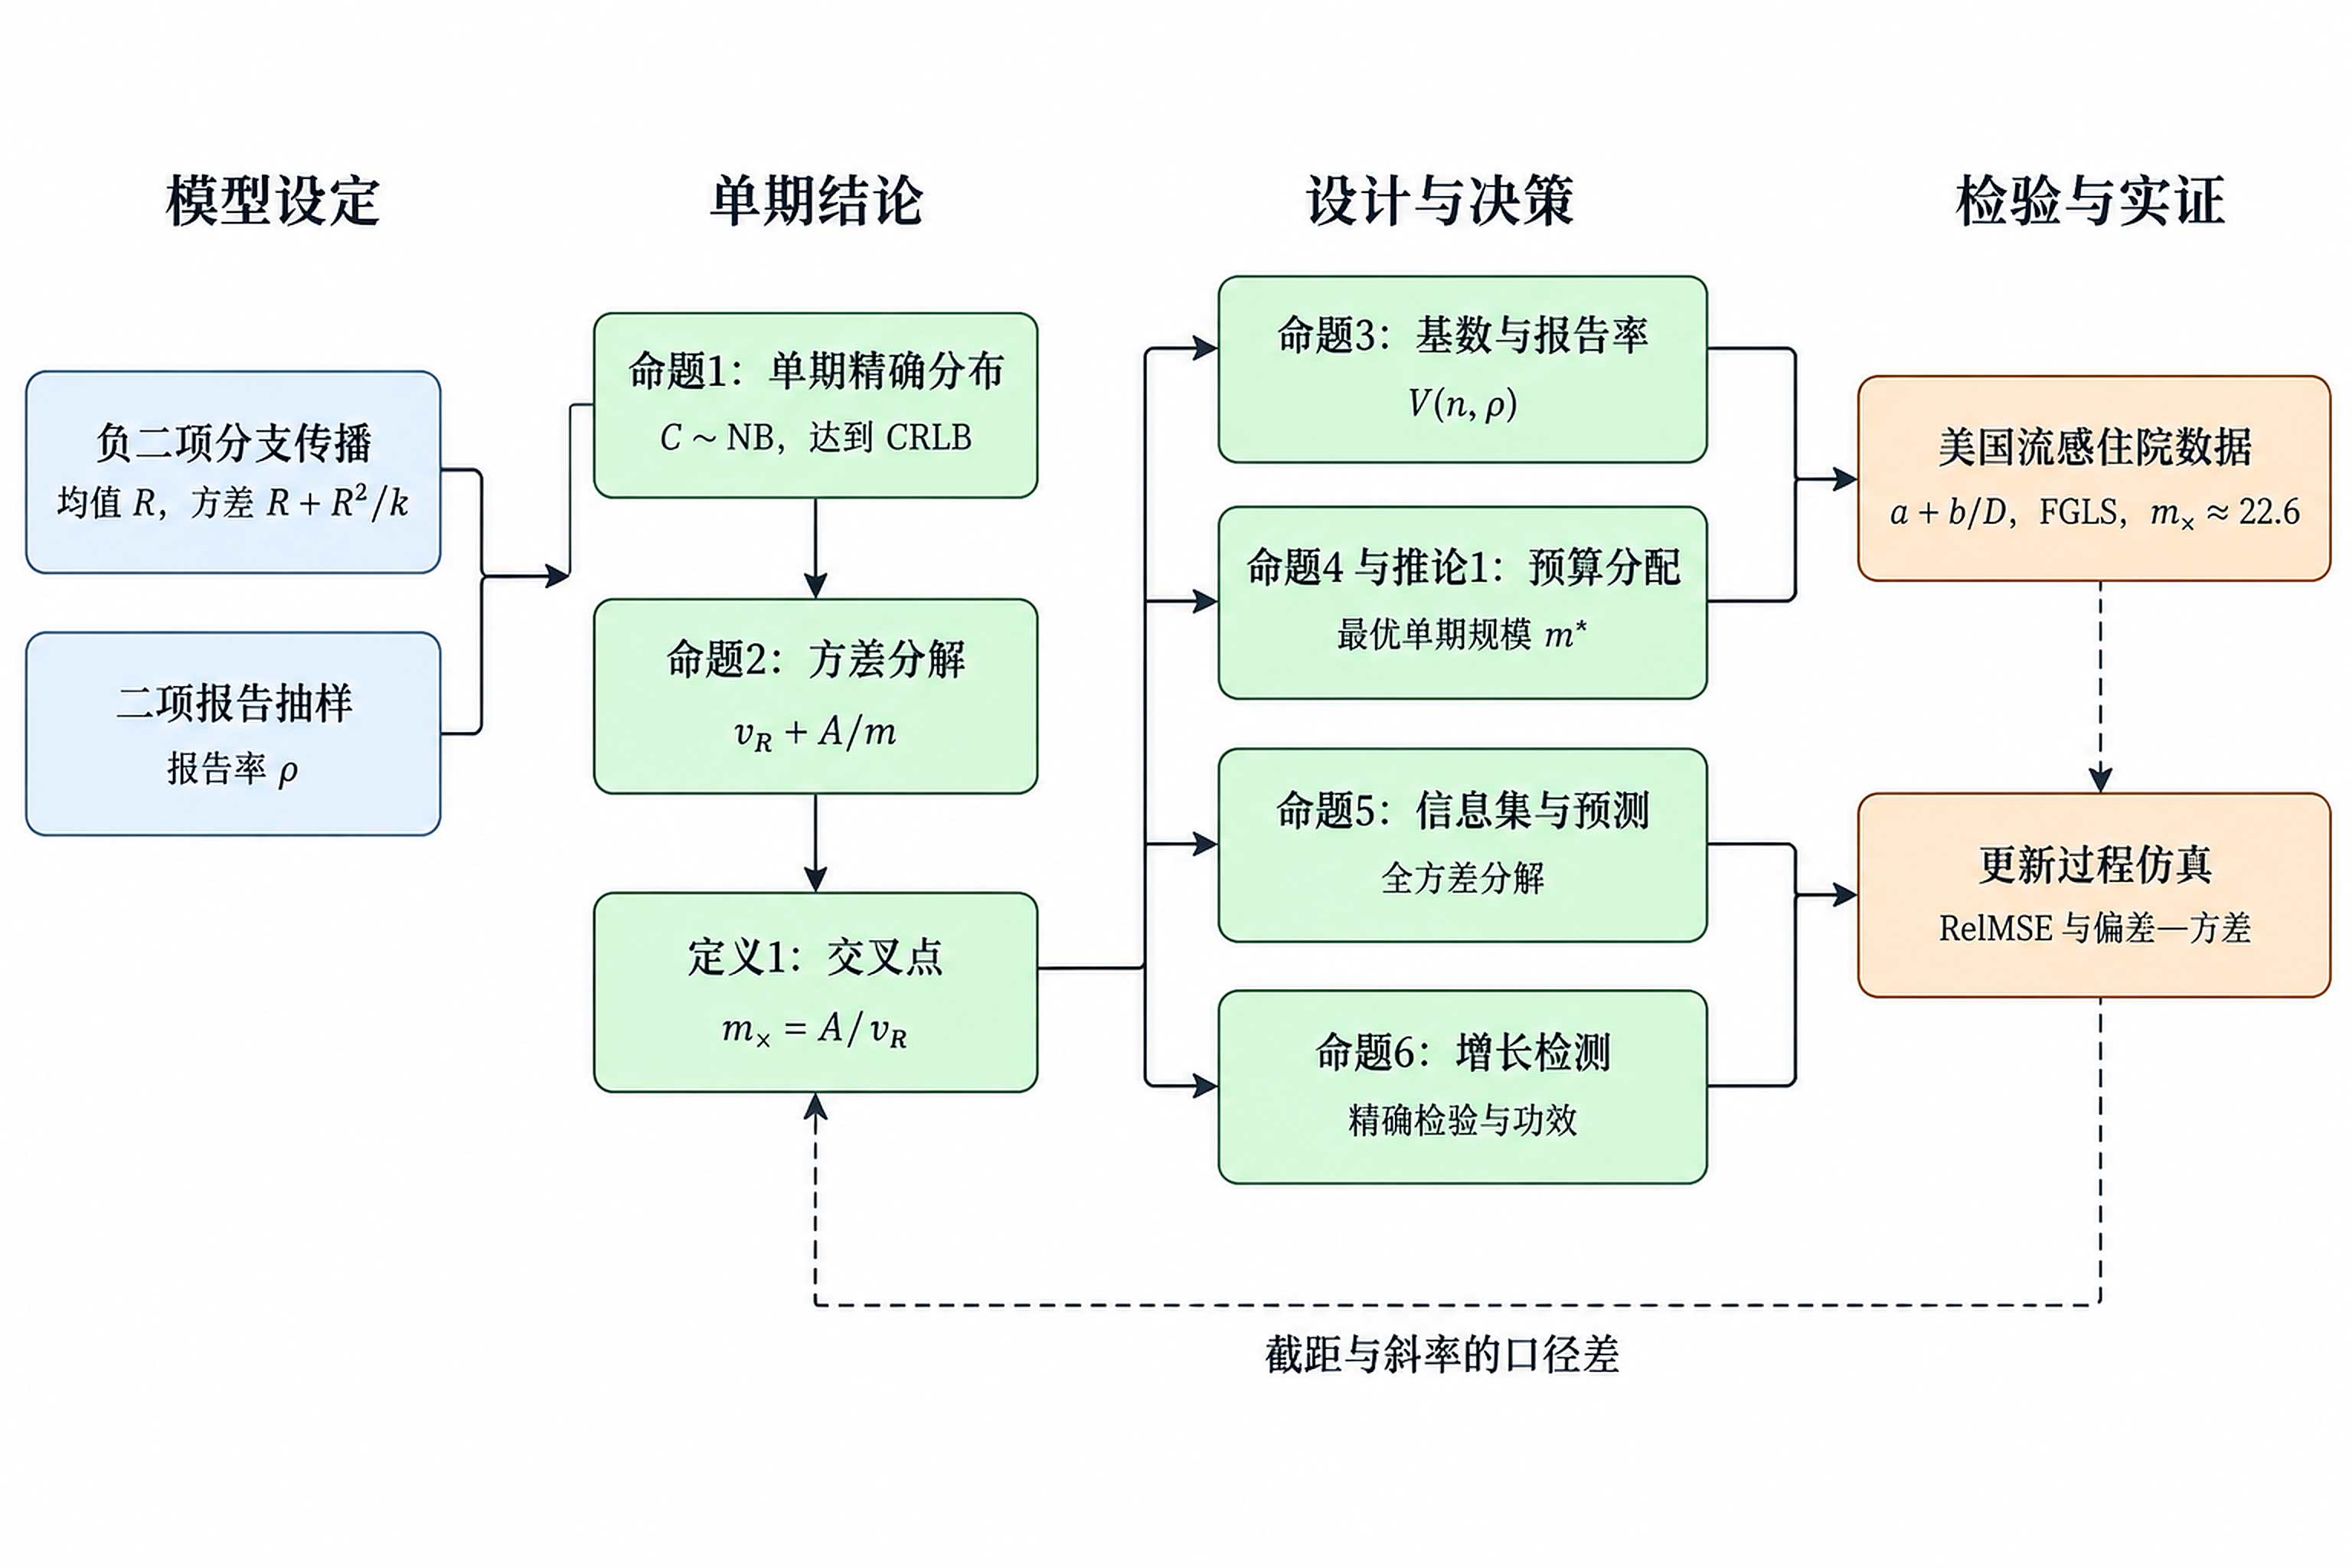
\includegraphics[width=0.95\linewidth]{figures/fig_logic_chain.png}
\caption{全文逻辑链。蓝色框是模型假设，绿色框是理论结论，橙色框是仿真与实证检验；实线箭头表示推导依赖，虚线表示实证截距与斜率和理论参数之间的口径差对交叉点定义的反馈。}
\label{fig:logic}
\end{figure}

\subsection{阅读建议}

第~\ref{sec:prereq} 节列出十项前置知识，前四项（负二项分布与概率生成函数、Fisher 信息与 Cram\'er--Rao 下界、全方差公式、AR(1) 有效样本量）是读懂第~\ref{sec:props} 节的必要条件。第~\ref{sec:symbols} 节与第~\ref{sec:model} 节可作为查阅表，推导中遇到陌生符号时回查。第~\ref{sec:props} 节建议按命题 1、命题 2、定义 1 的顺序在纸上逐步重推，这三步是答辩时最可能被要求现场推导的内容；命题 3 至命题 6 可在掌握前三步后按需阅读。第~\ref{sec:empirical} 节与第~\ref{sec:checks} 节对应答辩中关于实证口径的追问，第~\ref{sec:advice} 节给出修改方案与问答准备。附录~\ref{app:lemmas} 收录四个基础引理的完整证明，正文推导引用它们时不再重复。


\section{前置知识速查}\label{sec:prereq}
论文的推导只用到本科概率统计与计量经济学的标准工具，但这些工具在原文中都以一句话带过。表~\ref{tab:prereq} 按依赖顺序列出十项前置知识，前四项是读懂命题 1 至命题 4 的必要条件，第五至第八项按答辩追问的可能性排序，第九、十项服务于实证映射。每项给出一句话要点、在本讲义中的位置和一道自测题；能不看讲义完成自测题，即可认为该项已经掌握。

\begin{table}[!tbp]
\centering
\footnotesize
\caption{前置知识速查。位置一栏指本讲义的章节；自测题要求不看讲义独立完成。}
\label{tab:prereq}
\begin{tabular}{L{0.3cm}L{2.0cm}L{5.8cm}L{1.5cm}L{4.4cm}}
\toprule
序号 & 主题 & 一句话要点 & 位置 & 自测题 \\
\midrule
1 & 负二项分布与概率生成函数 & Poisson 的均值服从 Gamma 分布即得负二项分布；独立和的生成函数相乘，二项抽稀等价于把 $s$ 换成 $1-\rho+\rho s$，因此负二项抽稀后仍是负二项。 & 第~\ref{sec:model} 节、附录~\ref{app:lemmas} & 推出 $p^*=k/(k+\rho R)$ 与 $\operatorname{Var}(C)=\rho nR+\rho^2nR^2/k$。 \\
2 & Fisher 信息、CRLB 与完备性 & CRLB 取等当且仅当得分函数是估计量的仿射函数；指数族中充分统计量完备，其无偏函数即一致最小方差无偏估计。 & 命题 1 & 说明论文图 1(b) 中 0.988--1.017 的比值为何不能称为收敛。 \\
3 & 全方差公式 & $\operatorname{Var}(Y)=\operatorname{Var}(\mathbb{E}[Y\mid X])+\mathbb{E}[\operatorname{Var}(Y\mid X)]$；$\mathbb{E}[R^2]=\bar R^2+v_R$ 是最常被漏掉的一项。 & 命题 2、命题 5 & 推出 $v_R+A/m$ 与命题 5 的 $\mathrm{CV}^2$ 展开。 \\
4 & AR(1) 与有效样本量 & 相关样本均值的方差等于全部协方差之和除以 $T^2$；$T_{\rm eff}\approx T(1-r)/(1+r)$ 恒高估方差，相对误差约 $2r/[T(1-r^2)]$。 & 命题 4 & 用行和计数推出原文第 751 行的闭式，并计算 $T=26$、$r=0.8$ 时的误差。 \\
5 & Cochran 两阶段抽样 & 方差 $S_b^2/n+S_w^2/(nm)$ 与成本 $c_1'n+c_2'nm$ 给出 $m_{\rm opt}=\sqrt{(c_1'/c_2')(S_w^2/S_b^2)}$；推论 1 是它的换名形式。 & 推论 1 & 写出两者的符号对应，并说明小预算为何要整数枚举。 \\
6 & MLR 与 Karlin--Rubin 定理 & 似然比关于统计量单调时，单侧检验的水平在边界处取上确界，随机化单侧检验是一致最优势检验；非随机化离散检验的水平不超过 $\alpha$，功效呈锯齿状。 & 命题 6 & 说明“严格低于 $\alpha$”为何应改为“不超过 $\alpha$”，以及为何要报告稳定样本量。 \\
7 & 加权最小二乘与 FGLS & 均值设定正确时，任何只依赖回归元的权重都给出一致估计；最优权重是条件方差的倒数，权重只影响效率。 & 第~\ref{sec:empirical} 节 & 说明加权残差的 $\mathrm{CV}^2$ 从 5.32 降到 0.99 为何不足以支持 $1/\hat\mu^2$ 权重。 \\
8 & 聚类 Bootstrap & 以簇为单位重抽样，允许簇内任意相关，要求簇间独立且簇数足够；两维相关并存时用两向聚类。 & 第~\ref{sec:empirical} 节 & 说明按州聚类与按周聚类各自处理哪一种相关。 \\
9 & 工具变量与测量误差 & 回归元的经典测量误差使 OLS 斜率向零衰减，工具变量可以纠正；工具变量需要相关性（看第一阶段 $F$）与排除限制（不可检验）。 & 第~\ref{sec:empirical} 节 & 说明为何 $b_{\rm iv}>b_{\rm ols}$，以及工具变量为何不能消除分母噪声对 $b$ 的放大。 \\
10 & delta 法与比值估计 & $g(\hat\theta)$ 的方差近似为 $g'(\theta)^2\operatorname{Var}(\hat\theta)$；比值 $C/D$ 中分母的噪声以 $\mathbb{E}[G^2]\operatorname{Var}(\eta)$ 的形式进入方差。 & 第~\ref{sec:empirical} 节 & 推出 $b\approx[A+(1-\rho)(\bar R^2+v_R)\sum w^2]/\bar R^2$。 \\
\bottomrule
\end{tabular}
\end{table}

\subsection{推荐读物}

以下读物按表~\ref{tab:prereq} 的序号排列，每项只列最直接的一处。

\begin{enumerate}
\item 负二项分布与超传播参数 $k$ 的流行病学含义见 \citet{lloydsmith2005superspreading}；Poisson--Gamma 混合与概率生成函数见 \citet{casella2002statistical} 第 4 章。
\item Cram\'er--Rao 下界与 Lehmann--Scheff\'e 定理见 \citet{casella2002statistical} 第 7.3 节与 \citet{lehmann1998point} 第 2 章。
\item 条件期望与全方差公式见 \citet{casella2002statistical} 第 4.4 节。
\item AR(1) 自协方差与长程方差见 \citet{hamilton1994time} 第 3 章。
\item 两阶段抽样的最优分配见 \citet{cochran1977sampling} 第 10 章。
\item 单调似然比、Karlin--Rubin 定理与随机化检验见 \citet{lehmann2005testing} 第 3 章与 \citet{karlin1956theory}。
\item 加权最小二乘与可行广义最小二乘见 \citet{wooldridge2010econometric}。
\item 聚类 Bootstrap 与两向聚类见 \citet{cameron2008bootstrap,cameron2011robust}，实务要点见 \citet{cameron2015practitioner}。
\item 测量误差与工具变量见 \citet{wooldridge2010econometric} 第 4、5 章。
\item delta 法见 \citet{casella2002statistical} 第 5.5.4 节。
\end{enumerate}

\subsection{答辩前的最小准备}

答辩前至少应能在白板上用五分钟推完一条主线：负二项抽稀，命题 1 的 Fisher 信息，命题 2 的 $v_R+A/m$，交叉点 $m_\times$ 与翻倍降幅公式。第~\ref{sec:advice} 节列出的问答中，关于估计目标、$v_R$ 的可识别性、截距斜率口径和离散检验水平的四条最可能被追问，每条都应能用一句话作答。

表~\ref{tab:keynums} 列出需要记住的关键数值，它们在后文各节反复出现。

\begin{table}[!tbp]
\centering
\small
\caption{需要记住的关键数值及其出处。理论值按论文图 1 的参数计算，实证值取自论文第 5 节。}
\label{tab:keynums}
\begin{tabular}{L{5.2cm}L{3.6cm}L{6.4cm}}
\toprule
量 & 数值 & 出处与说明 \\
\midrule
规模相关方差系数 $A$ & 2.1232 & $\bar R=1.15$、$v_R=0.04$、$k=0.35$、$\rho=0.25$ \\
理论交叉点 $m_\times$ & 53.08 例/期 & $A/v_R$ \\
实证截距 $a$ 与斜率 $b$ & 0.0991 与 2.2434 & 流行初期 FGLS 拟合 \\
经验交叉点 $b/a$ & 22.6 例/周 & 区间 [13.7, 33.7] \\
情景隐含截距 & 0.014--0.029 & 原文第 515 行情景参数 \\
$T_{\rm eff}$ 近似的高估幅度 & 20.5\% & $T=26$、$r=0.8$ \\
稳定样本量相对首次达标样本量 & 多 1.4\%--3.0\% & 命题 6 的精确检验功效 \\
\bottomrule
\end{tabular}
\end{table}


\section{符号与参数总表}\label{sec:symbols}
本节按论文章节顺序列出全部符号。“含义”一栏括号内是该符号在原文中首次出现的行号；“实证中的处理”一栏说明论文第 5 节如何对待该量，分为直接观测或估计、用代理量、只给情景区间、不可识别四类。表~\ref{tab:sym-model}、表~\ref{tab:sym-design} 与表~\ref{tab:sym-emp} 依次对应模型设定、估计与设计、预测检验与实证三部分；注明“本讲义引入”的符号是为补全推导而设，原文没有。

量纲约定如下。理论部分的一期是一个传播代，实证部分的一期是一周（欧洲 COVID-19 数据为一天）。$R_t$ 在理论中是每名感染者的期望继发感染数，在实证中由周增长比 $G$ 代理，两者只有在代际间隔约为一周时才可直接比较，第~\ref{sec:checks} 节讨论这一口径差的后果。

\begin{table}[!tbp]
\centering
\footnotesize
\caption{传播与报告模型的符号（原文第 2 节）。}
\label{tab:sym-model}
\begin{tabular}{L{1.7cm}L{5.8cm}L{3.0cm}L{4.4cm}}
\toprule
符号 & 含义（首次出现行） & 取值与单位 & 实证中的处理 \\
\midrule
$t$ & 传播代（期）下标（89） & $t=1,2,\dots$ & 对应州周 \\
$i$ & 上一代第 $i$ 名感染者（89） & $1,\dots,n$ & 无 \\
$n$ & 上一传播代的真实感染者数，即真实风险集规模（89） & 正整数；人 & 不可观测，用 $D_t\approx\rho n$ 间接代理 \\
$X_{i,t}$ & 第 $i$ 名感染者产生的继发感染数（89） & 非负整数；人 & 不可观测 \\
$R_t$ & 给定当期环境的传播参数，即个体期望继发感染数，目标 A（89） & $R_t>0$；无量纲 & 无直接估计，以 $G_{j,t+1}=C_{j,t+1}/D_{j,t}$ 作经验代理 \\
$k$ & 负二项离散参数，刻画个体传播异质性（92） & $k>0$；$k\to0$ 为极端超传播，$k\to\infty$ 退化为 Poisson & 没有估计；情景区间 $[0.2,0.5]$（515 行），仿真取 0.1、0.35、1.0 \\
$I_t$ & 当期真实新发感染总数 $\sum_iX_{i,t}$（94） & 非负整数；人 & 不可观测 \\
$\rho$ & 报告率，即每个真实感染被报告的概率（96） & $(0,1]$ & 没有估计；情景区间 $[0.0056,0.021]$（515 行），医院填报覆盖率作制度层面的代理（467 行） \\
$C_t$ & 当期报告病例数（98） & 非负整数；例 & 直接观测（NHSN 流感住院数） \\
$\bar R$ & 跨期基础传播水平 $\mathbb{E}[R_t\mid n]$，目标 B（107） & $>0$ & 阶段内 $G$ 的样本平均：初期 1.6706，达峰期 0.8075 \\
$v_R$ & 不可约环境方差 $\operatorname{Var}(R_t\mid n)$（111） & $>0$；无量纲平方 & 不可单独识别（截距 $a$ 混入其他与规模无关的误差）；情景区间 $[0.04,0.08]$，仿真取 0.04 \\
$\mathcal F_t^I$ & 全历史信息集 $\sigma(I_{1:t},C_{1:t})$（120） & $\sigma$-代数 & 无 \\
$\mathcal F_t^C$ & 仅含报告的信息集 $\sigma(C_{1:t})$（121） & $\sigma$-代数，$\subset\mathcal F_t^I$ & 实际可用的信息 \\
$\Lambda_{t+1}$ & 下一期感染压力 $\sum_sw_sI_{t+1-s}$（120，定义在 291） & $\ge0$；人 & 不可观测，由 $D_t$ 代理 \\
$w_s$ & 代际滞后权重（291） & $w_s\ge0$，$\sum_sw_s=1$ & 实证取 $(0.65,0.25,0.10)$，敏感性取 $(1/3,1/3,1/3)$ 与 $(1,0,0)$；仿真取 $(0.45,0.35,0.15,0.05)$ \\
$S$ & 滞后窗口长度（291） & 正整数；期 & 实证 $S=3$，仿真 $S=4$ \\
$\lambda_i$ & 个体传染力，$\lambda_i\mid R_t\sim\mathrm{Gamma}(k,R_t/k)$（本讲义引入） & $>0$ & 无 \\
$p$ & 个体负二项的成功概率 $k/(k+R_t)$（688） & $(0,1)$ & 无 \\
$p^*$ & 抽稀后负二项的成功概率 $k/(k+\rho R_t)$（693） & $(0,1)$ & 无 \\
$G_{I_t}(s)$, $G_{C_t}(s)$ & 概率生成函数（688） & $\lvert s\rvert\le1$ & 无 \\
\bottomrule
\end{tabular}
\end{table}

\begin{table}[!tbp]
\centering
\footnotesize
\caption{估计量、方差、交叉点与预算设计的符号（原文第 3.1 至 3.5 节）。}
\label{tab:sym-design}
\begin{tabular}{L{1.7cm}L{5.8cm}L{3.0cm}L{4.4cm}}
\toprule
符号 & 含义（首次出现行） & 取值与单位 & 实证中的处理 \\
\midrule
$\widehat R_t$ & 单期估计量 $C_t/(\rho n)$，同时是最大似然估计（135） & $\ge0$ & 实证对应物是 $G=C_{t+1}/D_t$ \\
$\mathcal I(R_t\mid n)$ & 关于 $R_t$ 的 Fisher 信息（138） & $>0$；量纲为 $1/R_t^2$ & 无 \\
$m$ & 期望报告规模 $\rho n$（147，定义在 174） & $>0$；例/期 & 用 $D_t$ 代理 \\
$A$ & 规模相关方差系数 $\bar R+\rho(\bar R^2+v_R)/k$（175） & $>\bar R$；量纲为例，使 $A/m$ 无量纲 & 无分母噪声时理论上对应 $b\approx A/\bar R^2$ \\
$m_\times$ & 方差占比交叉点 $A/v_R$（164，定义在 183） & $>0$；例/期 & 经验值 $b/a$，初期 22.6 [13.7, 33.7] 例/周 \\
$V(n,\rho)$ & 把原文式 (7) 写成 $(n,\rho)$ 的二元函数（204） & $>v_R$ & 无 \\
$T$ & 观测期数（237） & 正整数；推论 1 中连续放松为 $T\ge1$ & 实证未使用 \\
$n_T$ & 每期相同的真实风险集规模 $B/(\rho T)$（237） & 正整数 & 无 \\
$\mathcal D_T$ & 设计方案 $(T,n_T)$（237） & 无 & 无 \\
$\overline{\widehat R}_T$ & 跨期样本平均估计量 $\frac1T\sum_t\widehat R_t$（241） & 无 & 无 \\
$B$ & 总规模预算 $Tm$，即各期期望被报告人数之和（245） & 例 & 无 \\
$r$ & 环境扰动的 AR(1) 自相关系数（252） & $0\le r<1$ & 没有估计；可由 $G$ 的周自相关估计 \\
$T_{\rm eff}$ & 有效独立期数 $T(1-r)/(1+r)$（254） & $\le T$ & 无 \\
$\mathcal T(B,\rho)$ & 整数可行期数集合（259） & $\subset\mathbb N_+$ & 无 \\
$c_0$ & 每期固定运转成本（274） & $>0$；货币/期 & 没有估计，只给成本比情景 $c_0/c_1\in\{10,100\}$ \\
$c_1$ & 每报告一例的边际成本（274） & $>0$；货币/例 & 同上 \\
$c_1'$ & 按覆盖人群计的人均成本，$c_1=c_1'/\rho$（274） & 货币/人 & 无 \\
$\mathcal B$ & 总经费预算 $T(c_0+c_1m)$（274） & 货币 & 无 \\
$m^*$ & 最优单期规模 $\sqrt{(c_0/c_1)m_\times}$（277） & 例/期 & 情景值 14.6--22.2（$c_0/c_1=10$）、46.1--70.2（$c_0/c_1=100$） \\
$v_{\rm eff}$ & AR(1) 下的有效环境方差 $v_R(1+r)/(1-r)$（280） & 无 & 无 \\
$m^*_{\rm AR}$ & AR(1) 修正的最优规模（280） & 例/期 & 无 \\
\bottomrule
\end{tabular}
\end{table}

\begin{table}[!tbp]
\centering
\footnotesize
\caption{预测、检验与实证的符号（原文第 3.6 节至第 5 节）。}
\label{tab:sym-emp}
\begin{tabular}{L{1.9cm}L{5.8cm}L{2.8cm}L{4.4cm}}
\toprule
符号 & 含义（首次出现行） & 取值与单位 & 实证中的处理 \\
\midrule
$H_0$, $H_1$ & 原假设 $R_t\le1$ 与备择 $R_t>1$（318） & 无 & 实证未做 \\
$\alpha$ & 名义检验水平（324） & 0.05 & 无 \\
$c_\alpha$ & 离散临界值，即使 $\Pr_{R=1}(C\ge c)\le\alpha$ 的最小整数（326） & 非负整数 & 无 \\
$\delta$ & 备择增长强度，$R_t=1+\delta$（328） & $>0$ & 仿真取 0.15、0.25、0.30、0.50 \\
$\pi(n,\delta)$ & 精确检出功效（330） & $[0,1]$ & 无 \\
$F_{\rm NB}(x;r,p)$ & 负二项累积分布函数，此处 $r$ 是形状参数（332） & 无 & 与 AR(1) 的 $r$ 撞名 \\
$Z$, $V_0$, $z_{1-\alpha}$ & Wald 统计量、原假设下方差 $1/(\rho n)+1/(kn)$、正态分位数（350） & 无 & 无 \\
$D_t$ & 历史报告加权和 $\sum_sw_sC_{t+1-s}$（373） & $\ge0$；例 & 由数据直接算出，$D_t\ge5$ 入样 \\
$G_{t+1}$ & 事后增长统计量 $C_{t+1}/D_t$（379） & $\ge0$ & 直接计算 \\
$\widehat C_{t+1\mid t}$ & 事前单步预测 $\bar RD_t$（380） & 例 & 实证为 $\bar R_{\rm phase}D_{j,t}$ \\
$\operatorname{RelMSE}(m)$ & 相对均方预测误差（382） & $\ge0$ & 分箱计算 \\
$\mu_{t+1\mid t}$, $\sigma^2_{t+1\mid t}$ & $C_{t+1}$ 在 $\mathcal F_t^C$ 下的条件期望与条件方差（387） & 无 & 无 \\
$j$, $J$ & 辖区下标与辖区数（443） & 50 州加哥伦比亚特区，$J=51$ & 无 \\
$D_{j,t}$, $G_{j,t+1}$ & 州 $j$ 第 $t$ 周的历史有效输入压力与增长代理（443、445） & 例/周；无量纲 & 直接计算 \\
$\bar R_{\rm early}$, $\bar R_{\rm peak}$ & 初期与达峰期的 $G$ 样本平均（455、558） & 1.6706、0.8075 & 回顾性样本平均；滚动口径见原文第 551 行 \\
$a$ & 仿射模型截距，即与规模无关的经验损失下限（506） & 初期 0.0991 [0.0841, 0.1173] & FGLS 估计 \\
$b$ & 仿射模型斜率，即规模相关项（506） & 初期 2.2434 [1.5019, 3.0161] & FGLS 估计 \\
$L$ & 单观测损失 $((G-\bar R)/\bar R)^2$（512） & $\ge0$ & 直接计算 \\
$\hat\mu$ & FGLS 第一步拟合值，权重取 $1/\hat\mu^2$（512） & $>0$ & 无 \\
$D_t^{\rm iv}$ & 工具变量，取滞后 3--5 周的规模（515） & 例/周 & 无 \\
$b_{\rm iv}$, $b_{\rm ols}$ & 两阶段最小二乘与 OLS 斜率（515） & 无 & 无 \\
$\tau$ & Cori 方法的滑动窗长度（519） & 1、2、3 周 & 无 \\
$\bar c$ & 辖区间环境扰动的平均空间相关系数（617） & $[0,1)$ & 没有估计 \\
$v_R^{\rm agg}$ & 汇总后的环境方差 $v_R[\bar c+(1-\bar c)/J]$（617） & 无 & 无 \\
$\widehat Y_{j,t}$ & FluSight 集成模型发布的预期住院规模（624） & 例/周 & 替代 $D_t$ 作自变量 \\
\bottomrule
\end{tabular}
\end{table}

\subsection{撞名与一词多义}

论文中有几处同一符号承担两种含义，推导时容易混淆，下面逐条说明。

\begin{itemize}
\item $A$ 同时用于目标 A（估计 $R_t$）和方差系数 $A$。原文第 251 行在命题 4 中作了区分，其余位置没有说明。
\item $r$ 同时用于 AR(1) 自相关系数和 $F_{\rm NB}(x;r,p)$ 的形状参数，原文第 418 行还写了 $r=nk$。
\item $B$ 是总规模预算，单位为例；$\mathcal B$ 是总经费，单位为货币。
\item $m$ 在理论中是非随机的期望值 $\rho n$，在实证中由随机的已实现量 $D_t$ 代理，论文图 3 的横轴又是初始期望报告规模（原文第 375、393 行）。
\item $k$ 是个体离散参数，$C_t$ 的负二项形状参数是 $nk$。
\item $p$ 与 $p^*$ 分别是抽稀前后的成功概率。
\item 正文的第 5 个命题是预测分解、第 6 个是增长检验，附录小节标题的顺序与之相反。本讲义一律采用正文编号。
\end{itemize}


\section{模型设定}\label{sec:model}
论文第 2 节用三个式子搭起全部理论的骨架：个体层的负二项分支、报告层的二项抽样、环境层的条件矩。本节照录这三个原式，补齐论文跳过的推导，并列出推导实际依赖、但原文没有完整写出的假设。

\subsection{个体继发感染：负二项分支}

论文对第 $t$ 期第 $i$ 名感染者的继发感染数只给出条件均值与条件方差，如下式所示：
\begin{equation*}
\mathbb{E}[X_{i,t} \mid R_t] = R_t, \qquad
\operatorname{Var}(X_{i,t} \mid R_t) = R_t + \frac{R_t^2}{k}, \tag{原文式 1}
\end{equation*}

式中 $X_{i,t}$ 是非负整数，$R_t>0$ 是当期环境决定的个体期望继发感染数，$k>0$ 是离散参数。方差中的 $R_t$ 是 Poisson 计数噪声，$R_t^2/k$ 是个体传染力本身的异质性，$k$ 越小超传播越强。

命题 1 断言 $C_t$ 严格服从负二项分布，这需要完整的分布假设，两阶矩不够。原文直到附录第 688 行才写出 $X_{i,t}\sim\mathrm{NB}(k,p)$、$p=k/(k+R_t)$。这一分布可以由 Poisson--Gamma 混合构造出来：令个体传染力 $\lambda_i\mid R_t\sim\mathrm{Gamma}(k,R_t/k)$（形状 $k$、尺度 $R_t/k$），再令 $X_{i,t}\mid\lambda_i\sim\mathrm{Poisson}(\lambda_i)$。推导分三步。

\begin{enumerate}
\item 对 $\lambda$ 积分写出混合概率，被积函数中 $\lambda$ 的幂次为 $x+k-1$，指数系数为 $1+k/R_t=(k+R_t)/R_t$。
\item 由 Gamma 积分 $\int_0^\infty\lambda^{a-1}e^{-b\lambda}\,d\lambda=\Gamma(a)/b^a$ 取 $a=x+k$、$b=(k+R_t)/R_t$，并把分母中的 $(R_t/k)^k$ 与 $\big((k+R_t)/R_t\big)^k$ 合并为 $\big((k+R_t)/k\big)^k$，得到
\begin{equation*}
\Pr(X_{i,t}=x\mid R_t)=\frac{\Gamma(x+k)}{x!\,\Gamma(k)}\Big(\frac{k}{k+R_t}\Big)^{k}\Big(\frac{R_t}{k+R_t}\Big)^{x},
\end{equation*}
即 $\mathrm{NB}(k,p)$，$p=k/(k+R_t)$。
\item 由全期望公式得 $\mathbb{E}[X_{i,t}]=\mathbb{E}[\lambda_i]=R_t$；由全方差公式得 $\operatorname{Var}(X_{i,t})=\mathbb{E}[\lambda_i]+\operatorname{Var}(\lambda_i)=R_t+k(R_t/k)^2=R_t+R_t^2/k$，与原文式 1 一致。
\end{enumerate}

完整证明见附录引理~\ref{lem:ap-nb}。混合表示给出 $R_t^2/k$ 一项的直接解释：它就是个体传染力的方差 $\operatorname{Var}(\lambda_i)$。$k\to\infty$ 时传染力退化为常数 $R_t$，只剩 Poisson 计数噪声。以 $k$ 刻画超传播的做法来自 \citet{lloydsmith2005superspreading}。

\subsection{报告：二项抽样}

真实新发感染 $I_t=\sum_{i=1}^nX_{i,t}$ 中每一例独立地以概率 $\rho$ 被报告，论文写成下式：
\begin{equation*}
C_t \mid I_t \sim \operatorname{Binomial}(I_t, \rho). \tag{原文式 2}
\end{equation*}

式中 $C_t$ 是报告病例数，$\rho\in(0,1]$ 是报告率。用概率生成函数 $G_Y(s)=\mathbb{E}[s^Y]$ 与塔式性质可以把报告层写成复合：
\begin{equation*}
G_{C_t}(s)=\mathbb{E}\big[\mathbb{E}[s^{C_t}\mid I_t]\big]=\mathbb{E}\big[(1-\rho+\rho s)^{I_t}\big]=G_{I_t}(1-\rho+\rho s).
\end{equation*}
第二个等号用到二项分布的生成函数：单个感染者被报告与否的生成函数是 $1-\rho+\rho s$，$I_t$ 个独立感染者相乘得到 $(1-\rho+\rho s)^{I_t}$。这一步不依赖 $I_t$ 的分布，因此“先生成再抽稀”在生成函数上就是把自变量 $s$ 换成 $1-\rho+\rho s$。命题 1 把这一复合用于负二项的生成函数，得到抽稀后仍为负二项的结论，完整证明见附录引理~\ref{lem:ap-thin}。

\subsection{环境层：两种估计目标与条件矩}

论文区分两类估计目标。目标 A 是当期传播参数 $R_t$，环境波动正是待测对象，其跨期变异不构成误差。目标 B 是跨期基础水平 $\bar R$，同一波动成为单期样本无法消除的误差源。为此论文假定当期环境满足如下条件矩：
\begin{equation*}
\mathbb{E}[R_t \mid n] = \bar{R}, \qquad \operatorname{Var}(R_t \mid n) = v_R > 0. \tag{原文式 3}
\end{equation*}

式中 $\bar R>0$ 是跨期基础传播水平，$v_R>0$ 是环境方差，两者都以上一代感染者数 $n$ 为条件。由方差定义可以立即得到之后反复使用的二阶矩：
\begin{equation}
\mathbb{E}[R_t^2\mid n]=\operatorname{Var}(R_t\mid n)+\mathbb{E}[R_t\mid n]^2=v_R+\bar R^2.
\label{eq:model-second-moment}
\end{equation}
式~\eqref{eq:model-second-moment} 是命题 2 中 $A$ 含有 $\bar R^2+v_R$ 的来源，推导时最容易漏掉 $v_R$ 这一项。

\subsection{推导实际依赖的假设}

原文第 94 行与第 114 行给出了部分条件。把命题 1 至命题 4 的推导逐步展开后，可以确认它们依赖下列四条假设，其中第一条与第四条原文没有完整写出。

\begin{enumerate}
\item 同期共享环境。同一期的 $n$ 名感染者共用同一个 $R_t$，因此 $v_R$ 不会随 $n$ 被平均掉。若每名感染者各自抽取一个 $R$，$v_R$ 会被稀释为 $v_R/n$，命题 2 的方差下限随之消失。
\item 给定 $R_t$ 的条件独立。给定 $(n,R_t)$ 时 $\{X_{i,t}\}_{i=1}^n$ 相互独立，原文第 94 行写明了这一条。
\item 参数已知且不随规模变化。$k$ 与 $R_t$、$n$ 无关且对推断者已知，$\rho$ 固定已知。
\item 环境与规模无关。$R_t$ 的条件分布不依赖 $n$，原文第 114 行给出的充分条件是 $n$ 由试验设计固定或 $R_t$ 与 $n$ 独立。在时间序列中 $n_t=I_{t-1}$ 由 $R_{t-1}$ 生成；若环境存在自相关（$r>0$），$n_t$ 偏大意味着 $R_{t-1}$ 偏大，进而 $R_t$ 也偏大，于是 $\mathbb{E}[R_t\mid n_t]\neq\bar R$。论文第 5 节把 $D_t$ 当作外生规模时，这一条并不自动成立，第~\ref{sec:checks} 节讨论其后果。
\end{enumerate}

在这四条假设下，第~\ref{sec:props} 节的全部推导只需要附录~\ref{app:lemmas} 中的四个引理：负二项的混合表示、二项抽稀的封闭性、全方差公式（引理~\ref{lem:ap-totvar}）以及 Fisher 信息与 Cram\'er--Rao 下界（引理~\ref{lem:ap-fisher}）。


\section{命题、定义与推论逐一详解}\label{sec:props}
本节按正文顺序逐一展开命题 1 至命题 6、定义 1 与推论 1，最后补充更新过程仿真所用的恒等式。每个结论分四个部分：原式与参数含义、逐步推导、直觉与数值例、与仿真和实证的对应；原文表述存在问题时另列一小节。原式一律逐字照录并在右侧标注原文式号或行号，讲义自己的推导式不带此类标注。数值例统一采用论文图 1 的参数 $\bar R=1.15$、$v_R=0.04$、$k=0.35$、$\rho=0.25$，由此 $A=2.1232$、$m_\times=53.08$。


\subsection{命题 1：单期报告病例的精确分布与 Fisher 信息}

\subsubsection{原式与参数含义}

命题 1 讨论目标 A，即在给定当期共享环境的条件下测量当期传播参数 $R_t$。它建立在第~\ref{sec:model} 节的负二项分支与二项报告模型之上，并要求真实风险集规模 $n$ 与报告率 $\rho$ 已知。命题 1 第 (i) 条断言报告病例数在给定 $(n,R_t)$ 下仍服从负二项分布，原式如下：
\begin{equation*}
C_t \mid n, R_t \sim \operatorname{NB}\!\left(\text{均值} = \rho n R_t, \; \text{形状参数} = nk\right);
\tag{原文式 4}
\end{equation*}
命题 1 第 (iii) 条给出内部参数点上单期观测关于 $R_t$ 的 Fisher 信息，原式如下：
\begin{equation*}
\mathcal{I}(R_t \mid n) = \frac{n}{\frac{R_t}{\rho} + \frac{R_t^2}{k}};
\tag{原文式 5}
\end{equation*}
命题 1 第 (iv) 条断言矩估计量的条件方差恰好等于 Cramér--Rao 下界（下文简称 CRLB），原式如下：
\begin{equation*}
\operatorname{Var}\!\left(\frac{C_t}{\rho n} \;\middle|\; n, R_t\right) = \mathcal{I}(R_t \mid n)^{-1} = \frac{R_t}{\rho n} + \frac{R_t^2}{k n}.
\tag{原文式 6}
\end{equation*}

三个原式中出现的量含义如下。
\begin{itemize}
\item $C_t$ 是第 $t$ 期的报告病例数，取非负整数，是唯一的观测量。
\item $n$ 是上一代真实风险集规模，即产生第 $t$ 期继发感染的真实感染者人数，取正整数，在命题 1 中视为已知常数。
\item $R_t$ 是当期传播参数，即给定当期共享环境时每名感染者的期望继发感染数，取值于 $(0,\infty)$，是命题 1 的待估参数。
\item $\rho$ 是报告率，即每名真实感染者被独立报告的概率，取值于 $(0,1]$，假定已知且在期内不变。
\item $k$ 是个体继发感染数的负二项离散参数（Gamma 形状参数），取值于 $(0,\infty)$；$k$ 越小，少数个体贡献的继发感染越多，超传播越强 \citep{lloydsmith2005superspreading}，$k\to\infty$ 时个体继发感染数退化为 Poisson 分布。命题 1 的精确结论要求 $k$ 已知。
\item $nk$ 是 $C_t$ 的负二项形状参数，$\rho nR_t$ 是 $C_t$ 的条件期望，$\mathcal{I}(R_t\mid n)$ 是单期观测关于 $R_t$ 的 Fisher 信息。
\item $\widehat{R}_t=C_t/(\rho n)$ 是矩估计量，等于观测报告数除以单位 $R_t$ 对应的期望报告数 $\rho n$。
\end{itemize}

论文第 91 行只写出个体继发感染数 $X_{i,t}$ 的前两阶矩（原文式 1），附录第 688 行才使用完整分布。命题 1 的精确分布、极大似然与 CRLB 结论实际依赖下列四条假设。(a) 给定 $R_t$，$X_{1,t},\dots,X_{n,t}$ 独立同分布于 $\mathrm{NB}(k,p)$，$p=k/(k+R_t)$。(b) 同期 $n$ 名感染者共享同一个 $R_t$。(c) 给定真实感染数 $I_t=\sum_{i=1}^n X_{i,t}$，每名感染者独立地以概率 $\rho$ 被报告。(d) $k$ 与 $\rho$ 对推断者已知。下文推导逐条点明用到哪一条。

\subsubsection{逐步推导}

推导分六段完成，依次处理分布、矩、似然与极大似然估计、Fisher 信息、CRLB 取等与 UMVUE，以及 Poisson 极限。分布这一段只写结论和关键一步，完整证明见附录引理~\ref{lem:ap-nb} 与引理~\ref{lem:ap-thin}。
\begin{enumerate}
\item 由附录引理~\ref{lem:ap-nb}，个体继发感染数可写成 Poisson--Gamma 混合，其边缘分布为 $\mathrm{NB}(k,p)$，$p=k/(k+R_t)$，概率生成函数为 $G_X(s)=\bigl(p/(1-(1-p)s)\bigr)^{k}$。
\item 由独立随机变量之和的概率生成函数等于各自概率生成函数之积，并利用假设 (a)(b) 保证的“所有个体共用同一个 $p$”，得到 $G_{I_t}(s)=\bigl(p/(1-(1-p)s)\bigr)^{nk}$，即 $I_t\mid n,R_t\sim\mathrm{NB}(nk,p)$；若各人的 $R$ 不同，$p$ 不同，形状参数就不能简单相加。
\item 由附录引理~\ref{lem:ap-thin} 的抽稀复合关系 $G_{C_t}(s)=G_{I_t}(1-\rho+\rho s)$（依据假设 (c)），把自变量 $s$ 换成 $1-\rho+\rho s$；关键一步是把分母展开为 $1-(1-p)(1-\rho+\rho s)=[p+\rho(1-p)]-\rho(1-p)s$，分子分母同除以 $p+\rho(1-p)$ 后得到 $G_{C_t}(s)=\bigl(p^*/(1-(1-p^*)s)\bigr)^{nk}$。
\item 由代数化简，代入 $p=k/(k+R_t)$ 可得 $p+\rho(1-p)=(k+\rho R_t)/(k+R_t)$，于是 $p^*=k/(k+\rho R_t)$，$1-p^*=\rho R_t/(k+\rho R_t)$；由概率生成函数唯一决定分布，$C_t\mid n,R_t\sim\mathrm{NB}(nk,p^*)$，其概率质量函数为
\begin{equation*}
\Pr(C_t=c\mid n,R_t)=\frac{\Gamma(c+nk)}{c!\,\Gamma(nk)}\Bigl(\frac{k}{k+\rho R_t}\Bigr)^{nk}\Bigl(\frac{\rho R_t}{k+\rho R_t}\Bigr)^{c},\qquad c=0,1,2,\dots
\end{equation*}
\item 由负二项分布 $\mathrm{NB}(r,q)$ 的期望公式 $r(1-q)/q$ 与方差公式 $r(1-q)/q^2$，取 $r=nk$、$q=p^*$，可得
\begin{align*}
\mathbb{E}[C_t\mid n,R_t]&=nk\cdot\frac{\rho R_t}{k+\rho R_t}\cdot\frac{k+\rho R_t}{k}=\rho nR_t,\\
\operatorname{Var}(C_t\mid n,R_t)&=nk\cdot\frac{\rho R_t}{k+\rho R_t}\cdot\frac{(k+\rho R_t)^2}{k^2}=\frac{\rho nR_t(k+\rho R_t)}{k}=\rho nR_t+\frac{\rho^2nR_t^2}{k},
\end{align*}
原文式 4 中“均值 $=\rho nR_t$”即来自第一行。
\item 用全方差公式（附录引理~\ref{lem:ap-totvar}）以 $I_t$ 为条件变量复核方差：二项分布给出 $\mathbb{E}[\operatorname{Var}(C_t\mid I_t)]=\rho(1-\rho)\,\mathbb{E}[I_t]=\rho(1-\rho)nR_t$，第 2 步的负二项分布给出 $\operatorname{Var}(\mathbb{E}[C_t\mid I_t])=\rho^2\operatorname{Var}(I_t)=\rho^2(nR_t+nR_t^2/k)$，两项相加时 $\rho(1-\rho)nR_t+\rho^2nR_t=\rho nR_t$，结果与第 5 步一致。
\item 把第 5 步的方差除以期望的平方，得到报告病例数的相对方差
\begin{equation}
\frac{\operatorname{Var}(C_t\mid n,R_t)}{\mathbb{E}[C_t\mid n,R_t]^2}=\frac{1}{\rho nR_t}+\frac{1}{nk},
\label{eq:pa-relvar}
\end{equation}
它的第一项随期望报告数 $\rho nR_t$ 下降，第二项只与真实感染者数 $n$ 有关，后文命题 3 的非对称性即由式~(\ref{eq:pa-relvar}) 的第二项而来。
\item 对第 4 步的概率质量函数取对数，并把与 $R_t$ 无关的项 $\ln\Gamma(C_t+nk)-\ln C_t!-\ln\Gamma(nk)+nk\ln k+C_t\ln\rho$ 并入常数，得到对数似然
\begin{equation}
\ln L(R_t)=\text{const}-nk\ln(k+\rho R_t)+C_t\ln R_t-C_t\ln(k+\rho R_t)=\text{const}-(nk+C_t)\ln(k+\rho R_t)+C_t\ln R_t,
\label{eq:pa-loglik}
\end{equation}
与附录第 697 行的写法一致。
\item 对式~(\ref{eq:pa-loglik}) 关于 $R_t$ 求导，利用链式法则 $\frac{\mathrm d}{\mathrm dR_t}\ln(k+\rho R_t)=\rho/(k+\rho R_t)$，再通分并化简分子 $C_t(k+\rho R_t)-\rho R_t(nk+C_t)=C_tk+\rho R_tC_t-\rho nkR_t-\rho R_tC_t=k(C_t-\rho nR_t)$，得到得分函数
\begin{equation}
S(R_t)=\frac{\partial\ln L}{\partial R_t}=-\frac{\rho(nk+C_t)}{k+\rho R_t}+\frac{C_t}{R_t}=\frac{k(C_t-\rho nR_t)}{R_t(k+\rho R_t)}.
\label{eq:pa-score}
\end{equation}
\item 由式~(\ref{eq:pa-score}) 的符号分析判断最大值：当 $C_t>0$ 时分母 $R_t(k+\rho R_t)$ 恒正，得分在 $R_t<C_t/(\rho n)$ 时为正、在 $R_t>C_t/(\rho n)$ 时为负，所以 $\widehat{R}_t=C_t/(\rho n)$ 是 $(0,\infty)$ 上唯一的全局最大点，矩估计量与极大似然估计量（MLE）重合。
\item 由同一式在 $C_t=0$ 时的形式 $\ln L=\text{const}-nk\ln(k+\rho R_t)$ 可知似然关于 $R_t$ 严格递减，在开区间 $(0,\infty)$ 内没有最大点，在闭参数空间 $[0,\infty)$ 上于边界 $R_t=0$ 取最大值，这就是命题 1 第 (ii) 条的边界说明；下面关于 Fisher 信息和 CRLB 的陈述都限定在内部点 $R_t\in(0,\infty)$。
\item 由第 5 步的 $\mathbb{E}[C_t\mid n,R_t]=\rho nR_t$ 与期望的线性性，得到 $\mathbb{E}[\widehat{R}_t\mid n,R_t]=R_t$，即 $\widehat{R}_t$ 无偏；把同一结果代入式~(\ref{eq:pa-score}) 得 $\mathbb{E}[S(R_t)]=0$。
\item 由 Fisher 信息等于得分方差的定义，并利用得分是 $C_t$ 的线性函数、系数为 $k/[R_t(k+\rho R_t)]$，可得
\begin{equation*}
\mathcal{I}(R_t\mid n)=\frac{k^2\operatorname{Var}(C_t\mid n,R_t)}{R_t^2(k+\rho R_t)^2}=\frac{k^2\cdot\rho nR_t(k+\rho R_t)/k}{R_t^2(k+\rho R_t)^2}=\frac{k\rho n}{R_t(k+\rho R_t)}.
\end{equation*}
\item 把上式分子分母同除以 $k\rho$，分母变为 $R_t(k+\rho R_t)/(k\rho)=R_t/\rho+R_t^2/k$，于是 $\mathcal{I}(R_t\mid n)=n/(R_t/\rho+R_t^2/k)$，即原文式 5。
\item 由 Fisher 信息的第二种等价定义 $\mathcal{I}=-\mathbb{E}[\partial^2\ln L/\partial R_t^2]$（负二项支撑集 $\{0,1,2,\dots\}$ 与 $R_t$ 无关，求和与求导可交换，正则条件成立），先对式~(\ref{eq:pa-score}) 再求一次导，得到
\begin{equation*}
\frac{\partial^2\ln L}{\partial R_t^2}=-\frac{C_t}{R_t^2}+\frac{\rho^2(nk+C_t)}{(k+\rho R_t)^2}.
\end{equation*}
\item 对上式取期望并代入 $\mathbb{E}[C_t]=\rho nR_t$，利用 $nk+\rho nR_t=n(k+\rho R_t)$ 约去一个因子后通分，得到
\begin{equation*}
-\mathbb{E}\Bigl[\frac{\partial^2\ln L}{\partial R_t^2}\Bigr]=\frac{\rho n}{R_t}-\frac{\rho^2n}{k+\rho R_t}=\frac{\rho n[(k+\rho R_t)-\rho R_t]}{R_t(k+\rho R_t)}=\frac{k\rho n}{R_t(k+\rho R_t)},
\end{equation*}
与第 13 步完全一致，两种算法互证。
\item 把第 5 步的方差除以 $(\rho n)^2$，得到 $\operatorname{Var}(\widehat{R}_t\mid n,R_t)=(\rho nR_t+\rho^2nR_t^2/k)/(\rho^2n^2)=R_t/(\rho n)+R_t^2/(kn)$；而由第 14 步，$\mathcal{I}^{-1}=(R_t/\rho+R_t^2/k)/n$，两者逐项相等，这就是原文式 6。
\item 由 CRLB 的标准证明 \citep{casella2002statistical,lehmann1998point}，对任一无偏估计量 $T$，在 $\mathbb{E}[T]=R_t$ 两边对 $R_t$ 求导（支撑集不依赖参数，可交换求和与求导）得 $\operatorname{Cov}(T,S)=1$，再由 Cauchy--Schwarz 不等式 $\operatorname{Cov}(T,S)^2\le\operatorname{Var}(T)\operatorname{Var}(S)$ 得 $\operatorname{Var}(T)\ge1/\mathcal{I}(R_t\mid n)$。
\item 由 Cauchy--Schwarz 不等式的取等条件，上式取等当且仅当得分几乎处处是 $T$ 的仿射函数，即 $S(R_t)=\mathcal{I}(R_t)(T-R_t)$。对 $T=\widehat{R}_t$ 直接验算的结果如下式所示：
\begin{equation*}
\mathcal{I}(R_t\mid n)\Bigl(\frac{C_t}{\rho n}-R_t\Bigr)=\frac{k\rho n}{R_t(k+\rho R_t)}\cdot\frac{C_t-\rho nR_t}{\rho n}=\frac{k(C_t-\rho nR_t)}{R_t(k+\rho R_t)},
\end{equation*}
右端正是式~(\ref{eq:pa-score})。这一等式对每个正整数 $n$ 都成立，所以 CRLB 在每个有限样本上精确达到，与渐近理论无关。
\item 由指数族的标准写法，把第 4 步的概率质量函数改写成 $h(c)\exp\{\eta c-\psi(\eta)\}$，其中 $h(c)=\Gamma(c+nk)/(c!\,\Gamma(nk))$，自然参数 $\eta=\ln(1-p^*)=\ln\bigl(\rho R_t/(k+\rho R_t)\bigr)$，对数配分函数 $\psi(\eta)=-nk\ln(1-e^{\eta})$；验算时用到 $(1-p^*)^c=e^{\eta c}$ 与 $(p^*)^{nk}=(1-e^{\eta})^{nk}$。
\item 由自然参数的单调性，$\eta$ 关于 $R_t$ 严格递增，$R_t$ 取遍 $(0,\infty)$ 时 $\eta$ 取遍 $(-\infty,0)$，参数空间含开区间；由满秩指数族充分统计量的完备性定理 \citep{casella2002statistical}，$C_t$ 是 $R_t$ 的完备充分统计量。
\item 由 Lehmann--Scheffé 定理 \citep{lehmann1998point}，$\widehat{R}_t=C_t/(\rho n)$ 是完备充分统计量的函数且无偏，因此是 $R_t$ 唯一的一致最小方差无偏估计（UMVUE）。这条论证不需要 CRLB 的正则条件，但与第 18 步一样要求 $k$、$\rho$、$n$ 已知；若以估计值 $\hat k$ 代入，第 20 步的指数族结构不再对应固定的已知族，上述精确性质不再成立。
\item 由 $1/p^*=1+\rho R_t/k$ 把第 3 步的概率生成函数改写为 $G_{C_t}(s)=\bigl(1+\rho R_t(1-s)/k\bigr)^{-nk}=\bigl(1+\rho nR_t(1-s)/(nk)\bigr)^{-nk}$。
\item 由极限 $(1+x/N)^{N}\to e^{x}$（取 $N=nk\to\infty$），$k\to\infty$ 时 $G_{C_t}(s)\to\exp\{-\rho nR_t(1-s)\}$，这是 $\mathrm{Poisson}(\rho nR_t)$ 的概率生成函数；同时原文式 5 分母中的 $R_t^2/k\to0$，Fisher 信息趋于 $\rho n/R_t$。
\item 由 Poisson 均值参数 $\mu$ 的 Fisher 信息 $1/\mu$ 与重参数化公式 $\mathcal{I}(R_t)=(\partial\mu/\partial R_t)^2/\mu$，取 $\mu=\rho nR_t$ 得 $(\rho n)^2/(\rho nR_t)=\rho n/R_t$，与第 24 步的极限一致。
\end{enumerate}

论文在命题 1 之后给出的 Poisson 极限信息量如下式所示：
\begin{equation*}
\mathcal{I}(R_t \mid n) = \frac{\rho n}{R_t}
\tag*{原文第 151 行}
\end{equation*}
第 23--25 步说明它由两条路线得到同一结果，并与 Poisson 更新过程的信息标度律一致 \citep{parag2022quantifying}。

\subsubsection{直觉与数值例}

原文式 5 的分母 $R_t/\rho+R_t^2/k$ 是“每名真实感染者”贡献的方差，它由两部分相加：$R_t/\rho$ 来自 Poisson 计数与二项漏报，$R_t^2/k$ 来自个体传染力的离散。方差相加意味着信息按调和方式组合，任何一项变大都会压低每名感染者提供的信息 $1/(R_t/\rho+R_t^2/k)$。极大似然估计量与矩估计量重合的原因在于固定形状参数的负二项族是关于 $C_t$ 的单参数指数族，得分对 $C_t$ 是线性的，最优估计只能是 $C_t$ 的线性函数。

取论文图 1 参数 $\rho=0.25$、$k=0.35$，并令 $R_t=\bar R=1.15$。每名感染者的方差贡献为 $R_t/\rho=1.15/0.25=4.6$ 与 $R_t^2/k=1.3225/0.35=3.7786$，合计 $8.3786$，每名感染者的信息为 $1/8.3786=0.11935$。在 $n=10$（期望报告规模 $m=\rho n=2.5$）时，$\mathcal{I}=10\times0.11935=1.1935$，$\operatorname{Var}(\widehat{R}_t)=0.46+0.37786=0.83786$，变异系数为 $\sqrt{0.83786}/1.15=0.9153/1.15=0.796$；其中超传播项占 $3.7786/8.3786=45.1\%$。若 $k\to\infty$，Poisson 极限信息为 $\rho n/R_t=2.5/1.15=2.1739$，有限 $k$ 使信息损失同样的 $45.1\%$。在 $n=40$（$m=10$）时，$\operatorname{Var}(\widehat{R}_t)=1.15/10+1.3225/14=0.115+0.09446=0.20946$，这就是原文图 1(a) 蓝线在 $m=10$ 处的值。

\subsubsection{与仿真和实证的对应}

原文图 1(a) 的蓝线画出原文式 6 随 $m=\rho n$ 的双对数曲线，斜率为 $-1$ 并趋于零；原文图 1(b) 报告仿真方差与理论方差之比在全部参数网格上处于 0.988--1.017（原文第 196 行），仿真为 50,000 次独立重复（原文第 419 行）。我们的独立核验分三层。符号层面，抽稀后的概率生成函数、$p^*$、两阶矩、对数似然、得分、MLE、两种 Fisher 信息算法、CRLB、得分的仿射条件与 Poisson 极限共 13 项全部用符号计算核对成立。数值层面，对三组参数逐点卷积再抽稀得到的分布与 $\mathrm{NB}(nk,p^*)$ 的总变差距离不超过 $5.24\times10^{-15}$，处于浮点误差量级。蒙特卡洛层面的结果列于表~\ref{tab:pa-mc1}：三组配置下估计量方差与原文式 6 的比值为 0.9830--1.0199，$|z|\le1.35$，得分方差与原文式 5 的比值为 0.9828--1.0198，卡方拟合的 $p$ 值均高于预设门槛 0.001。

\begin{table}[!tbp]
\centering
\small
\caption{命题 1 的蒙特卡洛核验：估计量方差、得分方差与分布拟合（三组参数配置）}
\label{tab:pa-mc1}
\begin{tabular}{L{3.2cm}L{1.3cm}L{1.4cm}L{1.4cm}L{1.1cm}L{0.9cm}L{1.5cm}L{1.5cm}}
\toprule
配置 $(n,k,\rho,R_t)$ & 重复次数 & 理论方差 & 模拟方差 & 比值 & $z$ & 得分方差比 & 卡方 $p$ 值 \\
\midrule
$(10,\,0.35,\,0.25,\,1.15)$ & 20000 & 0.83786 & 0.85449 & 1.0199 & 1.35 & 1.0198 & 0.011 \\
$(20,\,0.1,\,0.5,\,1.5)$ & 10000 & 1.27500 & 1.27996 & 1.0039 & 0.17 & 1.0038 & 0.466 \\
$(40,\,2.0,\,0.8,\,0.8)$ & 5000 & 0.03300 & 0.03244 & 0.9830 & $-0.85$ & 0.9828 & 0.861 \\
\bottomrule
\end{tabular}
\end{table}

实证部分不直接检验命题 1，因为目标 A 的真值 $R_t$ 在住院数据中不可观测；命题 1 在全文中的作用是为命题 2 提供内层条件方差（见第~\ref{sec:empirical} 节对实证映射的讨论）。

\subsubsection{原文表述的问题}

第一，原文第 196 行称图 1(b) 验证了“有限样本下 Cramér--Rao 下界的代数紧致性”，第 419 行称仿真“严格确认了 Cramér--Rao 下界的有限样本收敛性”。由第 19 步，CRLB 在每个有限 $n$ 上精确达到，没有任何收敛过程；图 1(b) 中 0.988--1.017 的偏离来自蒙特卡洛误差。以正态近似估算，50,000 次重复下样本方差的相对标准误约为 $\sqrt{2/50000}=0.0063$；负二项分布的超额峰度使实际标准误更大，表~\ref{tab:pa-mc1} 第一行由比值与 $z$ 值反推的相对标准误约为 $0.0199/1.35=0.015$（20,000 次重复）。建议把第 419 行改为“仿真方差与理论值之比处于 0.988--1.017，偏离在蒙特卡洛误差范围内，与 CRLB 精确达到一致”。

第二，附录第 715 行由“严格达到 CRLB”直接断言估计量为一致最小方差无偏估计，缺少论证。正则条件下的 CRLB 论证（第 18--19 步）与 Lehmann--Scheffé 论证（第 20--22 步）都可以补上，后者更干净，建议在附录补一句：“固定 $nk$ 时 $\{\mathrm{NB}(nk,p^*(R_t))\}$ 为关于 $C_t$ 的单参数指数族，$C_t$ 完备充分，由 Lehmann--Scheffé 定理，$C_t/(\rho n)$ 为 UMVUE。”

第三，原文式 1 只给出两阶矩，而命题 1 的“严格服从负二项分布”需要完整分布假设 (a) 与同期共享环境假设 (b)。两者以及“$k$、$\rho$ 已知”应在第 94 行之后集中写成一条假设。答辩时被问到“$k$ 用估计值时结论是否仍精确”可直接回答：不再精确，只在大样本下近似成立。

\subsection{命题 2：跨期基础水平的单期方差}

\subsubsection{原式与参数含义}

命题 2 把推断目标从当期参数 $R_t$ 换成跨期基础水平 $\bar R$（目标 B），估计量仍是单期的 $C_t/(\rho n)$。命题 2 给出的单期估计量对 $\bar R$ 的条件边际方差如下式所示：
\begin{equation*}
\operatorname{Var}\!\left(\frac{C_t}{\rho n} \;\middle|\; n\right) = v_R + \frac{\bar{R}}{\rho n} + \frac{\bar{R}^2 + v_R}{k n}.
\tag{原文式 7}
\end{equation*}
论文第 174 行令 $m=\rho n$，把原文式 7 改写成 $v_R+A/m$，其中规模相关方差系数 $A$ 的定义如下：
\begin{equation*}
A = \bar{R} + \frac{\rho(\bar{R}^2 + v_R)}{k}.
\tag{原文式 8}
\end{equation*}

两式中新出现的量含义如下，$n$、$\rho$、$k$ 的含义同命题 1。
\begin{itemize}
\item $\bar R=\mathbb{E}[R_t\mid n]$ 是跨期基础水平，取值于 $(0,\infty)$，论文图 1 取 $1.15$。
\item $v_R=\operatorname{Var}(R_t\mid n)$ 是不可约环境方差，即当期共享环境造成的 $R_t$ 跨期波动，取正值，论文图 1 取 $0.04$。
\item $m=\rho n$ 是上一代真实风险集对应的期望被报告人数，单位为例每期；论文第 174 行特意说明，它与当期报告数的条件期望 $\rho nR_t$ 不同，后者的期望为 $\bar R m$。
\item $A$ 是规模相关方差系数，取正值，图 1 参数下为 $2.12321$；它显式依赖报告率 $\rho$（原文第 187 行），所以两个 $m$ 相同而 $\rho$ 不同的系统具有不同的 $A$。
\end{itemize}

命题 2 用到原文式 3 的条件矩假设 $\mathbb{E}[R_t\mid n]=\bar R$、$\operatorname{Var}(R_t\mid n)=v_R$，以及命题 1 的两个结论（条件无偏与条件方差）。它还隐含要求同期 $n$ 名感染者共享同一个 $R_t$，这一点在下文的直觉部分专门说明。

\subsubsection{逐步推导}

\begin{enumerate}
\item 由全方差公式（附录引理~\ref{lem:ap-totvar}），在给定 $n$ 的条件下以 $R_t$ 为条件变量分解：
\begin{equation}
\operatorname{Var}\Bigl(\frac{C_t}{\rho n}\Bigm| n\Bigr)=\operatorname{Var}\Bigl(\mathbb{E}\Bigl[\frac{C_t}{\rho n}\Bigm| n,R_t\Bigr]\Bigm| n\Bigr)+\mathbb{E}\Bigl[\operatorname{Var}\Bigl(\frac{C_t}{\rho n}\Bigm| n,R_t\Bigr)\Bigm| n\Bigr].
\label{eq:pa-totvar}
\end{equation}
\item 由命题 1 第 12 步的条件无偏性 $\mathbb{E}[C_t/(\rho n)\mid n,R_t]=R_t$，式~(\ref{eq:pa-totvar}) 的第一项等于 $\operatorname{Var}(R_t\mid n)$，再由原文式 3 得到 $v_R$。
\item 由原文式 6，内层条件方差为 $R_t/(\rho n)+R_t^2/(kn)$，它是 $R_t$ 的二次函数，外层期望要对 $R_t$ 的一次项与二次项分别计算。
\item 由条件期望的线性性，式~(\ref{eq:pa-totvar}) 的第二项等于 $\mathbb{E}[R_t\mid n]/(\rho n)+\mathbb{E}[R_t^2\mid n]/(kn)$，其中第一部分由原文式 3 直接得到 $\bar R/(\rho n)$。
\item 由方差的定义 $\operatorname{Var}(R_t\mid n)=\mathbb{E}[R_t^2\mid n]-\mathbb{E}[R_t\mid n]^2$ 移项，得到二阶矩 $\mathbb{E}[R_t^2\mid n]=\bar R^2+v_R$（附录第 728 行），因此第二部分为 $(\bar R^2+v_R)/(kn)$。分子中的 $v_R$ 最容易被漏掉：超传播方差 $R_t^2/k$ 是 $R_t$ 的凸函数，由 Jensen 不等式 $\mathbb{E}[R_t^2]\ge(\mathbb{E}R_t)^2$，环境波动会抬高平均的超传播噪声，抬高的量恰为 $v_R/(kn)$。
\item 把第 2、4、5 步的三项相加，得到 $v_R+\bar R/(\rho n)+(\bar R^2+v_R)/(kn)$，即原文式 7。
\item 由 $m=\rho n$ 推出 $1/n=\rho/m$，代入后两项得 $\bar R/(\rho n)=\bar R/m$ 与 $(\bar R^2+v_R)/(kn)=\rho(\bar R^2+v_R)/(km)$，提出公因子 $1/m$ 得
\begin{equation*}
\frac{\bar R}{\rho n}+\frac{\bar R^2+v_R}{kn}=\frac{1}{m}\Bigl[\bar R+\frac{\rho(\bar R^2+v_R)}{k}\Bigr]=\frac{A}{m},
\end{equation*}
所以原文式 7 可写成 $V(m)=v_R+A/m$，方括号内即原文式 8。
\end{enumerate}

\subsubsection{直觉与数值例}

单期观测无论数得多准，测到的也只是一期环境的实现 $R_t$，而 $R_t$ 围绕 $\bar R$ 的波动 $v_R$ 只有多观测几期（命题 4）或在环境不完全相关的多个地区汇总才能平均掉。$v_R$ 不随 $n$ 下降，根源在于同期共享环境的假设 (b)。作为对照，假设每名感染者各自独立抽取一个 $R_i$（期望 $\bar R$、方差 $v_R$），由全方差公式先得单人方差，再由独立性与二项抽稀得
\begin{align*}
\operatorname{Var}(X_i)&=\mathbb{E}\Bigl[R_i+\frac{R_i^2}{k}\Bigr]+\operatorname{Var}(R_i)=\bar R+\frac{\bar R^2+v_R}{k}+v_R,\\
\operatorname{Var}\Bigl(\frac{C_t}{\rho n}\Bigr)&=\frac{\rho(1-\rho)n\bar R+\rho^2n\operatorname{Var}(X_i)}{\rho^2n^2}=\frac{\bar R}{\rho n}+\frac{\bar R^2+v_R}{kn}+\frac{v_R}{n},
\end{align*}
此时环境项被稀释为 $v_R/n$，不可约下限消失。命题 2 的“环境下限”因此是共享环境假设的直接产物，这与种群动态中人口统计随机性随规模平均、环境随机性不随规模平均的区分相对应 \citep{engen1998demographic}。

取论文图 1 参数 $\bar R=1.15$、$v_R=0.04$、$k=0.35$、$\rho=0.25$。先算 $A$：$\bar R^2+v_R=1.3225+0.04=1.3625$，$\rho(\bar R^2+v_R)/k=0.340625/0.35=0.97321$，故 $A=1.15+0.97321=2.12321$。在 $n=40$（$m=10$）时三项分别为 $v_R=0.04$、$\bar R/(\rho n)=1.15/10=0.115$、$(\bar R^2+v_R)/(kn)=1.3625/14=0.09732$，合计 $0.25232$，与 $v_R+A/m=0.04+0.21232$ 相同；其中由第 5 步额外引入的 $v_R/(kn)=0.04/14=0.00286$ 只占 2.9\% 的超传播项，数值上小，概念上不能省。与命题 1 在 $R_t=\bar R$ 处的 $0.20946$ 相比，目标 B 的方差多出 $0.04286=v_R+v_R/(kn)$。在 $n=2000$（$m=500$）时 $V=0.04+0.00425=0.04425$，环境项已占 $90.4\%$。

\subsubsection{与仿真和实证的对应}

原文图 1(a) 的红线是原文式 7，随 $m$ 增大平稳趋于环境下限 $v_R=0.04$（原文第 196 行）。我们的符号核验确认全方差分解给出原文式 7、且原文式 7 等于 $v_R+A/m$；蒙特卡洛核验在四个规模上比较了理论方差与模拟方差，结果见表~\ref{tab:pa-mc2}，比值处于 0.9867--1.0082，$|z|\le2.44$，均在预设容差内。

\begin{table}[!tbp]
\centering
\small
\caption{命题 2 的理论方差 $v_R+A/m$ 与蒙特卡洛模拟值（论文图 1 参数）}
\label{tab:pa-mc2}
\begin{tabular}{L{1.2cm}L{1.2cm}L{2.0cm}L{2.0cm}L{1.6cm}L{1.2cm}L{2.6cm}}
\toprule
$n$ & $m$ & 理论方差 & 模拟方差 & 比值 & $z$ & 环境项份额（理论/模拟） \\
\midrule
4 & 1 & 2.16321 & 2.13452 & 0.9867 & $-2.25$ & 0.018 / 0.019 \\
40 & 10 & 0.25232 & 0.25216 & 0.9993 & $-0.17$ & 0.159 / 0.159 \\
212 & 53 & 0.08006 & 0.08045 & 1.0048 & 1.39 & 0.500 / 0.499 \\
2000 & 500 & 0.04425 & 0.04461 & 1.0082 & 2.44 & 0.904 / 0.904 \\
\bottomrule
\end{tabular}
\end{table}

原文图 3(a) 把 $V(m)=v_R+A/m$（$A=2.1232$，$v_R=0.04$）作为更新过程仿真的参照曲线（原文第 399 行）。更新过程中风险集由上一期传播生成，命题 2 的条件不再严格成立；原文第 393 行自己报告以初始参数为横轴时表观比值为 0.75--0.98 倍，所以 $V(m)$ 在该口径下不构成下界，详细讨论见第~\ref{sec:checks} 节。

实证部分用仿射关系“相对损失 $=a+b/D_t$”（原文式 31）映射命题 2：截距 $a$ 对应 $v_R/\bar R^2$，斜率 $b$ 对应 $A/\bar R^2$。命题 2 预言的“常数加 $1/D_t$”结构在住院数据中定性成立，但数量上不吻合：$a=0.0991$ 是情景隐含值 0.014--0.029 的 3.5--6.9 倍，$b=2.2434$ 是情景隐含值 0.610--0.707 的 3.2--3.7 倍，原因分析见第~\ref{sec:empirical} 节。

\subsubsection{原文表述的问题}

第一，原文第 168 行称 $v_R$ 是“无法随横截面聚合消除的不可约环境方差”，而第 617 行在全国汇总时恰好利用各州环境不完全相关来压低环境方差，论文给出的汇总后环境方差如下式所示：
\begin{equation*}
v_R^{\mathrm{agg}} = v_R \left[\bar{c} + \frac{1-\bar{c}}{J}\right]
\tag*{原文第 617 行}
\end{equation*}
其中 $J$ 是汇总的辖区数，$\bar c$ 是辖区间环境扰动的平均相关系数。$\bar c<1$ 时 $v_R^{\mathrm{agg}}<v_R$，与第 168 行的说法矛盾。由上面的对照推导，$v_R$ 只在所有单位共享同一个 $R_t$ 时不可约。建议第 168 行改为“无法通过同一环境内扩大规模消除；跨相关性不完全的环境聚合可削减其 $(1-\bar c)$ 部分（见第 617 行）”。

第二，原文式 3 的条件 $\mathbb{E}[R_t\mid n]=\bar R$ 对设计固定的 $n$ 成立（原文第 114 行给出的充分条件）。在时间序列中 $n_t=I_{t-1}$ 由 $R_{t-1}$ 生成，若环境存在自相关，$n_t$ 偏大意味着 $R_{t-1}$ 偏大，进而 $R_t$ 也偏大，这一条件不再自动成立。实证部分把病例规模当作外生规模时，应在局限性中说明这一点。

\subsection{定义 1：方差占比交叉点 $m_\times$}

\subsubsection{原式与参数含义}

定义 1 把命题 2 的两项方差相等处的规模命名为交叉点，原文的定义式如下：
\begin{equation*}
m_\times \triangleq \frac{A}{v_R} = \frac{\bar{R} + \rho(\bar{R}^2 + v_R)/k}{v_R}.
\tag{原文式 9}
\end{equation*}
论文在“经济学与监测含义”一段给出总方差对规模的导数，用来说明 $m_\times$ 处不存在突变：
\begin{equation*}
\frac{\mathrm{d}V}{\mathrm{d}m} = -\frac{A}{m^2}
\tag*{原文第 190 行}
\end{equation*}
论文在更新过程仿真一节给出规模翻倍带来的相对方差降幅，用来量化越过交叉点后收益的衰减：
\begin{equation*}
\frac{V(m) - V(2m)}{V(m)} = \frac{1}{2(1 + m/m_\times)}.
\tag{原文式 29}
\end{equation*}

\begin{itemize}
\item $V(m)=v_R+A/m$ 是命题 2 的单期方差，看成 $m$ 的函数时固定 $\rho$、$k$、$\bar R$、$v_R$，即沿扩大 $n$ 的方向变化（原文第 190 行“沿扩大 $n$ 方向”）。
\item $m_\times$ 是方差占比交叉点，单位与 $m$ 相同（例每期），取正值，要求 $v_R>0$；图 1 参数下为 $53.08$。
\item $A$、$v_R$ 的含义同命题 2；因为 $A$ 依赖 $\rho$，$m_\times$ 也依赖 $\rho$，比较不同报告率的系统时 $m_\times$ 不是同一个数。
\end{itemize}

\subsubsection{逐步推导}

\begin{enumerate}
\item 由交叉点的定义令规模项等于环境项 $A/m=v_R$，解得 $m=A/v_R$；再把原文式 8 代入分子，就得到原文式 9 的第二种写法。
\item 由份额的定义，规模项在总方差中的份额为 $(A/m)/(v_R+A/m)$，分子分母同乘 $m/A$ 并利用 $v_R/A=1/m_\times$，得到
\begin{equation}
s(m)=\frac{A/m}{v_R+A/m}=\frac{1}{1+m/m_\times},\qquad 1-s(m)=\frac{m}{m+m_\times},
\label{eq:pa-share}
\end{equation}
其中 $1-s(m)$ 是环境项份额；在 $m=m_\times$ 处两者都等于 $1/2$，这就是原文“两项各占 50\%”的来源。
\item 由幂函数求导法则 $\frac{\mathrm d}{\mathrm dm}m^{-1}=-m^{-2}$，得到 $\mathrm dV/\mathrm dm=-A/m^2<0$，即原文第 190 行；$V$ 在 $(0,\infty)$ 上严格递减，在 $m_\times$ 处的斜率为 $-A/m_\times^2=-v_R/m_\times$。
\item 再求一次导得 $\mathrm d^2V/\mathrm dm^2=2A/m^3>0$，二阶导在整个 $(0,\infty)$ 上恒正、从不变号，所以 $V$ 严格凸且没有拐点；$m_\times$ 在 $V$ 曲线上不对应任何几何特殊点，它的意义要从份额与弹性来理解。
\item 由弹性的定义 $\varepsilon(m)=(\mathrm dV/\mathrm dm)\cdot(m/V)$，代入第 3 步并利用式~(\ref{eq:pa-share})，得到
\begin{equation}
\varepsilon(m)=\frac{-A/m}{v_R+A/m}=-\frac{1}{1+m/m_\times}=-\frac{m_\times}{m+m_\times}=-s(m),
\label{eq:pa-elastic}
\end{equation}
即弹性等于规模项份额的相反数；$m\ll m_\times$ 时 $\varepsilon\to-1$（规模加倍、方差近似减半），$m=m_\times$ 时 $\varepsilon=-1/2$，$m\gg m_\times$ 时 $\varepsilon\to0$。式~(\ref{eq:pa-elastic}) 也是双对数坐标下总方差曲线的斜率 $\mathrm d\ln V/\mathrm d\ln m$。
\item 由 $V(m)=v_R+A/m$ 直接相减，环境项抵消，得到翻倍的绝对降幅 $V(m)-V(2m)=A/m-A/(2m)=A/(2m)$。
\item 把第 6 步除以 $V(m)$ 并把分子分母同除以 $A$，利用 $v_R/A=1/m_\times$ 化简，得到
\begin{equation}
\frac{V(m)-V(2m)}{V(m)}=\frac{A/(2m)}{v_R+A/m}=\frac{A}{2(v_Rm+A)}=\frac{1}{2(1+m/m_\times)}=\frac{s(m)}{2},
\label{eq:pa-halving}
\end{equation}
前四个表达式即原文式 29；最后一个等号说明翻倍降幅是规模项份额的一半，上限 50\% 只在 $m\to0$ 时达到。
\end{enumerate}

\subsubsection{直觉与数值例}

规模项每翻一倍就砍掉自身的一半，但它在总方差中只占 $s(m)$，所以总降幅等于 $s(m)/2$（式~(\ref{eq:pa-halving})）。$m_\times$ 因此是一个刻度：规模低于它时，增加病例数主要压缩规模项，弹性接近 $-1$；规模高于它时，大部分方差来自环境，翻倍的收益迅速收窄，但始终为正。

代入论文图 1 参数，$m_\times=A/v_R=2.12321/0.04=53.08$。翻倍降幅的三个代表点为：$m=10$ 时 $m/m_\times=10/53.08=0.18839$，降幅 $1/(2\times1.18839)=42.07\%$，约为 42.1\%；$m=m_\times$ 时降幅 $1/(2\times2)=25.0\%$；$m=200$ 时 $m/m_\times=3.7679$，降幅 $1/(2\times4.7679)=10.49\%$，约为 10.5\%。表~\ref{tab:pa-share} 列出更多规模下的分解，图~\ref{fig:pa-variance} 把同一组数值画成曲线。

\begin{table}[!tbp]
\centering
\small
\caption{论文图 1 参数下单期方差 $V(m)=v_R+A/m$ 的分解、弹性与翻倍降幅（$A=2.12321$，$v_R=0.04$，$m_\times=53.08$）}
\label{tab:pa-share}
\begin{tabular}{L{1.4cm}L{1.8cm}L{1.8cm}L{2.0cm}L{2.0cm}L{1.6cm}L{2.0cm}}
\toprule
$m$ & $A/m$ & $V(m)$ & 规模项份额 & 环境项份额 & 弹性 & 翻倍降幅 \\
\midrule
1 & 2.12321 & 2.16321 & 98.2\% & 1.8\% & $-0.982$ & 49.08\% \\
10 & 0.21232 & 0.25232 & 84.1\% & 15.9\% & $-0.841$ & 42.07\% \\
25 & 0.08493 & 0.12493 & 68.0\% & 32.0\% & $-0.680$ & 33.99\% \\
53.08 & 0.04000 & 0.08000 & 50.0\% & 50.0\% & $-0.500$ & 25.00\% \\
100 & 0.02123 & 0.06123 & 34.7\% & 65.3\% & $-0.347$ & 17.34\% \\
200 & 0.01062 & 0.05062 & 21.0\% & 79.0\% & $-0.210$ & 10.49\% \\
500 & 0.00425 & 0.04425 & 9.6\% & 90.4\% & $-0.096$ & 4.80\% \\
\bottomrule
\end{tabular}
\end{table}

\begin{figure}[!tbp]
\centering
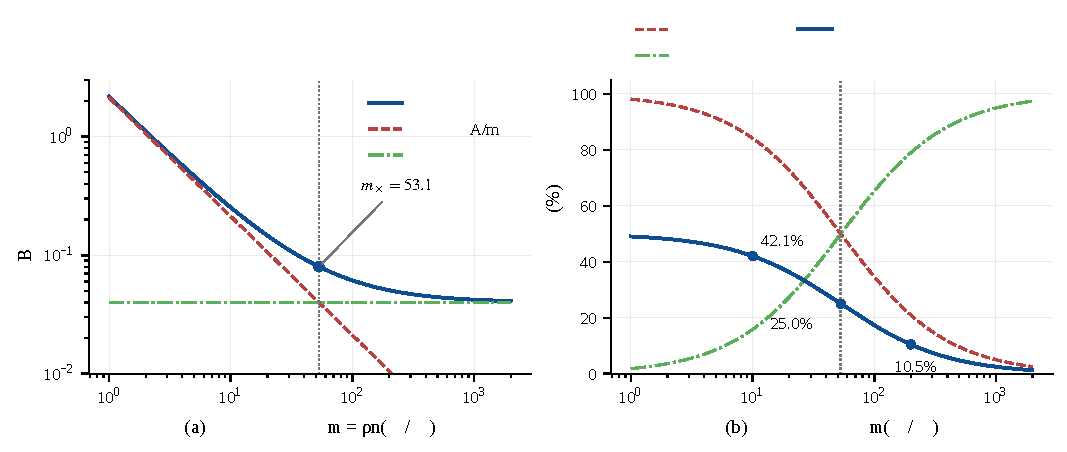
\includegraphics[width=0.95\linewidth]{figures/fig_variance_scale.pdf}
\caption{论文图 1 参数（$\bar R=1.15$，$v_R=0.04$，$k=0.35$，$\rho=0.25$）下目标 B 的单期方差随期望报告规模 $m=\rho n$ 的变化。左图在对数坐标下画出总方差 $v_R+A/m$、规模项 $A/m$ 与环境下限 $v_R$，二者在交叉点 $m_\times=53.1$ 相交，此处总方差为 $2v_R$。右图给出规模项占比、环境项占比以及规模翻倍带来的方差降幅，降幅在 $m=10$、$m_\times$、$m=200$ 处分别为 42.1\%、25.0\%、10.5\%，恒等于规模项占比的一半。}
\label{fig:pa-variance}
\end{figure}

图~\ref{fig:pa-variance} 左图中总方差曲线在小规模端贴着斜率 $-1$ 的规模项，在大规模端趋平于 $v_R$，中间平滑过渡，看不到任何折点，这正是第 4 步“严格凸、无拐点”的图形表现。右图中翻倍降幅曲线与规模项份额曲线处处相差一半，对应式~(\ref{eq:pa-halving})。

\subsubsection{与仿真和实证的对应}

原文图 1(c) 展示误差预算的演变，并标出在 $m_\times=53.1$ 处两项各占 50\%（原文第 196 行）。我们的核验确认 $A=2.1232$、$m_\times=53.08$，$m=m_\times$ 处环境项份额精确为 $1/2$，导数与翻倍降幅公式符号成立；表~\ref{tab:pa-mc2} 最后一列显示蒙特卡洛估计的环境项份额在 $m=1,10,53,500$ 处为 0.019、0.159、0.499、0.904，与理论值 0.018、0.159、0.500、0.904 一致。原文图 3(c) 与第 399、409 行报告的翻倍降幅 42.1\%、25.0\%、10.5\% 与精确值 42.07\%、25.00\%、10.49\% 一致；同一图中更新过程的经验降幅在 $m<12$ 段系统性高于解析式（$m=6\to12$ 为 73.5\%），这一偏离属于更新过程的额外误差，不影响定义 1 本身的代数。

实证部分用 $m_\times^{\mathrm{emp}}=b/a=2.2434/0.0991=22.6$ 与流感住院情景区间 21.3--49.3（原文第 515 行）比较。情景区间上端按一致参数应为 49.18。更关键的是，分母由报告病例构造时二项噪声会放大斜率：在原始滞后权重下，含噪分母使 $b/a$ 的期望由真实的 30.7 升到 59.2。实证中截距也被放大，两者部分抵消，所以“同一量级”不能当作 $m_\times$ 的结构性验证，详见第~\ref{sec:empirical} 节。

\subsubsection{原文表述的问题}

第一，原文第 187 行和图 1(c) 图注把 $m_\times$ 称为“收益拐点”。由第 4 步，$V$ 严格凸，没有拐点；$m_\times$ 是弹性等于 $-1/2$、两项份额各半的刻度。建议全文统一称“方差占比交叉点”，并在第 190 行补上弹性 $-m_\times/(m+m_\times)$，这比“导数平滑连续、不存在突变”更能说明交叉点的经济含义。

第二，原文图 1(c) 中交叉点的标注在 PDF 中渲染为“m imes”，是乘号命令的转义错误，应在作图脚本中修正。

\subsection{命题 3：扩大基数与提高报告率}

\subsubsection{原式与参数含义}

论文为比较两条增加报告病例的政策路径，把原文式 7 写成 $(n,\rho)$ 的二元函数，如下式所示：
\begin{equation*}
V(n, \rho) = v_R + \frac{\bar{R}}{\rho n} + \frac{\bar{R}^2 + v_R}{k n}.
\tag{原文式 10}
\end{equation*}
为分离报告率的作用，论文把第二项恒等拆分为完全报告时的计数项与漏报项，如下式所示：
\begin{equation*}
\frac{\bar{R}}{\rho n} = \frac{\bar{R}}{n} + \frac{(1-\rho)\bar{R}}{\rho n}.
\tag{原文式 11}
\end{equation*}
命题 3 第 (i) 条给出报告率趋于 1 时的饱和下界，原式如下：
\begin{equation*}
\lim_{\rho \to 1} V(n, \rho) = v_R + \frac{\bar{R}}{n} + \frac{\bar{R}^2 + v_R}{k n} > v_R.
\tag{原文式 12}
\end{equation*}
命题 3 第 (ii) 条给出风险集规模趋于无穷时的极限，原式如下：
\begin{equation*}
\lim_{n \to \infty} V(n, \rho) = v_R.
\tag{原文式 13}
\end{equation*}

\begin{itemize}
\item $n$ 是真实风险集规模，取正整数，求极限时把它看成可以连续增大的量；扩大 $n$ 对应扩大哨点覆盖或跨区域汇总感染者。
\item $\rho$ 是报告率，取值于 $(0,1]$；提高 $\rho$ 对应加强筛查、降低检测门槛。
\item $\bar R/n$ 是完全报告时仍存在的 Poisson 计数波动，$(1-\rho)\bar R/(\rho n)$ 是漏报额外引入的抽样方差，$(\bar R^2+v_R)/(kn)$ 是个体超传播造成的子代抽样方差。
\item $v_R$、$\bar R$、$k$ 的含义同命题 2，在命题 3 中都视为固定。
\end{itemize}

\subsubsection{逐步推导}

\begin{enumerate}
\item 由原文式 7 把 $n$ 与 $\rho$ 分开书写即得原文式 10，它在数值上就是命题 2 的方差，没有新增假设。
\item 由通分可验证原文式 11：右端为 $[\rho\bar R+(1-\rho)\bar R]/(\rho n)=\bar R/(\rho n)$。
\item 对原文式 10 关于 $\rho$ 求偏导，只有第二项含 $\rho$，得 $\partial V/\partial\rho=-\bar R/(\rho^2n)<0$；因此 $V$ 关于 $\rho$ 严格递减，而超传播项 $(\bar R^2+v_R)/(kn)$ 与 $\rho$ 无关，提高 $\rho$ 对它没有作用。
\item 由 $V$ 关于 $\rho$ 的连续性取 $\rho\to1$，漏报项 $(1-\rho)\bar R/(\rho n)\to0$，得到原文式 12 的等号部分；由于 $n<\infty$，$\bar R/n$ 与 $(\bar R^2+v_R)/(kn)$ 都严格为正，所以极限严格大于 $v_R$。结合第 3 步的单调性，这个极限值也是 $V$ 在 $\rho\in(0,1]$ 上的最小值，等于 $V(n,1)$。
\item 对原文式 10 关于 $n$ 求偏导得 $\partial V/\partial n=-[\bar R/\rho+(\bar R^2+v_R)/k]/n^2<0$；由 $1/n\to0$，后两项都是 $O(1/n)$，对任意固定的 $\rho\in(0,1]$ 都趋于零，得到原文式 13。
\item 由 $n=m/\rho$ 把原文式 10 改写为 $(m,\rho)$ 的函数
\begin{equation*}
V=v_R+\frac{\bar R}{m}+\frac{\rho(\bar R^2+v_R)}{km},
\end{equation*}
可见固定 $m$ 时提高 $\rho$ 等于缩小 $n$，超传播项反而变大；这就是原文第 187 行所说“$A$ 依赖 $\rho$”与命题 3 非对称性的同一来源。
\item 命题 3 只比较了极限，政策上更有用的是边际比较：让 $m$ 增加同样的比例，一次沿 $n$、一次沿 $\rho$。由对数求导 $\partial V/\partial\ln n=n\,\partial V/\partial n$，沿 $n$ 方向得 $\partial V/\partial\ln n=-\bar R/(\rho n)-(\bar R^2+v_R)/(kn)=-A/m$。
\item 同理沿 $\rho$ 方向只有第二项变化，得 $\partial V/\partial\ln\rho=\rho\,\partial V/\partial\rho=-\bar R/(\rho n)=-\bar R/m$。
\item 由 $\mathrm d\ln m=\mathrm d\ln n$（固定 $\rho$）或 $\mathrm d\ln m=\mathrm d\ln\rho$（固定 $n$），把第 7、8 步相除，得到每增加 1\% 的期望报告规模时两条路径的方差降幅之比
\begin{equation}
\frac{\partial V/\partial\ln n}{\partial V/\partial\ln\rho}=\frac{A}{\bar R}=1+\frac{\rho(\bar R^2+v_R)}{k\bar R}.
\label{eq:pa-margratio}
\end{equation}
它恒大于 1，且随 $\rho$、$v_R$ 增大而增大，随 $k$ 增大而减小。
\end{enumerate}

\subsubsection{直觉与数值例}

回到式~(\ref{eq:pa-relvar})，报告病例的相对方差由 $1/(\rho nR_t)$ 与 $1/(nk)$ 组成。超传播噪声 $1/(nk)$ 只与真实感染者数 $n$ 有关：子代数的离散发生在传播环节，报告只是在已经实现的感染者中抽样，报告得再完整也只能看清这份离散，无法消除它。提高 $\rho$ 最多把报告尺度的计数噪声 $\bar R/(\rho n)$ 压到完全报告时的 $\bar R/n$；扩大 $n$ 则同时压缩全部三项规模相关方差。

取论文图 1 参数，从 $n=40$、$\rho=0.25$（$m=10$）出发，$V=0.25232$，其中 $v_R=0.04$，计数项 $\bar R/n=1.15/40=0.02875$，漏报项 $(1-\rho)\bar R/(\rho n)=0.08625$，超传播项 $0.09732$。把报告率提到 1（$m=40$），只能去掉漏报项，$V=0.04+0.02875+0.09732=0.16607$。把 $n$ 扩大到 160 而保持 $\rho=0.25$（同样 $m=40$），$V=0.04+2.12321/40=0.09308$。两条路径把 $m$ 提到同一水平，方差相差 $0.07299$，这正是超传播项从 $0.09732$ 降到 $0.02433$ 的部分。

式~(\ref{eq:pa-margratio}) 给出边际比较。图 1 参数下 $A/\bar R=1+0.340625/(0.35\times1.15)=1+0.340625/0.4025=1.846$，扩大基数的边际效果是提高报告率的 1.85 倍。流感住院情景（$\bar R=1.67$，$k\in[0.2,0.5]$，$\rho\in[0.0056,0.021]$，$v_R\in[0.04,0.08]$，原文第 515 行）下，由第 9 步的单调性，下端取 $\rho=0.0056$、$k=0.5$、$v_R=0.04$，得 $1+0.0056\times2.8289/(0.5\times1.67)=1.019$；上端取 $\rho=0.021$、$k=0.2$、$v_R=0.08$，得 $1+0.021\times2.8689/(0.2\times1.67)=1.180$。住院监测的报告率很低，两条路径的边际效果只差 2\%--18\%。

\subsubsection{与仿真和实证的对应}

原文图 1 只用一个报告率 $\rho=0.25$，没有直接仿真命题 3 的两条路径。我们的符号核验确认恒等拆分、$\rho\to1$ 极限、$n\to\infty$ 极限以及式~(\ref{eq:pa-margratio}) 全部成立；流感住院情景下的边际比 $[1.019,1.180]$ 被判为“偏差”，意思是结论方向成立而数量上很弱。

实证部分把医院填报覆盖率当作 $\rho$ 的制度层面代理（原文第 467 行），并把 2024 年强制报告到自愿填报的切换作为命题 3 的对照场景（原文第 613 行）：覆盖率由 91.1\% 降到 54.6\%，观测增长率的离散程度由 0.624 升到 1.823，扩大约 2.92 倍。若覆盖率下降只是均匀的二项漏报，离散程度至多放大 $\sqrt{0.911/0.546}=1.29$ 倍，实测远超这一上界，支持论文“结构性非随机扰动”的解释，也说明 2024 年的覆盖率冲击与命题 3 只能建立定性联系。原文第 617 行的全国汇总看起来对应“扩大 $n$”，但它压低误差的主要机制是削减跨州不完全相关的环境方差，命题 3 的 $n\to\infty$ 极限仍停在 $v_R$，二者的对应见命题 2 的讨论。

\subsubsection{原文表述的问题}

第一，命题 3 只比较极限就称两条杠杆存在“本质非对称性”，而原文第 467、613、658 行把它作为住院数据实证与政策结论的理论依据。由式~(\ref{eq:pa-margratio})，非对称的大小正比于 $\rho/k$，在住院情景下边际比只有 1.02--1.18，两条路径近似等价；非对称性在高报告率、强超传播的场景（如接触者追踪）中才有实际意义。建议在命题 3 后加一条注记给出 $A/\bar R$，并在上述三处注明住院情景下非对称性在数量上很弱。

第二，命题 3 第 (ii) 条与原文第 168 行一样默认所有感染者共享同一环境，所以 $n\to\infty$ 时方差停在 $v_R$；第 617 行跨州汇总突破单州下限，依靠的是环境不完全相关，与命题 3 的机制不同。两处应统一表述，避免答辩时被指出前后矛盾。

第三，由第 4 步，$\rho=1$ 本身属于参数空间，原文式 12 的极限可以直接写成函数值 $V(n,1)$，并说明它是 $V$ 关于 $\rho$ 的最小值；用“极限”表述没有错，改写为“最小值”更直接。

% 第 4 章下半部分：命题 4、推论 1、命题 5、命题 6 与更新过程仿真中的恒等式
% label 前缀 pb-

\subsection{命题 4：预算约束下的期数与规模}

\subsubsection{原式与参数含义}

命题 4 回答的问题是在总监测规模固定时，预算应当分给更多的观测期，还是分给更大的单期规模。原文第 237 行设定了一个理想化的重复采样设计。设计者在 $T$ 个观测期内设定相同的每期真实风险集规模 $n_T=B/(\rho T)$，记设计方案为 $\mathcal D_T=(T,n_T)$，并假定 $\bar R$、$\rho$、$k$、$v_R$ 不随期变化。给定完整环境扰动序列后，各期的分支传播与报告抽样相互条件独立。跨期基础水平 $\bar R$ 的估计量取各期矩估计量的样本平均，原文的定义如下式所示：
\begin{equation*}
\overline{\widehat{R}}_T \triangleq \frac{1}{T} \sum_{t=1}^T \widehat{R}_t = \frac{1}{T} \sum_{t=1}^T \frac{C_t}{\rho n_T}.
\tag{原文式 14}
\end{equation*}

命题 4（原文第 244–263 行）共有三条结论。第 (i) 条在环境扰动跨期独立时给出平均估计量的精确方差，如下式所示：
\begin{equation*}
\operatorname{Var}(\overline{\widehat{R}}_T \mid n_T) = \frac{v_R}{T} + \frac{A}{B},
\tag{原文式 15}
\end{equation*}
第 (ii) 条在环境扰动服从一阶自回归时给出有效独立期数形式的近似，如下式所示：
\begin{equation*}
\operatorname{Var}(\overline{\widehat{R}}_T \mid n_T) \approx \frac{v_R}{T_{\operatorname{eff}}(T, r)} + \frac{A}{B}, \qquad T_{\operatorname{eff}}(T, r) \triangleq T \frac{1-r}{1+r},
\tag{原文式 16}
\end{equation*}
第 (iii) 条给出严格用尽预算且各期风险集为相同正整数时可供比较的期数集合，如下式所示：
\begin{equation*}
\mathcal{T}(B, \rho) \triangleq \left\{ T \in \mathbb{N}_+ \;:\; \frac{B}{\rho T} \in \mathbb{N}_+ \right\}.
\tag{原文式 17}
\end{equation*}

附录对第 (ii) 条给出了有限期数下的精确双重求和闭式，它是本节推导的核心，原文写法如下：
\begin{equation*}
\operatorname{Var}\left(\sum_{t=1}^T R_t \;\middle|\; n_T\right) = T v_R + 2 v_R \sum_{s=1}^{T-1} (T-s) r^s = v_R T \left[\frac{1+r}{1-r} - \frac{2r(1-r^T)}{T(1-r)^2}\right].
\tag*{原文第 751 行}
\end{equation*}

各式中出现的参数含义如下。
\begin{itemize}
\item $T$ 是观测期数，取正整数，在命题 4 中是设计者可以选择的变量。
\item $n_T$ 是每期上一代真实风险集人数，只有取正整数时才对应一个可以实施的设计。
\item $\rho\in(0,1]$ 是报告率，即每个真实感染最终被报告的概率。
\item $m=\rho n_T$ 是每期期望被报告规模，单位为例/期，与第~\ref{sec:model} 节定义的 $m$ 相同。
\item $B=Tm$ 是总监测输入规模，即各期期望被报告人数之和，单位为例；它与推论 1 中以货币计的总经费 $\mathcal B$ 是两个不同的量。
\item $C_t$ 是第 $t$ 期的报告病例数，$\widehat R_t=C_t/(\rho n_T)$ 是第 $t$ 期的矩估计量，命题 1 已证明它同时是极大似然估计量且条件无偏。
\item $\bar R>0$ 是跨期基础传播水平，$v_R=\operatorname{Var}(R_t)\ge 0$ 是环境方差，$k>0$ 是个体离散参数。
\item $A=\bar R+\rho(\bar R^2+v_R)/k$ 是命题 2 的方差系数；原文第 251 行特意说明它与估计目标“目标 A”同名而含义不同。
\item $r\in[0,1)$ 是环境扰动的一阶自回归系数，满足 $\operatorname{Cov}(R_t,R_{t+s}\mid n_T)=v_Rr^{|s|}$；它与命题 6 中负二项累积分布函数 $F_{\operatorname{NB}}(x;r,p)$ 的形状参数同名，后者取 $r=nk$，两者无关。
\item $T_{\operatorname{eff}}(T,r)$ 是有效独立期数，$\mathcal T(B,\rho)$ 是可行期数集合，$\mathbb N_+$ 是正整数集合。
\end{itemize}

\subsubsection{逐步推导}

第 (i) 条的推导以整条环境序列 $\{R_t\}$ 为条件，分七步完成。
\begin{enumerate}
\item 由原文第 238 行的设计假定，给定 $\{R_t\}$ 后各期相互条件独立；再由命题 1 的条件无偏性 $\mathbb E[\widehat R_t\mid R_t,n_T]=R_t$，内层条件期望为 $\mathbb E[\overline{\widehat R}_T\mid\{R_t\},n_T]=\frac1T\sum_{t=1}^TR_t$。
\item 以 $\{R_t\}$ 为条件应用全方差公式（附录引理~\ref{lem:ap-totvar}），总方差拆成两项：
\begin{equation*}
\operatorname{Var}(\overline{\widehat R}_T\mid n_T)=\operatorname{Var}\Big(\frac1T\sum_{t=1}^TR_t\;\Big|\;n_T\Big)+\mathbb E\big[\operatorname{Var}(\overline{\widehat R}_T\mid\{R_t\},n_T)\,\big|\,n_T\big].
\end{equation*}
\item 由方差的二次齐次性 $\operatorname{Var}(cY)=c^2\operatorname{Var}(Y)$，第一项等于 $T^{-2}\operatorname{Var}(\sum_tR_t\mid n_T)$。
\item 由条件独立随机变量之和的方差等于各自方差之和，内层条件方差为 $T^{-2}\sum_t\operatorname{Var}(\widehat R_t\mid R_t,n_T)$；代入命题 1 的条件方差（原文式 6）得到每一期的条件方差为 $R_t/(\rho n_T)+R_t^2/(kn_T)$。
\item 对每一期取期望时使用二阶矩关系 $\mathbb E[R_t^2]=\bar R^2+v_R$（原文第 728 行），得 $\bar R/(\rho n_T)+(\bar R^2+v_R)/(kn_T)$；再以 $1/n_T=\rho/m$ 代换，它等于 $\frac1m[\bar R+\rho(\bar R^2+v_R)/k]=A/m$，这一步与命题 2 把原文式 7 改写为 $v_R+A/m$ 的过程完全相同。
\item 把 $T$ 个相同的 $A/m$ 相加再除以 $T^2$，第二项等于 $A/(Tm)$，也就是附录第 743–747 行第三行中的 $A/(T\rho n_T)$；用预算约束 $Tm=B$ 代换后第二项等于 $A/B$，与 $T$ 无关。
\item 环境跨期独立时，独立变量和的方差可加，$\operatorname{Var}(\sum_tR_t)=Tv_R$，第一项等于 $v_R/T$；两项相加即得原文式 15，而对 $T$ 求导得 $-v_R/T^2<0$，所以固定 $B$ 时增加 $T$ 严格降低方差。
\end{enumerate}

第 (ii) 条需要计算相关随机变量之和的方差。附录用错位相减完成这一步，下面给出一条按行求和的路线，每一步都只用到有限等比级数。
\begin{enumerate}
\item 由方差的双线性展开，得到下式：
\begin{equation*}
\operatorname{Var}\Big(\sum_{t=1}^T R_t\Big)=\sum_{t=1}^T\sum_{u=1}^T\operatorname{Cov}(R_t,R_u).
\end{equation*}
再代入一阶自回归过程的自协方差 $\operatorname{Cov}(R_t,R_u)=v_Rr^{|t-u|}$ \citep{hamilton1994time}，所求方差等于一个 $T\times T$ 矩阵全部元素之和。
\item 按间隔 $s=|t-u|$ 分组计数：对角线上 $s=0$ 的元素有 $T$ 个，每个等于 $v_R$；间隔为 $s\ge1$ 的有序对在上三角与下三角各有 $T-s$ 个，共 $2(T-s)$ 个，于是得到附录闭式的第一个等号
\begin{equation}
\operatorname{Var}\Big(\sum_{t=1}^TR_t\Big)=Tv_R+2v_R\sum_{s=1}^{T-1}(T-s)r^s .\label{eq:pb-sumcov}
\end{equation}
\item 式~\eqref{eq:pb-sumcov} 中的级数等于上三角元素（除以 $v_R$）之和；按行计算，第 $t$ 行对角线右侧有 $j=T-t$ 个元素，由有限等比级数公式其和为 $r+r^2+\dots+r^j=r(1-r^j)/(1-r)$，再对 $j=1,\dots,T-1$ 求和并对 $\sum_{j=1}^{T-1}r^j$ 再用一次等比级数公式，得
\begin{equation*}
\sum_{s=1}^{T-1}(T-s)r^s=\sum_{j=1}^{T-1}\frac{r(1-r^j)}{1-r}=\frac{r(T-1)}{1-r}-\frac{r^2(1-r^{T-1})}{(1-r)^2}.
\end{equation*}
\item 通分化简时把 $\frac{r(T-1)}{1-r}$ 拆成 $\frac{rT}{1-r}-\frac{r(1-r)}{(1-r)^2}$，与第二项合并后分子为 $r(1-r)+r^2-r^{T+1}=r(1-r^T)$，于是
\begin{equation*}
\sum_{s=1}^{T-1}(T-s)r^s=\frac{rT}{1-r}-\frac{r(1-r^T)}{(1-r)^2}.
\end{equation*}
\item 代回式~\eqref{eq:pb-sumcov} 并利用恒等式 $1+\frac{2r}{1-r}=\frac{1+r}{1-r}$，得 $Tv_R+\frac{2v_RrT}{1-r}-\frac{2v_Rr(1-r^T)}{(1-r)^2}=v_RT\big[\frac{1+r}{1-r}-\frac{2r(1-r^T)}{T(1-r)^2}\big]$，这就是附录第 751 行的第二个等号。
\item 把闭式除以 $T^2$，得到 AR(1) 环境下平均估计量环境项的精确表达
\begin{equation}
\operatorname{Var}\Big(\frac1T\sum_{t=1}^TR_t\Big)=\frac{v_R}{T}\Big[\frac{1+r}{1-r}-\frac{2r(1-r^T)}{T(1-r)^2}\Big],\label{eq:pb-exactenv}
\end{equation}
总方差等于式~\eqref{eq:pb-exactenv} 加上与 $r$ 无关的 $A/B$，因为第 (i) 条第 4–6 步只用到给定 $\{R_t\}$ 时的条件独立性，与环境序列的相关结构无关。
\item 原文式 16 相当于丢掉方括号中的第二项，此时环境项变为 $\frac{v_R}{T}\cdot\frac{1+r}{1-r}=v_R/T_{\operatorname{eff}}$；由于 $0\le r<1$ 时 $1-r^T>0$，被丢掉的项非负且在 $r>0$ 时严格为正，所以该近似对环境项恒高估，等价于恒低估有效期数。
\item 用近似值除以精确值再减 1，并把分子分母同乘 $T(1-r)^2$，得到相对高估比例的闭式
\begin{equation}
\frac{\text{近似环境项}}{\text{精确环境项}}-1=\frac{2r(1-r^T)}{T(1-r)(1+r)-2r(1-r^T)} .\label{eq:pb-overrate}
\end{equation}
\item 当 $T$ 增大时 $r^T\to0$，且分母中的 $2r(1-r^T)$ 相对 $T(1-r^2)$ 可以忽略，由此得到式~\eqref{eq:pb-overrate} 的一阶近似 $2r/[T(1-r^2)]$；它说明相对误差只以 $1/T$ 的速度衰减，误差的刻度是 $2r/(1-r^2)$ 期，$r=0.8$ 时约为 4.44 期。
\end{enumerate}

第 (iii) 条只涉及整除关系，推导分三步。
\begin{enumerate}
\item 由 $m=\rho n_T$ 与 $B=Tm$ 联立解出 $n_T=B/(\rho T)$，所以 $B/\rho=Tn_T$。
\item 若要求 $n_T\in\mathbb N_+$，则 $B/\rho$ 是正整数 $T$ 与正整数 $n_T$ 的乘积，必须是正整数；因此当 $B/\rho\notin\mathbb N_+$ 时可行集为空，当 $B/\rho\in\mathbb N_+$ 时条件等价于 $T$ 整除 $B/\rho$，可行集就是 $B/\rho$ 的全部正因子。
\item 由于正整数的任何正因子都不超过它本身，$T\le\lfloor B/\rho\rfloor$ 是属于 $\mathcal T(B,\rho)$ 的必要条件，但满足该不等式而不整除 $B/\rho$ 的 $T$ 仍不可行，所以它只是必要条件，充分性不成立。
\end{enumerate}

\subsubsection{直觉与数值例}

总报告数一定时，抽样噪声只取决于报告总数，这是负二项计数在独立相加下方差可加的直接结果，所以 $A/B$ 与切分方式无关；环境噪声则只能靠增加期数来平均。纯人数预算下的最优设计因此是把期数拉到最大，而无限多期在现实中不可行，推论 1 引入每期固定成本 $c_0$ 正是为了修正这一点。

取论文图 1 参数 $\bar R=1.15$、$v_R=0.04$、$k=0.35$、$\rho=0.25$，此时 $A=1.15+0.25\times(1.3225+0.04)/0.35=2.1232$。设总规模 $B=260$ 例，比较两种设计。
\begin{itemize}
\item 设计一为 $T=10$、$m=26$：环境项 $v_R/T=0.004$，抽样项 $A/B=2.1232/260=0.008166$，独立环境下总方差为 $0.01217$。
\item 设计二为 $T=26$、$m=10$：环境项 $0.04/26=0.001538$，抽样项仍为 $0.008166$，总方差为 $0.00970$。两种设计的抽样项完全相同，差别全部来自环境项。
\item 若环境自相关 $r=0.8$，设计一的方括号为 $9-1.6\times(1-0.8^{10})/(10\times0.04)=9-3.5705=5.4295$，由式~\eqref{eq:pb-exactenv} 得精确环境项 $0.004\times5.4295=0.02172$，总方差 $0.02988$；而原文式 16 给出环境项 $0.004\times9=0.036$，总方差 $0.04417$。环境项被高估 65.8\%。
\item 同样在 $r=0.8$ 下，设计二的精确总方差为 $0.01965$，近似值为 $0.02201$。按式~\eqref{eq:pb-overrate}，分子 $1.6\times(1-0.8^{26})=1.5952$，分母 $26\times0.2\times1.8-1.5952=7.7648$，环境项高估 20.5\%；对应的精确有效期数为 3.48，而 $T_{\operatorname{eff}}=26\times0.2/1.8=2.89$。
\end{itemize}

图~\ref{fig:pb-ar1} 给出式~\eqref{eq:pb-overrate} 在 $T=8$ 到 80 上的完整曲线。$r=0.3$ 与 $r=0.5$ 时高估幅度在 $T\ge20$ 后已降到个位数，$r=0.8$ 时曲线下降缓慢，$T=80$ 仍有数个百分点。若要求环境项误差不超过 5\%，在 $r=0.8$ 下按一阶近似约需 $T\approx89$，按精确式需 $T=94$。

\begin{figure}[!tbp]\centering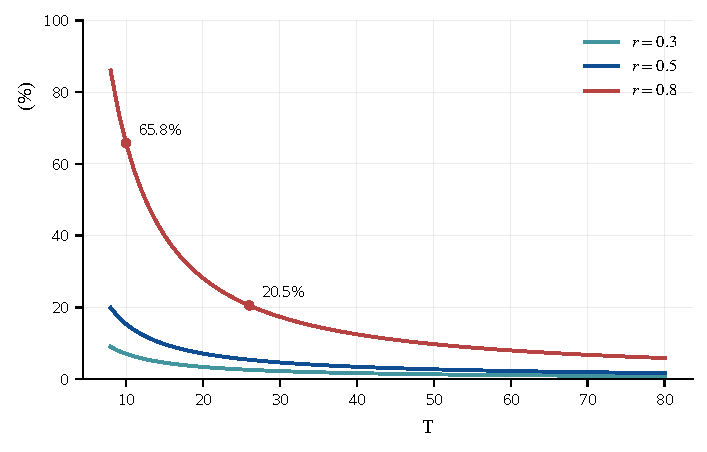
\includegraphics[width=0.62\linewidth]{figures/fig_ar1_teff.pdf}\caption{有效期数近似 $T_{\operatorname{eff}}=T(1-r)/(1+r)$ 对环境方差项的相对高估幅度。横轴为观测期数 $T$，纵轴为近似值相对附录精确闭式的高估百分比，三条曲线对应 $r=0.3$、$0.5$、$0.8$；$r=0.8$ 时 $T=10$ 高估 65.8\%，$T=26$ 仍高估 20.5\%。}\label{fig:pb-ar1}\end{figure}

可行集的三个例子如下。$B=30$、$\rho=0.25$ 时 $B/\rho=120$，可行期数是 120 的 16 个正因子 $\{1,\allowbreak 2,\allowbreak 3,\allowbreak 4,\allowbreak 5,\allowbreak 6,\allowbreak 8,\allowbreak 10,\allowbreak 12,\allowbreak 15,\allowbreak 20,\allowbreak 24,\allowbreak 30,\allowbreak 40,\allowbreak 60,\allowbreak 120\}$；$B=30$、$\rho=0.7$ 时 $B/\rho=42.86$ 带有小数部分，可行集为空；$T=7$ 满足 $7\le120$，但 7 不整除 120，所以不可行。

\subsubsection{与仿真和实证的对应}

论文的图 1–3 都没有直接检验命题 4，正文第 264–269 行只给出机制解释。本讲义的核验分三层完成。
\begin{itemize}
\item 符号核验确认了第 (i) 条的全方差推导与 $\partial/\partial T=-v_R/T^2$，并在 $T=1,\dots,40$ 上逐个确认式~\eqref{eq:pb-sumcov} 的级数与按行求和闭式恒等，附录第 751 行的两个等号均成立。
\item 蒙特卡洛核验在图 1 参数下比较了 $T=10$、$m=26$（20000 次重复）与 $T=26$、$m=10$（7692 次重复）两种设计、$r\in\{0,0.5,0.8\}$ 六种情形。模拟方差与精确闭式全部在 $|z|<3$ 内一致，例如 $T=10$、$r=0.8$ 时模拟值 0.02998 对精确值 0.02988（$z=0.33$），$T=26$、$r=0.8$ 时 0.01895 对 0.01965（$z=-2.31$）；同一情形下原文式 16 的近似值 0.04417 与 0.02201 明显偏离模拟值。
\item 在 $r\in[0,0.98]$、$T\le300$ 的网格上，式~\eqref{eq:pb-exactenv} 关于 $T$ 严格递减，所以命题 4(i) 中“增加 $T$ 严格降低方差”的结论在 AR(1) 环境下仍然成立，这一点论文没有说明。
\end{itemize}
可行集的三个例子（120 的 16 个正因子、空集、$T=7$ 的反例）也逐一得到确认。实证部分（第~\ref{sec:empirical} 节）没有估计周增长比的自相关系数，所以 $r$ 的取值在本文中仍是情景参数。

\subsubsection{原文表述的问题}

\begin{itemize}
\item 第 254–256 行称在 $T\gg1/(1-r)$ 时原文式 16 是“良好近似”，但没有说明近似方向。由第 7 步，近似恒高估环境项，从设计角度看偏保守；$T=26$、$r=0.8$ 时 $T(1-r)=5.2$，已大于 $1/(1-r)=5$，误差仍有 20.5\%。附录第 753 行说丢掉的是 $O(1/T^2)$ 项，这在绝对量上成立，但相对主项只是 $O(1/T)$。建议正文直接写出附录第 751 行的精确闭式（它本身就是初等函数），把 $T_{\operatorname{eff}}$ 作为直觉保留，并写明近似方向。
\item 方差系数 $A$ 与“目标 A”同名，AR(1) 系数 $r$ 与负二项形状参数 $r=nk$ 同名，答辩时容易被追问，建议改记方差系数为 $\kappa$、AR(1) 系数为 $\phi$，或把两类估计目标改称“目标 I”“目标 II”。
\end{itemize}

\subsection{推论 1：成本最优的单期规模}

\subsubsection{原式与参数含义}

推论 1 在命题 4 的基础上引入两类成本：每个观测期的固定运转成本 $c_0>0$，以及每捕获一个报告病例的边际成本 $c_1>0$。原文第 274 行给出的总经费约束如下：
\begin{equation*}
\mathcal{B} = T(c_0 + c_1 m)
\tag*{原文第 274 行}
\end{equation*}
同一行给出的待最小化目标函数如下：
\begin{equation*}
\operatorname{Var}(\overline{\widehat{R}}_T) = \frac{v_R}{T} + \frac{A}{T m}
\tag*{原文第 274 行}
\end{equation*}
推论 1 的结论是唯一内部最优单期规模，原文写法如下：
\begin{equation*}
m^* = \sqrt{\frac{c_0}{c_1} \cdot \frac{A}{v_R}} = \sqrt{\frac{c_0}{c_1} m_\times}.
\tag{原文式 18}
\end{equation*}
若内部解超出可行上界，原文第 279 行给出的角点解如下：
\begin{equation*}
m^* = \frac{\mathcal{B} - c_0}{c_1}
\tag*{原文第 279 行}
\end{equation*}
原文第 280 行在 AR(1) 环境下先把环境方差替换为有效环境方差：
\begin{equation*}
v_{\mathrm{eff}} \approx v_R \frac{1+r}{1-r}
\tag*{原文第 280 行}
\end{equation*}
并由此给出修正后的最优单期规模：
\begin{equation*}
m^*_{\mathrm{AR}} \approx \sqrt{\frac{c_0}{c_1} m_\times \frac{1-r}{1+r}} < m^*
\tag*{原文第 280 行}
\end{equation*}

各式中出现的参数含义如下。
\begin{itemize}
\item $c_0>0$ 是每个观测期的固定成本，例如哨点的运转与维持开销，单位为货币/期。
\item $c_1>0$ 是每个报告病例的边际成本，单位为货币/例；若按覆盖人群计的人均成本为 $c_1'$，覆盖 $n$ 人的花费 $c_1'n=c_1'm/\rho$，所以 $c_1=c_1'/\rho$。
\item $\mathcal B>0$ 是总经费预算；为保证 $T\ge1$，单期规模须满足 $m\le(\mathcal B-c_0)/c_1$。
\item $T\ge1$ 是期数，推论中先按连续变量处理；$m>0$ 是单期期望报告规模。
\item $m_\times=A/v_R$ 是定义 1 的方差占比交叉点，图 1 参数下 $m_\times=53.08$。
\item $v_{\mathrm{eff}}$ 是 AR(1) 环境下的有效环境方差，$m^*_{\mathrm{AR}}$ 是相应的近似最优规模，$r\in[0,1)$ 的含义同命题 4。
\end{itemize}

\subsubsection{逐步推导}

\begin{enumerate}
\item 由预算约束解出 $T=\mathcal B/(c_0+c_1m)$，代入目标函数 $\frac1T(v_R+A/m)$，展开乘积后得到只含 $m$ 的一元函数
\begin{equation}
f(m)=\frac{(c_0+c_1m)(v_R+A/m)}{\mathcal B}=\frac{c_0v_R+c_0A/m+c_1v_Rm+c_1A}{\mathcal B}.\label{eq:pb-fm}
\end{equation}
\item 由幂函数求导法则对式~\eqref{eq:pb-fm} 逐项求导，常数项 $c_0v_R$ 与 $c_1A$ 的导数为零，得 $f'(m)=(c_1v_R-c_0A/m^2)/\mathcal B$。
\item 再求一次导数得 $f''(m)=2c_0A/(\mathcal Bm^3)$，它在 $m>0$ 上恒正，所以 $f$ 在 $(0,\infty)$ 上严格凸，一阶条件的正根若存在就是唯一的全局最小点，这就是原文第 275 行二阶导的含义。
\item 令 $f'(m)=0$ 得 $m^2=c_0A/(c_1v_R)$，取正根，并代入定义 1 的 $m_\times=A/v_R$，即得原文式 18。
\item 把 $m^*$ 代回式~\eqref{eq:pb-fm}，由 $m^{*2}=c_0A/(c_1v_R)$ 可得两个随 $m$ 变化的项相等，$c_0A/m^*=c_1v_Rm^*=\sqrt{c_0c_1Av_R}$；再用完全平方公式合并，最小方差为
\begin{equation}
f(m^*)=\frac{c_0v_R+c_1A+2\sqrt{c_0c_1Av_R}}{\mathcal B}=\frac{\big(\sqrt{c_0v_R}+\sqrt{c_1A}\big)^2}{\mathcal B}.\label{eq:pb-fmin}
\end{equation}
\item 同一结果也可以由算术–几何平均不等式 $c_0A/m+c_1v_Rm\ge2\sqrt{c_0c_1Av_R}$ 直接读出，取等条件 $c_0A/m=c_1v_Rm$ 正是第 4 步的一阶条件。
\item 若把 $T$ 与 $m$ 都当作连续变量并用 Lagrange 乘子法，令 $u=1/T$，在约束 $c_0+c_1m=\mathcal Bu$ 下最小化 $u(v_R+A/m)$，对 $u$ 与 $m$ 的一阶条件分别为 $v_R+A/m=\lambda\mathcal B$ 与 $uA/m^2=\lambda c_1$；消去 $\lambda$ 后得 $c_1(v_R+A/m)=(c_0+c_1m)A/m^2$，即 $c_1v_R=c_0A/m^2$，与代入法一致。
\item 可行性 $T\ge1$ 等价于 $m\le(\mathcal B-c_0)/c_1$；由于凸函数 $f$ 在 $m^*$ 左侧单调递减，当 $m^*$ 超出这一上界时，可行域内的最小点落在上界本身，对应 $T=1$，这就是原文第 279 行的角点解。
\item 当 $c_0=0$ 时 $f'(m)=c_1v_R/\mathcal B>0$，$f$ 单调递增，最优 $m\to0$，回到命题 4 中纯人数预算下“期数越多越好”的结论。
\item 在 AR(1) 环境下，由原文式 16 有 $v_R/T_{\operatorname{eff}}=v_{\mathrm{eff}}/T$，目标函数的形式不变，只是 $v_R$ 换成 $v_{\mathrm{eff}}=v_R(1+r)/(1-r)$；重复第 1–4 步得 $m^*_{\mathrm{AR}}=\sqrt{c_0A/(c_1v_{\mathrm{eff}})}=\sqrt{(c_0/c_1)m_\times(1-r)/(1+r)}$，由于 $r>0$ 时 $(1-r)/(1+r)<1$，有 $m^*_{\mathrm{AR}}<m^*$。
\item 期数 $T$ 在实际中必须是整数；对每个整数 $T$ 取用尽预算的 $m=(\mathcal B/T-c_0)/c_1$，计算 $(v_R+A/m)/T$ 并逐一比较，即得整数约束下的最优设计，连续解 $m^*$ 只是这一枚举的下界参照。
\end{enumerate}

推论 1 与经典两阶段抽样的费用分配在数学上同构 \citep{cochran1977sampling}。Cochran 第 10 章讨论等大小初级单元的二阶抽样：抽取 $n$ 个初级单元、每个单元内抽取 $m$ 个次级单元，无限总体下估计量方差为 $S_b^2/n+S_w^2/(nm)$，总成本为 $\kappa_1n+\kappa_2nm$，最优次级样本量为 $m_{\rm opt}=\sqrt{(\kappa_1/\kappa_2)(S_w^2/S_b^2)}$。表~\ref{tab:pb-cochran} 给出逐项对应，把右列代入即得原文式 18。Cochran 在有限总体下 $S_b^2$ 的位置是 $S_1^2-S_2^2/M$，本文环境层相当于无限总体，这一位置就是 $v_R$。

\begin{table}[!tbp]\centering\small\caption{推论 1 与 Cochran 两阶段抽样的符号对应}\label{tab:pb-cochran}
\begin{tabular}{L{3.6cm}L{4.2cm}L{4.2cm}}
\toprule
Cochran 符号 & Cochran 中的含义 & 推论 1 中的对应 \\
\midrule
$n$ & 初级单元数 & 期数 $T$ \\
$m$ & 每个初级单元内的次级单元数 & 单期期望报告规模 $m$ \\
$S_b^2$ & 初级单元间方差 & 环境方差 $v_R$ \\
$S_w^2$ & 初级单元内方差 & 方差系数 $A$ \\
$\kappa_1$ & 每个初级单元的成本 & 每期固定成本 $c_0$ \\
$\kappa_2$ & 每个次级单元的成本 & 每例边际成本 $c_1$ \\
$S_w^2/S_b^2$ & 单元内外方差比 & 交叉点 $m_\times=A/v_R$ \\
\bottomrule
\end{tabular}
\end{table}

\subsubsection{直觉与数值例}

$c_0$ 是多开一期的代价，$c_1$ 是多数一个病例的代价。原文式 18 说明 $m^*$ 是成本比 $c_0/c_1$ 与统计平衡点 $m_\times$ 的几何平均：固定成本越高，每期越应多收病例；环境越稳定（$v_R$ 越小、$m_\times$ 越大），越值得在单期内做大规模。

在图 1 参数下 $m_\times=53.08$。$c_0/c_1=10$ 时 $m^*=\sqrt{10\times53.08}=23.0$，$c_0/c_1=100$ 时 $m^*=\sqrt{100\times53.08}=72.9$。图~\ref{fig:pb-budget} 左图画出目标函数 $(c_0/c_1+m)(v_R+A/m)$ 相对其最小值的倍数，两条曲线在 $m^*$ 附近都很平坦，单期规模偏离最优值一倍以内时方差的损失有限，偏离一个数量级时损失迅速增大。

原文第 283 行给出的 $m^*\approx14.6\sim22.2$ 与 $46.1\sim70.2$ 取自第 515 行流感住院情景的交叉点区间 $m_\times\in[21.3,49.3]$，与图 1 参数无关，具体换算如下：$\sqrt{10\times21.3}=14.59$，$\sqrt{10\times49.3}=22.20$，$\sqrt{100\times21.3}=46.15$，$\sqrt{100\times49.3}=70.21$。该情景取 $\bar R\approx1.67$、$k\in[0.2,0.5]$、$\rho\in[0.0056,0.021]$、$v_R\in[0.04,0.08]$。$m_\times=\bar R/v_R+\rho(\bar R^2+v_R)/(kv_R)$ 在 $v_R=0.04$、$\rho=0.021$、$k=0.2$ 的角点取最大值，此时 $A=1.67+0.021\times(2.7889+0.04)/0.2=1.96703$，$m_\times=49.18$；论文的 49.3 相当于在 $A$ 中取 $v_R=0.08$、分母取 $0.04$，两处 $v_R$ 不一致。按一致参数修正后，上端为 $\sqrt{10\times49.18}=22.18$ 与 $\sqrt{100\times49.18}=70.13$，差异很小，但口径应当统一。下端角点 $v_R=0.08$、$\rho=0.0056$、$k=0.5$ 给出 $m_\times=21.28$，与论文一致。

连续松弛与整数解在小预算下可能相差很大。取 $c_0=100$、$c_1=1$、$\mathcal B=600$ 与图 1 参数，连续解 $m^*=72.86$，对应 $T=600/(100+72.86)=3.47$，由式~\eqref{eq:pb-fmin} 得连续松弛下界 $(\sqrt{100\times0.04}+\sqrt{2.1232})^2/600=(2+1.4571)^2/600=0.01992$。表~\ref{tab:pb-enum} 列出 $T=1,\dots,5$ 的整数枚举，整数最优为 $T=3$、$m=100$，与连续解 72.86 相差 37\%，方差 0.02041 比连续下界高约 2.5\%。图~\ref{fig:pb-budget} 右图把同一枚举画成柱图。预算较大时两者几乎重合：$c_0=100$、$\mathcal B=2\times10^4$ 时连续解 72.86（$T=115.70$），整数最优 $T=116$、$m=72.41$；$c_0=10$、$\mathcal B=2000$ 时连续解 23.04，整数最优 $T=61$、$m=22.79$。

\begin{table}[!tbp]\centering\small\caption{整数期数枚举（$c_0=100$，$c_1=1$，$\mathcal B=600$，图 1 参数）}\label{tab:pb-enum}
\begin{tabular}{L{2.4cm}L{3.6cm}L{4.6cm}}
\toprule
期数 $T$ & 单期规模 $m=\mathcal B/T-c_0$ & 跨期估计量方差 $(v_R+A/m)/T$ \\
\midrule
1 & 500 & 0.04425 \\
2 & 200 & 0.02531 \\
3 & 100 & 0.02041 \\
4 & 50 & 0.02062 \\
5 & 20 & 0.02923 \\
连续松弛 & 72.86（$T=3.47$） & 0.01992 \\
\bottomrule
\end{tabular}
\end{table}

\begin{figure}[!tbp]\centering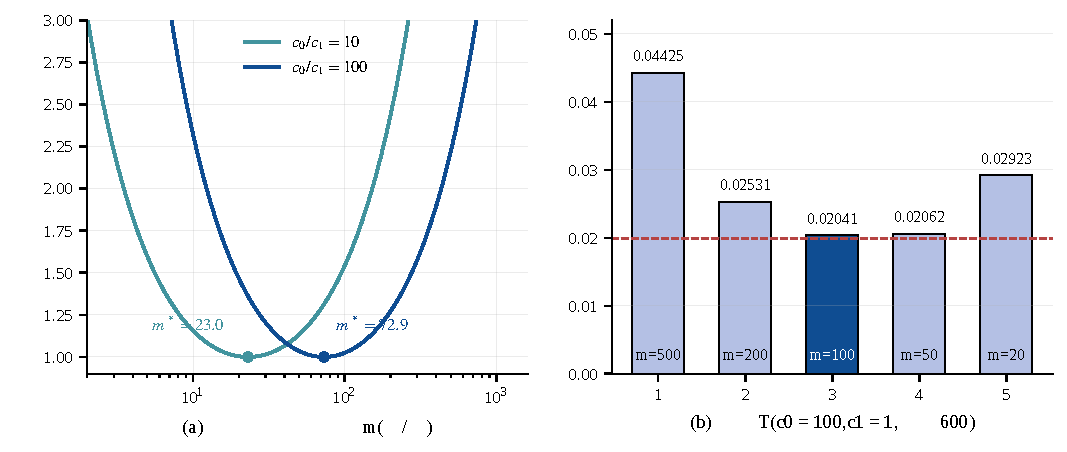
\includegraphics[width=0.95\linewidth]{figures/fig_budget.pdf}\caption{推论 1 的连续最优与整数枚举（图 1 参数）。左图横轴为单期期望报告规模 $m$（对数刻度），纵轴为目标函数 $(c_0/c_1+m)(v_R+A/m)$ 相对其最小值的倍数，$c_0/c_1=10$ 与 $100$ 两条曲线分别在 $m^*=23.0$ 与 $72.9$ 处取最小值；右图为 $c_0=100$、$c_1=1$、预算 600 时 $T=1,\dots,5$ 的跨期估计量方差，$T=3$（$m=100$）最小，红虚线为连续松弛下界。}\label{fig:pb-budget}\end{figure}

AR(1) 修正的方向与命题 4 一致。$c_0/c_1=100$、$r=0.5$ 时 $(1-r)/(1+r)=1/3$，$m^*_{\mathrm{AR}}=\sqrt{100\times53.08/3}=42.1$；$r=0.8$ 时该因子为 $1/9$，$m^*_{\mathrm{AR}}=72.86/3=24.3$。改用式~\eqref{eq:pb-exactenv} 的精确环境项、在 $\mathcal B=2\times10^4$ 下做整数搜索，最优单期规模分别为 42.9（$T=140$）与 25.0（$T=160$）。近似式高估环境项，因而略微低估最优单期规模。

\subsubsection{与仿真和实证的对应}

论文没有为推论 1 设计仿真，图 1–3 也不涉及成本。本讲义的核验覆盖了全部代数步骤：代入后的目标函数、一阶与二阶导数、唯一正根、几何平均形式、$c_0=0$ 时的单调性以及 AR(1) 替换后的 $m^*_{\mathrm{AR}}$ 均经符号核验成立；角点情形 $c_0=100$、$c_1=1$、$\mathcal B=140$ 时内部解 72.9 超过上界 40，最优取 $m^*=40$、$T=1$，与原文第 279 行一致。数值方面，第 283 行的两个区间可由第 515 行情景的 $m_\times$ 区间完全复现；图 1 参数下的 23.0 与 72.9、表~\ref{tab:pb-enum} 的整数枚举以及 AR(1) 下的 42.9 与 25.0 均为直接计算结果。实证部分估计的经验交叉点 $m_\times^{\rm emp}=22.6$ 若代入原文式 18，可得 $c_0/c_1=10$ 时的 $m^*$ 参照，但第~\ref{sec:empirical} 节指出经验 $a$、$b$ 都被放大，这一代入只能作为数量级参考。

\subsubsection{原文表述的问题}

\begin{itemize}
\item 第 283 行的数值区间紧接图 1 参数的上下文，却用了第 515 行情景的 $m_\times$，来源没有写明；建议改写为“以第 515 行流感情景的 $m_\times\in[21.3,49.2]$ 为例”，并同步修正第 515 行的 49.3。中期报告把该区间写成“14.6～24.4”，材料中不存在 24.4，属误引。
\item 推论按连续 $T$ 求解，小预算下整数最优可以与连续解相差 37\%；建议补一句“$T$ 须为整数，预算较小时应枚举”。
\item 第 283 行只说与两阶段抽样同构，建议给出表~\ref{tab:pb-cochran} 那样的符号对应与 Cochran 的章节号，答辩时可以直接引用。
\item 第 280 行的 $m^*_{\mathrm{AR}}$ 继承了原文式 16 的高估方向，与精确整数搜索相差约 2\%–3\%，建议注明近似方向，或直接用精确闭式搜索。
\end{itemize}

\subsection{命题 5：仅报告可见时的单步预测方差}

\subsubsection{原式与参数含义}

命题 5 处理时间序列情形：真实感染历史不可见，预测只能依据截至第 $t$ 期的报告历史 $\mathcal F_t^C$。原文先用更新过程描述下一期的感染压力，如下式所示：
\begin{equation*}
\Lambda_{t+1} = \sum_{s=1}^S w_s I_{t+1-s}, \qquad \sum_{s=1}^S w_s = 1.
\tag{原文式 19}
\end{equation*}
原文随后假定给定感染压力与当期传播参数时，下一期真实感染的条件均值为二者之积，如下式所示：
\begin{equation*}
\mathbb{E}[I_{t+1} \mid \Lambda_{t+1}, R_{t+1}, \mathcal{F}_t^C] = \Lambda_{t+1} R_{t+1}.
\tag{原文式 20}
\end{equation*}
报告环节沿用二项抽稀，并假定给定 $I_{t+1}$ 后报告与既往报告历史条件独立，原文第 297 行的写法如下：
\begin{equation*}
C_{t+1} \mid I_{t+1} \sim \operatorname{Binomial}(I_{t+1}, \rho)
\tag*{原文第 297 行}
\end{equation*}
命题 5（原文第 299–308 行）的第一式给出真实感染的预测方差分解：
\begin{equation*}
\operatorname{Var}(I_{t+1} \mid \mathcal{F}_t^C) = \operatorname{Var}\big(\Lambda_{t+1} R_{t+1} \;\big|\; \mathcal{F}_t^C\big) + \mathbb{E}\Big[\operatorname{Var}\big(I_{t+1} \;\big|\; \Lambda_{t+1}, R_{t+1}, \mathcal{F}_t^C\big) \;\Big|\; \mathcal{F}_t^C\Big].
\tag{原文式 21}
\end{equation*}
第二式给出报告病例的预测方差分解：
\begin{equation*}
\operatorname{Var}(C_{t+1} \mid \mathcal{F}_t^C) = \rho(1 - \rho)\,\mathbb{E}[I_{t+1} \mid \mathcal{F}_t^C] + \rho^2 \operatorname{Var}(I_{t+1} \mid \mathcal{F}_t^C).
\tag{原文式 22}
\end{equation*}

各式中出现的参数含义如下。
\begin{itemize}
\item $I_{t+1}$ 是第 $t+1$ 期的真实新发感染数，取非负整数，不可观测。
\item $\Lambda_{t+1}$ 是下一期的感染压力，即过去 $S$ 期真实感染按世代间隔权重 $w_s\ge0$ 的加权和；由于它由不可见的 $I$ 构成，给定 $\mathcal F_t^C$ 时它仍是随机变量。
\item $S$ 是世代间隔的最大滞后期数，$w_s$ 满足 $\sum_sw_s=1$。
\item $R_{t+1}$ 是第 $t+1$ 期的传播参数，含义同第~\ref{sec:model} 节。
\item $\mathcal F_t^C$ 是由报告序列 $C_1,\dots,C_t$ 生成的信息集，代表预测时刻能看到的全部数据。
\item $C_{t+1}$ 是第 $t+1$ 期的报告病例数，$\rho\in(0,1]$ 是报告率。
\end{itemize}

\subsubsection{逐步推导}

两式都由条件形式的全方差公式（附录引理~\ref{lem:ap-totvar}）得到，区别在于条件变量的选择。
\begin{enumerate}
\item 记更大的信息集 $\mathcal H=\sigma(\Lambda_{t+1},R_{t+1},\mathcal F_t^C)\supseteq\mathcal F_t^C$，由嵌套信息集下的全方差公式 $\operatorname{Var}(Y\mid\mathcal F)=\operatorname{Var}(\mathbb E[Y\mid\mathcal H]\mid\mathcal F)+\mathbb E[\operatorname{Var}(Y\mid\mathcal H)\mid\mathcal F]$，取 $Y=I_{t+1}$ 即得两项之和。
\item 把原文式 20 的条件均值 $\mathbb E[I_{t+1}\mid\mathcal H]=\Lambda_{t+1}R_{t+1}$ 代入第一项，即得原文式 21；第一项刻画感染压力与传播参数在报告信息下的不确定性，第二项刻画给定二者后的分支抽样噪声。
\item 第二式改以 $I_{t+1}$ 为条件，由全方差公式得到附录给出的展开：
\begin{equation*}
\operatorname{Var}(C_{t+1} \mid \mathcal{F}_t^C) = \mathbb{E}[\operatorname{Var}(C_{t+1} \mid I_{t+1}, \mathcal{F}_t^C) \mid \mathcal{F}_t^C] + \operatorname{Var}(\mathbb{E}[C_{t+1} \mid I_{t+1}, \mathcal{F}_t^C] \mid \mathcal{F}_t^C).
\tag*{原文第 769 行}
\end{equation*}
\item 由二项分布的均值 $np$ 与方差 $np(1-p)$，并利用报告与历史条件独立的假定（原文第 297 行），得 $\mathbb E[C_{t+1}\mid I_{t+1},\mathcal F_t^C]=\rho I_{t+1}$ 与 $\operatorname{Var}(C_{t+1}\mid I_{t+1},\mathcal F_t^C)=\rho(1-\rho)I_{t+1}$（原文第 771 行）。
\item 外层第一项由条件期望的线性性得 $\rho(1-\rho)\mathbb E[I_{t+1}\mid\mathcal F_t^C]$，外层第二项由方差的二次齐次性得 $\rho^2\operatorname{Var}(I_{t+1}\mid\mathcal F_t^C)$，两者相加即得原文式 22。
\end{enumerate}

上述推导除原文式 20 与二项报告外没有用到任何分布假定，所以命题 5 的两式是恒等式，本身不含可以计算的量。为了看清“单代公式不能直接外推”的具体含义，下面在两个附加假定下把它展开。第一个假定是：给定 $\mathcal F$（下文省略下标 $t$ 与 $t+1$），$I\mid\Lambda,R\sim\mathrm{NB}\big(k\Lambda,\,k/(k+R)\big)$，即 $\Lambda$ 个有效感染者各自按第~\ref{sec:model} 节的负二项分支产生后代（附录引理~\ref{lem:ap-nb}）。第二个假定是 $\Lambda$ 与 $R$ 在 $\mathcal F$ 下条件独立，$\mathbb E[R\mid\mathcal F]=\bar R$，$\operatorname{Var}(R\mid\mathcal F)=v_R$。记 $E_\Lambda$、$V_\Lambda$ 为 $\Lambda$ 的条件均值与条件方差，$\mathrm{CV}^2(\Lambda\mid\mathcal F)=V_\Lambda/E_\Lambda^2$。
\begin{enumerate}
\item 由负二项分布 $\mathrm{NB}(r,p)$ 的均值 $r(1-p)/p$ 与方差 $r(1-p)/p^2$，取 $r=k\Lambda$、$p=k/(k+R)$，有 $(1-p)/p=R/k$，所以条件均值为 $\Lambda R$（与原文式 20 相符），条件方差为 $\Lambda R(k+R)/k=\Lambda R+\Lambda R^2/k$。
\item 由独立随机变量乘积的二阶矩 $\mathbb E[\Lambda^2R^2]=\mathbb E[\Lambda^2]\mathbb E[R^2]$ 与 $\mathbb E[Y^2]=\operatorname{Var}(Y)+(\mathbb EY)^2$，原文式 21 的第一项为
\begin{equation*}
\operatorname{Var}(\Lambda R\mid\mathcal F)=(V_\Lambda+E_\Lambda^2)(v_R+\bar R^2)-E_\Lambda^2\bar R^2=V_\Lambda v_R+V_\Lambda\bar R^2+E_\Lambda^2v_R .
\end{equation*}
\item 由条件独立下期望的乘积性质，原文式 21 的第二项为 $\mathbb E[\Lambda R+\Lambda R^2/k\mid\mathcal F]=E_\Lambda\bar R+E_\Lambda(\bar R^2+v_R)/k$；同理 $\mathbb E[I\mid\mathcal F]=E_\Lambda\bar R$。
\item 把第 2、3 步代入原文式 22，并用 $\rho(1-\rho)E_\Lambda\bar R+\rho^2E_\Lambda\bar R=\rho E_\Lambda\bar R$ 合并两个一次项，得
\begin{equation*}
\operatorname{Var}(C\mid\mathcal F)=\rho E_\Lambda\bar R+\frac{\rho^2E_\Lambda(\bar R^2+v_R)}{k}+\rho^2E_\Lambda^2v_R+\rho^2V_\Lambda(\bar R^2+v_R).
\end{equation*}
\item 记 $m\triangleq\rho E_\Lambda$（下一期的期望报告规模在 $R$ 取 1 时的刻度），两边除以 $m^2$；前两项分别化为 $\bar R/m$ 与 $\rho(\bar R^2+v_R)/(km)$，合起来正是 $A/m$，于是
\begin{equation}
\frac{\operatorname{Var}(C\mid\mathcal F)}{(\rho E_\Lambda)^2}=v_R+\frac{A}{m}+\mathrm{CV}^2(\Lambda\mid\mathcal F)\,(\bar R^2+v_R).\label{eq:pb-expand}
\end{equation}
\end{enumerate}
式~\eqref{eq:pb-expand} 的左端是统计量 $C/(\rho E_\Lambda)$ 的条件方差，这个统计量在感染压力已知时就是命题 2 中的单期估计量。当 $\Lambda$ 在 $\mathcal F$ 下已知时 $\mathrm{CV}^2=0$，式~\eqref{eq:pb-expand} 恰好退化为命题 2 的 $v_R+A/m$；真实感染不可见带来的额外项是 $\mathrm{CV}^2(\Lambda\mid\mathcal F)(\bar R^2+v_R)$，它不随 $m$ 以 $1/m$ 衰减，大小取决于从报告历史反推感染压力的精度。

\subsubsection{直觉与数值例}

原文式 22 的两项分别对应两层随机性：给定真实感染后报告环节的二项噪声，以及真实感染本身的预测不确定性经 $\rho^2$ 缩放后的贡献。式~\eqref{eq:pb-expand} 进一步把后者拆成三块，其中前两块与单代模型相同，第三块是“看不见感染”这一事实本身的代价。

取图 1 参数 $\bar R=1.15$、$v_R=0.04$、$k=0.35$、$\rho=0.25$（$A=2.1232$），并设 $E_\Lambda=40$，则 $m=\rho E_\Lambda=10$。
\begin{itemize}
\item 感染压力已知（$\mathrm{CV}=0$）时，式~\eqref{eq:pb-expand} 右端为 $0.04+2.1232/10=0.25232$，乘以 $m^2=100$ 得 $\operatorname{Var}(C\mid\mathcal F)=25.23$；真实感染的预测方差为 $40\times1.15+40\times1.3625/0.35+40^2\times0.04=46+155.71+64=265.71$。
\item 感染压力的条件变异系数为 $\mathrm{CV}=0.3$ 时，额外项为 $0.09\times1.3625=0.12263$，右端变为 $0.37495$，$\operatorname{Var}(C\mid\mathcal F)=37.49$，比感染压力已知时高 48.6\%；真实感染的预测方差增加 $V_\Lambda(\bar R^2+v_R)=144\times1.3625=196.2$，变为 461.9。
\item 设 $E_\Lambda=200$、$\mathrm{CV}=0.5$，则 $m=50$，右端为 $0.04+0.04246+0.25\times1.3625=0.42309$，$\operatorname{Var}(C\mid\mathcal F)=0.42309\times2500=1057.72$。此时额外项 0.3406 远大于规模项 0.0425，继续扩大单期规模几乎无法降低预测方差。
\end{itemize}

\subsubsection{与仿真和实证的对应}

蒙特卡洛核验在上述三种配置下检验了原文式 21、式 22 与式~\eqref{eq:pb-expand}。真实感染方差的模拟值 266.1、456.6、16065.4 与理论值 265.7、461.9、16233.6 的偏离都在 $|z|<3$ 内；报告病例方差在 $\mathrm{CV}=0$ 时模拟值 25.24 对理论 25.23，$E_\Lambda=200$、$\mathrm{CV}=0.5$ 时 1048.12 对 1057.72（$z=-1.76$）。$E_\Lambda=40$、$\mathrm{CV}=0.3$ 的报告病例方差单次模拟为 36.97，对理论 37.49 的 $z=-4.45$；用 20 组独立随机数流各 $10^4$ 次重复复核后，相对误差为 $-0.07\%\pm0.27\%$，与零无差异，所以这是重尾分布下单次模拟的波动，与公式无关。感染压力固定时，$\operatorname{Var}(C)/(\rho\Lambda)^2$ 的模拟值 0.2524 与命题 2 的 0.2523 一致，验证了退化关系。

论文本身没有为命题 5 单独设计仿真。式~\eqref{eq:pb-expand} 的额外项为图 3 的更新过程仿真提供了解释框架：在更新过程中感染压力由报告历史近似，额外项不随规模衰减，这与本节后文式 28 中的偏差项方向一致。第~\ref{sec:empirical} 节实证截距 $a$ 高于情景隐含 $v_R/\bar R^2$ 的现象，也需要这类额外项参与解释。

\subsubsection{原文表述的问题}

\begin{itemize}
\item 命题 5 的两式是对任意分布都成立的全方差恒等式，命题本身没有用到负二项结构，也没有给出可计算的结论。第 309 行称它表明“单代静态公式不能直接外推”，但这一含义要在式~\eqref{eq:pb-expand} 的展开中才看得见；建议把该展开作为命题 5 的推论写进正文。
\item 第 312 行“瓶颈属于目标 B；作为对照，目标 A 在单期不存在瓶颈……”与上下文没有衔接，其中的“目标 A”又与方差系数 $A$ 同名；建议删除，或改写为式~\eqref{eq:pb-expand} 额外项的解释。
\item 附录第 756 行标题“命题 5 的数学证明”实际证明的是正文命题 6（增长检验），第 761 行标题“命题 6 的数学证明”实际证明的是正文命题 5（预测方差分解）。正文第 310、336 行的交叉引用指向正确的 label，错误只在标题文字；建议交换两个小节的标题，答辩材料一律按正文编号。
\end{itemize}

\subsection{命题 6：精确增长检验与功效}

\subsubsection{原式与参数含义}

命题 6 利用命题 1 的精确负二项条件分布，检验当期传播是否超临界。原文的单侧假设如下式所示：
\begin{equation*}
H_0: R_t \le 1 \qquad \text{对} \qquad H_1: R_t > 1.
\tag{原文式 23}
\end{equation*}
命题 6(i) 规定离散临界值取使边界点超额拒绝概率受控的最小整数：
\begin{equation*}
c_\alpha = \min \left\{ c \in \mathbb{N} \;:\; \Pr_{R_t = 1}(C_t \ge c) \le \alpha \right\};
\tag{原文式 24}
\end{equation*}
命题 6(ii) 给出备择 $R_t=1+\delta$ 下的精确功效：
\begin{equation*}
\pi(n, \delta) \triangleq \Pr_{R_t = 1 + \delta}(C_t \ge c_\alpha) = 1 - F_{\operatorname{NB}}\!\left(c_\alpha - 1; \; nk, \; \frac{k}{k + \rho(1+\delta)}\right),
\tag{原文式 25}
\end{equation*}
其中负二项累积分布函数的参数化由原文第 332 行给出：
\begin{equation*}
F_{\operatorname{NB}}(x; r, p) = \sum_{j=0}^{\lfloor x \rfloor} \frac{\Gamma(j+r)}{j!\Gamma(r)} p^r (1-p)^j
\tag*{原文第 332 行}
\end{equation*}
附录证明单调似然比时使用的概率质量函数（省略了与 $R_t$ 无关的因子）如下：
\begin{equation*}
\Pr(C_t = j) \propto (k/(k+\rho R_t))^{nk}(1-p^*)^j
\tag*{原文第 758 行}
\end{equation*}
第 4.1 节作为对照的 Wald 检验统计量如下：
\begin{equation*}
Z = (\widehat{R}_t - 1)/\sqrt{V_0}
\tag*{原文第 350 行}
\end{equation*}
其零假设方差如下：
\begin{equation*}
V_0 = \frac{1}{\rho n} + \frac{1}{kn}
\tag*{原文第 350 行}
\end{equation*}

各式中出现的参数含义如下。
\begin{itemize}
\item $n$ 是上一代感染者数（真实风险集规模），$k>0$ 是个体离散参数，$\rho\in(0,1]$ 是报告率；命题 6 假定三者已知。
\item $R_t>0$ 是当期传播参数，$R_t=1$ 是亚临界与超临界的分界。
\item $C_t$ 是当期报告病例数，在给定 $(n,\rho,k)$ 时它是 $R_t$ 的充分统计量。
\item $\alpha\in(0,1)$ 是名义检验水平，论文取 $0.05$；$c_\alpha\in\mathbb N$ 是离散临界值。
\item $\delta>0$ 是备择增长强度，$\pi(n,\delta)$ 是精确功效。
\item $p^*=k/(k+\rho R_t)$ 是抽稀后负二项分布的成功概率；$F_{\operatorname{NB}}(x;r,p)$ 中的 $r$ 是形状参数，此处取 $r=nk$，与命题 4 的 AR(1) 系数无关。
\item $z_{1-\alpha}$ 是标准正态分布的 $1-\alpha$ 分位数，Wald 检验在 $Z\ge z_{1-\alpha}$ 时拒绝 $H_0$。
\end{itemize}

\subsubsection{逐步推导}

由命题 1 与附录引理~\ref{lem:ap-thin}，$C_t\mid n,R_t\sim\mathrm{NB}(nk,p^*)$，概率质量函数为 $\frac{\Gamma(j+nk)}{j!\Gamma(nk)}(p^*)^{nk}(1-p^*)^j$，其中 $1-p^*=\rho R_t/(k+\rho R_t)$。推导分九步。
\begin{enumerate}
\item 对任意 $R'>R$ 作似然比，组合因子 $\Gamma(j+nk)/(j!\Gamma(nk))$ 与 $R$ 无关而相消，似然比如下：
\begin{equation}
\frac{\Pr_{R'}(C_t=j)}{\Pr_{R}(C_t=j)}=\Big(\frac{p^*(R')}{p^*(R)}\Big)^{nk}\Big(\frac{1-p^*(R')}{1-p^*(R)}\Big)^{j},\label{eq:pb-lr}
\end{equation}
这个比值的对数关于 $j$ 是线性函数，斜率为 $\ln[(1-p^*(R'))/(1-p^*(R))]$。
\item 由商的求导法则，$\frac{\mathrm d}{\mathrm dR}\frac{\rho R}{k+\rho R}=\frac{\rho(k+\rho R)-\rho^2R}{(k+\rho R)^2}=\frac{\rho k}{(k+\rho R)^2}>0$，所以 $1-p^*$ 关于 $R$ 严格递增，式~\eqref{eq:pb-lr} 的斜率为正，似然比关于 $j$ 严格递增，负二项族关于 $C_t$ 具有单调似然比性质。
\item 由单调似然比蕴含一阶随机占优的标准结论 \citep{lehmann2005testing}，对任意整数 $c$，尾概率 $\Pr_R(C_t\ge c)$ 关于 $R$ 单调不减；因此 $\sup_{R\le1}\Pr_R(C_t\ge c)=\Pr_{1}(C_t\ge c)$，复合原假设下的水平只需在边界 $R_t=1$ 处校准。
\item 记 $g(c)=\Pr_1(C_t\ge c)$，它关于 $c$ 单调不增，$g(0)=1>\alpha$，且由于 $C_t$ 的分布是正常的概率分布，$g(c)\to0$；所以集合 $\{c\in\mathbb N:g(c)\le\alpha\}$ 非空，由自然数的良序性其最小元 $c_\alpha$ 存在，并且最小性给出 $g(c_\alpha-1)>\alpha$。
\item 检验 $\{C_t\ge c_\alpha\}$ 的实际水平为 $\alpha^*=g(c_\alpha)\le\alpha$；$g$ 只取可数多个值，等号仅在 $\alpha$ 恰好等于其中某个值时成立，所以一般陈述只能写“不超过 $\alpha$”。
\item 由 Karlin–Rubin 定理 \citep{karlin1956theory,lehmann2005testing}，对具有单调似然比的分布族，随机化检验 $\phi=\mathbb 1\{C_t>c_\alpha-1\}+\gamma\,\mathbb 1\{C_t=c_\alpha-1\}$ 在 $\gamma=(\alpha-g(c_\alpha))/(g(c_\alpha-1)-g(c_\alpha))\in[0,1)$ 时边界水平恰为 $\alpha$，是检验 $H_0:R_t\le1$ 对 $H_1:R_t>1$ 的水平 $\alpha$ 一致最大功效检验；非随机化检验对应 $\gamma=0$，它只在自身的实际水平 $\alpha^*$ 下是一致最大功效检验，在水平 $\alpha$ 的检验类中功效低于随机化检验。
\item 在备择 $R_t=1+\delta$ 下，由补事件公式 $\Pr(C_t\ge c)=1-\Pr(C_t\le c-1)$，并把 $p^*$ 中的 $R_t$ 换成 $1+\delta$，即得原文式 25。
\item 由负二项分布的可加性，$\mathrm{NB}(nk,p^*)$ 是 $n$ 个独立 $\mathrm{NB}(k,p^*)$ 之和，所以 $C_t$ 关于 $n$ 随机递增，$c_\alpha(n)$ 关于 $n$ 单调不减（附录第 758 行的注记）；但 $n\to n+1$ 时零假设与备择下的分布同时右移，若 $c_\alpha$ 不变则水平与功效同时上升，若 $c_\alpha$ 跳升则二者同时下降，所以 $\pi(n,\delta)$ 关于 $n$ 呈锯齿状且非单调，满足功效要求的最小样本量必须逐点枚举。
\item 对 Wald 检验，由命题 1 的条件方差在 $R_t=1$ 处取值得 $V_0=1/(\rho n)+1/(kn)$；由于 $\widehat R_t=C_t/(\rho n)$ 且 $C_t$ 取整数，拒绝域 $\{Z\ge z_{1-\alpha}\}$ 等价于 $\{C_t\ge\lceil\rho n(1+z_{1-\alpha}\sqrt{V_0})\rceil\}$，所以 Wald 检验的精确水平可以直接由负二项尾概率算出：
\begin{equation}
\alpha_{\rm Wald}=1-F_{\operatorname{NB}}\big(\lceil\rho n(1+z_{1-\alpha}\sqrt{V_0})\rceil-1;\ nk,\ k/(k+\rho)\big).\label{eq:pb-wald}
\end{equation}
\end{enumerate}

\subsubsection{直觉与数值例}

$C_t$ 越大越支持 $R_t>1$，单调似然比保证了“报告数超过阈值即报警”这一直觉做法在已知 $(n,\rho,k)$ 时是最优形状的检验。离散性带来两个代价：实际水平一般低于 $\alpha$，功效随 $n$ 锯齿上升。

取 $k=0.35$、$\rho=0.25$、$\alpha=0.05$。$n=100$ 时直接计算得 $c_\alpha=37$，实际水平 0.0488。再取 $\delta=0.30$ 观察锯齿：$n=568$ 时 $c_\alpha=169$，实际水平 0.0490，功效 0.8015，首次达到 0.8；$n=569$ 时 $c_\alpha$ 跳到 170，实际水平降为 0.0448，功效跌回 0.7907。图~\ref{fig:pb-power} 画出 $n=450$ 到 699 的全貌：左图功效在整体上升的趋势上叠加锯齿，在 $n=400$ 到 699 范围内共有 82 处下降；右图实际水平在 0.05 以下锯齿波动，每次临界值跳升都对应一次骤降。

\begin{figure}[!tbp]\centering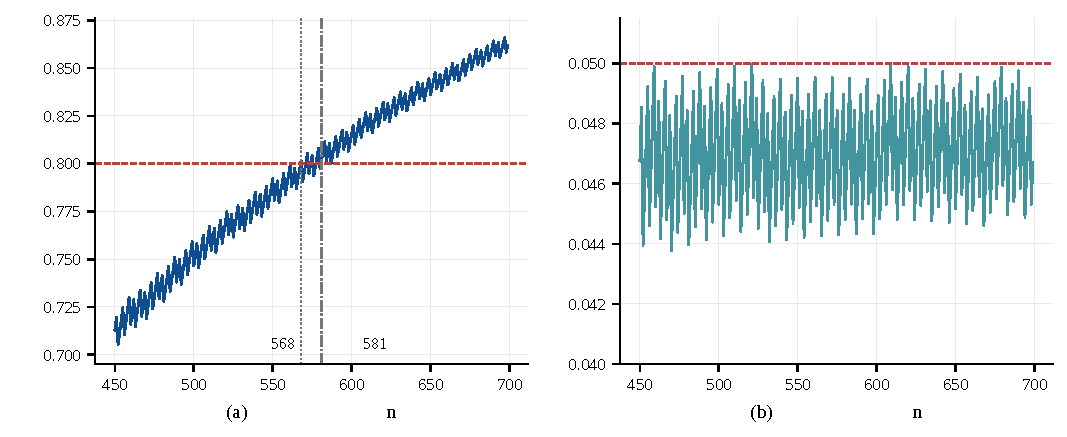
\includegraphics[width=0.95\linewidth]{figures/fig_power_sawtooth.pdf}\caption{精确增长检验的功效与实际水平随上一代感染者数 $n$ 的锯齿变化（$k=0.35$，$\delta=0.30$，$\rho=0.25$，$\alpha=0.05$）。左图为精确功效，红虚线为 0.8，两条竖线分别标出首次达到 0.8 的 $n=568$ 与此后稳定不低于 0.8 的 $n=581$；右图为实际检验水平，始终不超过 0.05 并随临界值跳升锯齿波动。}\label{fig:pb-power}\end{figure}

由于功效非单调，“首次达到 0.8 的 $n$”与“此后恒不低于 0.8 的 $n$”是两个不同的量。表~\ref{tab:pb-power} 列出论文图 2 的五组配置，稳定样本量比首次样本量多 1.4\%–3.0\%。

\begin{table}[!tbp]\centering\small\caption{论文图 2 五组配置下首次与稳定达到 80\% 功效的样本量（$\rho=0.25$，$\alpha=0.05$）}\label{tab:pb-power}
\begin{tabular}{L{1.6cm}L{1.6cm}L{2.4cm}L{2.4cm}L{2.0cm}L{3.2cm}}
\toprule
$k$ & $\delta$ & 首次 $n$（$m=\rho n$） & 稳定 $n$（$m=\rho n$） & 增幅 & 首次之后跌回 0.8 以下的 $n$ 个数 \\
\midrule
0.35 & 0.15 & 2071（517.75） & 2107（526.75） & 1.7\% & 19 \\
0.35 & 0.30 & 568（142.00） & 581（145.25） & 2.3\% & 7 \\
0.35 & 0.50 & 229（57.25） & 235（58.75） & 2.6\% & 2 \\
1.0 & 0.25 & 568（142.00） & 585（146.25） & 3.0\% & 9 \\
0.1 & 0.25 & 1660（415.00） & 1684（421.00） & 1.4\% & 10 \\
\bottomrule
\end{tabular}
\end{table}

Wald 检验的精确水平可以按式~\eqref{eq:pb-wald} 手算。取 $m=5$（$n=20$）、$k=0.1$：$V_0=1/5+1/2=0.7$，$\sqrt{V_0}=0.8367$，$z_{0.95}=1.6449$，阈值 $5\times(1+1.6449\times0.8367)=11.88$，取整为 12；$C_t\sim\mathrm{NB}(2,\,0.1/0.35)$ 时 $\Pr(C_t\ge12)=0.0781$，高于名义水平 0.05。

\subsubsection{与仿真和实证的对应}

论文图 2（原文第 353–359 行）检验的就是命题 6。核验结果如下。
\begin{itemize}
\item 符号核验确认式~\eqref{eq:pb-lr} 的对数斜率与 $1-p^*$ 的导数；在 200 组随机 $(n,k,R<R')$ 下，似然比在 $j=0,\dots,499$ 上严格递增，没有违例。$n=100$、$k=0.35$ 时尾概率在 $R\in[0.3,1]$ 上单调，最大值 0.0488 在 $R=1$ 处取得。
\item 在 $k\in\{0.1,0.35,1\}$、$n\le3000$ 的网格上，精确检验的实际水平最大 0.05000、最小 0.01696，没有恰好等于 0.05 的点；$c_\alpha(n)$ 关于 $n$ 单调不减。
\item 图 2(b)(c) 报告的五个“首次达到 80\% 功效”的 $n$（2071/568/229/568/1660）全部被精确复现；图 2(c) 所说“近 3 倍”的样本需求放大实为 2.92 倍。
\item 图 2(a) 的 Wald 检验经验水平可以由式~\eqref{eq:pb-wald} 精确计算：$m=5$、$k=0.1$ 时精确值 0.0781，论文 30000 次模拟的 0.081 落在模拟误差 $\pm2\sigma$（$\pm0.0031$）带内，$2\times10^5$ 次复核得 0.0789；$k=1$ 时精确值 0.0493 与 0.0691，与论文的 0.0495 与 0.0691 一致。在 $k\le0.35$、$m<40$ 的 14 个网格点上精确水平全部高于 0.05，论文“系统性过检”的结论成立。
\end{itemize}

\subsubsection{原文表述的问题}

\begin{itemize}
\item 第 340 行称非随机化检验的实际水平“严格低于名义水平 $\alpha$”，一般陈述中应改为“不超过 $\alpha$”；第 323 行“严格控制在 $\alpha$ 以内”的表述可以保留。
\item 正文若使用“最优”一词，应写明非随机化检验只在它的实际水平下一致最优；若需要恰好水平 $\alpha$，可改用第 6 步的随机化检验。
\item 以上结论都在 $k$ 已知时成立；实际应用中以估计值 $\hat k$ 代入时水平不再有精确保证，论文的局限性部分应补充这一点。
\item 图 2 只报告首次达到 80\% 功效的 $n$，建议同时报告表~\ref{tab:pb-power} 的稳定样本量；第 364 行的 Wald 水平建议改报式~\eqref{eq:pb-wald} 的精确值。
\end{itemize}

\subsection{更新过程仿真中的恒等式}

\subsubsection{原式与参数含义}

论文在时间序列更新过程中评价两类误差，所用的恒等式与分解是命题 5 在仿真中的落地形式。预测时刻已知的历史报告加权和定义如下：
\begin{equation*}
D_t \triangleq \sum_{s=1}^S w_s C_{t+1-s}.
\tag{原文式 26}
\end{equation*}
事后代理增长统计量由原文第 379 行定义如下：
\begin{equation*}
G_{t+1} \triangleq C_{t+1}/D_t
\tag*{原文第 379 行}
\end{equation*}
事前单步预测由原文第 380 行定义如下：
\begin{equation*}
\widehat{C}_{t+1 \mid t} \triangleq \bar{R} D_t
\tag*{原文第 380 行}
\end{equation*}
两者的误差由下面的恒等式联系起来：
\begin{equation*}
\operatorname{RelMSE}(m) \triangleq \mathbb{E}\left[\left(\frac{C_{t+1} - \widehat{C}_{t+1 \mid t}}{\widehat{C}_{t+1 \mid t}}\right)^2 \;\middle|\; D_t > 0\right] = \frac{1}{\bar{R}^2}\mathbb{E}\left[(G_{t+1} - \bar{R})^2 \;\middle|\; D_t > 0\right].
\tag{原文式 27}
\end{equation*}
条件预测矩由原文第 387 行定义如下：
\begin{equation*}
\mu_{t+1 \mid t} \triangleq \mathbb{E}[C_{t+1} \mid \mathcal{F}_t^C]
\tag*{原文第 387 行}
\end{equation*}
\begin{equation*}
\sigma_{t+1 \mid t}^2 \triangleq \operatorname{Var}(C_{t+1} \mid \mathcal{F}_t^C)
\tag*{原文第 387 行}
\end{equation*}
活跃周上的条件分解如下：
\begin{equation*}
\mathbb{E}\left[(G_{t+1} - \bar{R})^2 \;\middle|\; D_t > 0\right] = \mathbb{E}\left[\frac{\sigma_{t+1 \mid t}^2}{D_t^2} + \left(\frac{\mu_{t+1 \mid t}}{D_t} - \bar{R}\right)^2 \;\middle|\; D_t > 0\right].
\tag{原文式 28}
\end{equation*}
参照曲线 $V(m)=v_R+A/m$ 在规模翻倍时的相对降幅如下：
\begin{equation*}
\frac{V(m) - V(2m)}{V(m)} = \frac{1}{2(1 + m/m_\times)}.
\tag{原文式 29}
\end{equation*}

各式中出现的参数含义如下。
\begin{itemize}
\item $D_t\ge0$ 是用报告病例按世代间隔权重 $w_s$ 加权得到的历史规模，它关于 $\mathcal F_t^C$ 可测；给定真实感染历史时 $\mathbb E[D_t\mid I]=\rho\Lambda_{t+1}$，所以 $D_t$ 是感染压力的一个带二项噪声的代理。
\item $G_{t+1}$ 是事后代理增长统计量，只在 $D_t>0$ 的活跃周有定义。
\item $\widehat C_{t+1\mid t}$ 是以已知基础水平 $\bar R$ 乘历史规模得到的事前预测；$\operatorname{RelMSE}(m)$ 是活跃周上的相对均方预测误差，$m$ 是每条仿真轨迹的初始期望报告规模。
\item $\mu_{t+1\mid t}$ 与 $\sigma^2_{t+1\mid t}$ 是给定报告历史时下一期报告数的条件均值与条件方差，后者就是命题 5 中原文式 22 的左端。
\item $V(m)=v_R+A/m$ 是命题 2 的单代参照曲线，$m_\times=A/v_R$ 是交叉点；仿真取图 1 参数，$m_\times=53.08$，$\bar R=1.15$，$\bar R^2=1.3225$。
\end{itemize}

\subsubsection{逐步推导}

原文式 27 只用到代数恒等变形，推导分三步。
\begin{enumerate}
\item 在 $D_t>0$ 的事件上代入 $\widehat C_{t+1\mid t}=\bar RD_t$，分子分母同除以 $D_t$，得 $(C_{t+1}-\bar RD_t)/(\bar RD_t)=(G_{t+1}-\bar R)/\bar R$。
\item 两边平方，得到逐观测成立的等式，左端是相对预测误差的平方，右端是 $(G_{t+1}-\bar R)^2/\bar R^2$。
\item 由条件期望的线性性，在同一事件 $\{D_t>0\}$ 上取条件期望，并把常数 $1/\bar R^2$ 提到期望外，即得原文式 27。由于等式逐观测成立，它对同一活跃周子集上的样本平均同样成立，两类误差的翻倍降幅中常数 $1/\bar R^2$ 相消，所以两者的经验降幅完全相同。
\end{enumerate}

原文式 28 的推导要用到“提出已知量”与塔式性质，分五步。
\begin{enumerate}
\item 以 $\mu=\mu_{t+1\mid t}$ 为中心作加减拆分，得 $G_{t+1}-\bar R=(C_{t+1}-\mu)/D_t+(\mu/D_t-\bar R)$。第一项是围绕条件均值的波动，第二项是用报告历史代理感染压力造成的偏差。
\item 由完全平方公式展开，平方项分成波动平方 $(C_{t+1}-\mu)^2/D_t^2$、交叉项 $2(C_{t+1}-\mu)(\mu/D_t-\bar R)/D_t$ 与偏差平方 $(\mu/D_t-\bar R)^2$ 三部分。
\item 由于 $D_t$ 由 $C_t,\dots,C_{t+1-S}$ 构成，它关于 $\mathcal F_t^C$ 可测，$\mu$ 也关于 $\mathcal F_t^C$ 可测。由条件期望“提出已知量”的性质，波动平方的条件期望为 $\sigma^2_{t+1\mid t}/D_t^2$，偏差平方原样保留，交叉项的条件期望含因子 $\mathbb E[C_{t+1}-\mu\mid\mathcal F_t^C]=0$，因而为零。
\item 于是在 $\{D_t>0\}$ 上有 $\mathbb E[(G_{t+1}-\bar R)^2\mid\mathcal F_t^C]=\sigma^2_{t+1\mid t}/D_t^2+(\mu_{t+1\mid t}/D_t-\bar R)^2$。
\item 事件 $\{D_t>0\}$ 属于 $\mathcal F_t^C$，由塔式性质，对第 4 步两端再取以该事件为条件的期望，即得原文式 28。
\end{enumerate}

原文式 29 的推导分三步。
\begin{enumerate}
\item 由 $V(m)=v_R+A/m$，环境项在差分中相消，分子为 $V(m)-V(2m)=A/m-A/(2m)=A/(2m)$。
\item 除以 $V(m)$ 并把分子分母同乘 $m$，得 $A/[2(v_Rm+A)]$。
\item 分子分母同除以 $A$，并代入 $m_\times=A/v_R$，即得原文式 29。这个降幅等于规模项在总方差中所占份额的一半，上限 50\% 只在 $m\to0$ 时取到。
\end{enumerate}

最后说明原文式 28 推不出“经验误差始终不低于单代下界”，理由分三步。
\begin{enumerate}
\item 原文式 28 中偏差项非负，由期望的单调性只能得到 $\mathbb E[(G_{t+1}-\bar R)^2\mid D_t>0]\ge\mathbb E[\sigma^2_{t+1\mid t}/D_t^2\mid D_t>0]$。
\item 若要进一步得到不低于 $v_R+A/m$，还需要右端不低于 $v_R+A/m$。式~\eqref{eq:pb-expand} 给出的是 $\sigma^2_{t+1\mid t}$ 除以 $(\rho E_\Lambda)^2$ 后的展开，原文式 28 除的却是报告历史 $D_t^2$；$D_t/(\rho E_\Lambda)$ 是随机比值，增长期的 $\mu/D_t$ 也会偏离 $\bar R$，所以两者的大小关系方向不定。
\item 参照曲线中的 $m$ 是初始规模，增长期评价周的实际规模远大于初始值，横轴口径不同也会改变比较结果。因此“始终不低于单代下界”只能作为特定口径下的经验观察，没有定理的地位。
\end{enumerate}

\subsubsection{直觉与数值例}

原文式 27 说明事前预测误差与事后增长统计量误差是同一个量的两种写法。原文式 28 把它拆成两块：随机分母使条件方差按 $1/D_t^2$ 重新加权，偏差项则反映用报告历史代替真实感染压力的系统误差。

翻倍降幅按原文式 29 计算，图 1 参数下 $m_\times=53.08$。$m=10$ 时降幅为 42.1\%，$m=m_\times$ 时为 25.0\%，$m=200$ 时为 10.5\%，首点 $m=6$ 时为 44.9\%。

小规模端的数值都可以由参照曲线逐项复算，表~\ref{tab:pb-small} 汇总了 $m=6$ 与 $m=12$ 两组的计算过程。$m=6$ 时经验相对误差是参照值的 1.82 倍；$m=12$ 时经验值 0.190 已低于参照值 0.217；首点 $m=6\to12$ 的经验翻倍降幅 73.5\% 远高于原文式 29 给出的 44.9\%。

\begin{table}[!tbp]\centering\small\caption{更新过程仿真小规模端数值的复算（图 1 参数）}\label{tab:pb-small}
\begin{tabular}{L{4.6cm}L{5.4cm}L{2.4cm}}
\toprule
量 & 计算 & 结果 \\
\midrule
$m=6$ 参照值 $v_R+A/6$ & $0.04+2.12321/6$ & 0.394 \\
$m=6$ 参照相对误差 & $0.39387/1.3225$ & 0.298 \\
$m=6$ 经验相对误差 & 论文报告值 & 0.543 \\
$m=6$ 经验与参照之比 & $0.543/0.298$ & 1.82 \\
$m=12$ 参照值 $v_R+A/12$ & $0.04+2.12321/12$ & 0.217 \\
$m=12$ 经验值 & 论文报告值 & 0.190 \\
环境底板 $v_R/\bar R^2$ & $0.04/1.3225$ & 0.0302 \\
首点经验翻倍降幅 & $(0.543\times1.3225-0.190)/(0.543\times1.3225)$ & 73.5\% \\
\bottomrule
\end{tabular}
\end{table}

\subsubsection{与仿真和实证的对应}

这一组恒等式对应论文图 3 以及第 393、399、405、406、409 行的文字，核验结果如下。
\begin{itemize}
\item 原文式 27 的逐观测恒等与原文式 28 的条件分解经符号核验成立；在 $m=6$ 到 200 的各规模组上，分解两端的蒙特卡洛估计彼此一致。
\item 表~\ref{tab:pb-small} 的全部数值以及论文报告的剔除率（$m=6$ 组 0.077\%，$m=12$ 组 0.026\%）均被复现；翻倍降幅 42.1\%、25.0\%、10.5\% 与原文式 29 的代入结果一致。
\item 第 393 行的横轴口径数值可以复现到相近范围。按初始 $m$，$m\ge25$ 段经验与参照之比在论文中为 0.75–0.98，本讲义重算为 0.77–0.92；按实现规模分箱，论文为 1.01–1.17，重算为 1.03–1.12；评价周实际规模中位数与初始 $m$ 之比，论文为 1.7–2.4 倍，重算为 1.82–2.36 倍。
\end{itemize}
按初始规模的比值低于 1，说明参照曲线在这一口径下高于经验误差；只有按实现规模分箱时比值才高于 1。第~\ref{sec:empirical} 节的实证分母同样由报告病例构造，随机分母对斜率的放大与这里 $1/D_t^2$ 的重新加权属于同一机制。

\subsubsection{原文表述的问题}

\begin{itemize}
\item 第 393 行与第 406 行称更新过程经验误差“始终不低于单代静态下界”，并把它与原文式 28 联系起来。由上文推导的最后三步，原文式 28 只保证偏差项非负，推不出不低于 $v_R+A/m$；按初始规模的比值 0.75–0.98 本身就低于 1。建议改为“按实现规模分箱时，本仿真中经验误差不低于参照曲线（1.01–1.17 倍），方向与非负偏差项一致，但这不构成一般性下界”。
\item 第 375 行的 $\max(1,I)$ 截断改变了小规模端的数据生成过程，论文说明了偏差方向，但没有报告各规模组的触发频率，建议补充，尤其是 $m=6$ 组。
\item 首点经验降幅 73.5\% 高于解析值 44.9\%，正文可以补一句原因：小规模端的偏差项与随机分母的贡献随规模迅速衰减，降幅因此叠加了参照曲线之外的部分。
\end{itemize}


\section{从理论到实证}\label{sec:empirical}
本章把第~\ref{sec:props} 节的理论结论放到原文实证节（第 424--650 行）中逐项对照。理论刻画的是“风险集已知、一代传播、报告率已知”条件下估计量的方差结构。实证使用的是由报告病例构造的周度增长代理，两者之间隔着若干步近似。本章先说明数据和变量的构造，再确定理想条件下仿射模型参数对应的理论量，并解释实际估计值偏离这些理论量的原因。随后讨论 FGLS、聚类 Bootstrap 与工具变量成立的条件，最后逐张解读原文的实证表。每一处偏离都给出定量依据，并标注第~\ref{sec:checks} 节问题表中的编号（I-xx）。

\subsection{数据构造与仿射模型}

原文使用全美各州及华盛顿特区医院向 CDC NHSN 上报的周度实验室确诊流感住院人数与各州医院报告覆盖率 \citep{cdc2026nhsn}。该住院指标自 2021--22 赛季起是 CDC FluSight 的核心预测目标 \citep{mathis2024evaluation}。样本覆盖 2020 年 8 月至 2026 年 9 月、50 个州及华盛顿特区，共 16,218 个州–周观测。其中 504 个州–周的住院数缺失，原文按 0 例处理（第一阶段 468 个、第二阶段 36 个）。制度切换期的“未填报”与“零住院”含义不同，原文第 430 行已把这一处理的影响限定在第二阶段。

样本筛选只有一条规则：历史有效输入压力 $D_t\ge5$ 的州–周进入推断样本，共 10,303 个；原文不另设覆盖率门槛，以免系统性剔除低覆盖观测。这 10,303 个观测按报告制度分为三个阶段，见表~\ref{tab:em-phase}。第二阶段覆盖率从 91.1\% 跌到 54.6\%，原文把它当作报告率杠杆 $\rho$ 的制度层面代理，第~\ref{sec:em-space} 小节检验这一代理能解释多少观测噪声的变化。

\begin{table}[!tbp]
\centering
\small
\caption{原文三个报告制度阶段的划分与覆盖率（依据原文第 430--437 行）}
\label{tab:em-phase}
\begin{tabular}{L{2.6cm}L{4.4cm}L{1.1cm}L{1.3cm}L{1.9cm}L{1.7cm}}
\toprule
阶段 & 时间范围 & 有效周 & 样本数 $N$ & 覆盖率（样本平均） & 覆盖率中位数 \\
\midrule
前过渡高覆盖期 & 2020 年 10 月至 2024 年 4 月 30 日 & 184 & 6,009 & 91.1\% & 92.3\% \\
自愿过渡期 & 2024 年 5 月 1 日至 2024 年 10 月 31 日 & 26 & 420 & 54.6\% & 45.7\% \\
CMS 新规重制期 & 2024 年 11 月 1 日至 2026 年 9 月初 & 96 & 3,874 & 91.8\% & 93.2\% \\
\bottomrule
\end{tabular}
\par\smallskip
\begin{minipage}{0.92\linewidth}\footnotesize
注：样本数为 $D_t\ge5$ 筛选后的州–周数，三阶段合计 10,303。第一阶段合并了大流行早期段（$N=2{,}627$，覆盖率 87.8\%）与 2022 年 10 月起的法定强制段（$N=3{,}382$，覆盖率 93.7\%）。
\end{minipage}
\end{table}

原文用滞后 1--3 周报告病例的加权和定义第 $j$ 州第 $t$ 周的历史有效输入压力，构造如下式所示：
\begin{equation*}
D_{j,t} = \sum_{s=1}^3 w_s C_{j, t+1-s}.
\tag{原文式 30}
\end{equation*}
主分析取 $w=(0.65,0.25,0.10)$，平均回溯延迟为 $\sum_s s\,w_s=1\times0.65+2\times0.25+3\times0.10=1.45$ 周，乘以 7 得 10.15 天，原文写作“约 10.2 天”。增长代理定义为 $G_{j,t+1}=C_{j,t+1}/D_{j,t}$。敏感性分析另取三周等权 $(1/3,1/3,1/3)$ 与单周滞后 $(1,0,0)$，平均回溯延迟分别为 2.0 周与 1.0 周。后文反复用到权重的平方和 $\sum_s w_s^2$：主权重为 $0.65^2+0.25^2+0.10^2=0.4225+0.0625+0.0100=0.495$，单周为 1，三周等权为 $1/3$。

主分析只用流行初期上升波段：2022--23 季的 10 月 8 日至 11 月 26 日、2023--24 季的 10 月 14 日至 12 月 16 日、2024--25 季的 11 月 9 日至 1 月 18 日。波段内有效样本 $N=1267$，阶段平均增长比 $\bar R_{\mathrm{early}}=1.6706$（标准差 0.7116）。原文把命题 2 的 $v_R+A/m$ 改写成相对尺度后，对原始观测估计如下的仿射条件期望模型：
\begin{equation*}
\mathbb{E}\!\left[\left(\frac{G_{t+1} - \bar{R}_{\mathrm{early}}}{\bar{R}_{\mathrm{early}}}\right)^{2}\ \middle|\ D_t\right] = a + \frac{b}{D_t},
\tag{原文式 31}
\end{equation*}
左端的被解释变量记为 $L=\big((G-\bar R_{\mathrm{early}})/\bar R_{\mathrm{early}}\big)^2$。由原文式 27 的逐观测恒等式 $\big((C-\bar RD)/(\bar RD)\big)^2=\big((G-\bar R)/\bar R\big)^2$，$L$ 同时是事前单步预测 $\widehat C_{t+1\mid t}=\bar R_{\mathrm{early}}D_t$ 的相对平方误差，所以原文式 31 可以从“增长率估计”与“病例预测”两个角度解读。表~\ref{tab:em-mapping} 把理论量与实证量逐一对齐，并列出每一处对齐所需的假设；后续各小节分别处理这些假设失效的后果。

\begin{table}[!tbp]
\centering
\small
\caption{理论量与实证量的对应关系及各自需要的假设}
\label{tab:em-mapping}
\begin{tabular}{L{3.2cm}L{3.6cm}L{6.6cm}}
\toprule
理论量 & 实证对应量 & 对应成立需要的条件与实际偏离 \\
\midrule
期望报告规模 $m=\rho n$ & $D_{j,t}$（报告病例加权和） & 需要 $D=\rho\Lambda$ 无噪；实际 $D$ 含二项报告噪声，抬高 $b$（第~\ref{sec:em-delta} 小节，I-13） \\
估计量 $C_t/(\rho n)$ & $G_{j,t+1}=C_{j,t+1}/D_{j,t}$ & 需要 $G$ 对应一代传播；实际周增长比跨越约 2 个以上世代，抬高 $a$（第~\ref{sec:em-intercept} 小节，I-12） \\
跨期水平 $\bar R$ & 阶段平均 $\bar R_{\mathrm{early}}=1.6706$ & 需要基准无偏且外生；实际为同一样本的回顾性估计，事前滚动基准下误差整体抬升 \\
条件矩 $\mathbb{E}[R\mid n]=\bar R$ & $D_t$ 外生 & 时间序列中 $D_t$ 由过去传播决定，可能与 $R_t$ 相关（I-04） \\
$v_R/\bar R^2$ 与 $A/\bar R^2$ & 截距 $a$ 与斜率 $b$ & 仅在上述条件全部成立时 $a$、$b$ 分别等于这两个量，$b/a=m_\times$ \\
\bottomrule
\end{tabular}
\end{table}

\subsection{理想映射与量级比较}

\subsubsection{理想条件下 $a$、$b$ 与 $b/a$ 的含义}

原文没有写出 $a$、$b$ 与理论参数的精确对应，只在第 508 行把 $a$ 与 $v_R/\bar R^2$ 作量级比较。下面补齐理想映射。设四个条件成立：(i) $D=\rho\Lambda$ 精确，分母无噪；(ii) $G$ 对应一代的再生数；(iii) $\mathbb{E}[R\mid D]=\bar R$，$\operatorname{Var}(R\mid D)=v_R$；(iv) 基准 $\bar R$ 无偏。
\begin{enumerate}
\item 在条件 (i) 下 $G=C/(\rho\Lambda)$，它恰好是命题 2 的估计量 $C_t/(\rho n)$，期望报告规模 $m$ 就是 $D$。
\item 由塔式性质与条件 (iii) 得 $\mathbb{E}[G\mid D]=\mathbb{E}\big[\mathbb{E}[G\mid D,R]\mid D\big]=\mathbb{E}[R\mid D]=\bar R$，再由条件 (iv)，$G-\bar R$ 的条件期望为零，于是 $\mathbb{E}[(G-\bar R)^2\mid D]=\operatorname{Var}(G\mid D)$。
\item 由全方差公式（附录引理~\ref{lem:ap-totvar}）与命题 2 的结论得 $\operatorname{Var}(G\mid D)=v_R+A/D$，其中 $A=\bar R+\rho(\bar R^2+v_R)/k$ 为原文式 8 定义的规模相关方差系数。
\item 两边除以常数 $\bar R^2$ 即得式~\ref{eq:em-ideal}，与原文式 31 逐项比对可读出 $a=v_R/\bar R^2$、$b=A/\bar R^2$，于是 $b/a=A/v_R=m_\times$，它与 $\bar R$ 无关。
\end{enumerate}
\begin{equation}\label{eq:em-ideal}
\mathbb{E}\Big[\Big(\frac{G-\bar R}{\bar R}\Big)^2\,\Big|\,D\Big]=\frac{\operatorname{Var}(G\mid D)}{\bar R^2}=\frac{v_R}{\bar R^2}+\frac{A/\bar R^2}{D}.
\end{equation}
蒙特卡洛核验在条件 (i)--(iv) 下取 $\bar R=1.67$、$v_R=0.06$、$k=0.35$、$\rho=0.021$（$A=1.8409$），FGLS 截距为 0.0216（SE 0.0005），理论值 $v_R/\bar R^2=0.0215$；斜率为 0.6806（SE 0.0153），理论值 $A/\bar R^2=0.6601$。理想映射本身没有问题，问题出在实证数据不满足其中的条件 (i)--(iv)。

\subsubsection{情景隐含值与实证估计的比较（I-14）}

原文第 515 行给出流感住院情景：$\bar R_{\mathrm{early}}\approx1.67$，超传播参数 $k\in[0.2,0.5]$ \citep{lloydsmith2005superspreading}，住院比例 $\rho\in[0.0056,0.021]$（由 \citet{zhou2012hospitalizations} 的住院负担与 \citet{tokars2018seasonal} 的侵袭率折算），$v_R\in[0.04,0.08]$。在给出 $m_\times$ 两端的角点上计算：
\begin{align*}
A_{\min}&=1.67+0.0056\times2.8689/0.5=1.7021, & A_{\max}&=1.67+0.021\times2.8289/0.2=1.9670,\\
m_\times&\in[1.7021/0.08,\ 1.9670/0.04]=[21.28,\ 49.18]. &&
\end{align*}
同一情景隐含 $a=v_R/\bar R^2\in[0.04/2.7889,\ 0.08/2.7889]=[0.0143,\ 0.0287]$，$b=A/\bar R^2\in[0.610,\ 0.705]$；若在全部角点上取极值，$b$ 的上端为 0.707，下文倍数结论不受影响。原文把 $m_\times$ 上端写作 49.3，来自 $A$ 中取 $v_R=0.08$、分母取 0.04 的混用（I-08）。表~\ref{tab:em-compare} 把情景隐含值与实证 FGLS 估计并排列出。

\begin{table}[!tbp]
\centering
\small
\caption{仿射模型参数的情景隐含值与实证 FGLS 估计}
\label{tab:em-compare}
\begin{tabular}{L{2.6cm}L{3.2cm}L{4.4cm}L{3.2cm}}
\toprule
参数 & 情景隐含范围 & 实证估计（州聚类 95\% 区间） & 实证与隐含之比 \\
\midrule
截距 $a$ & $0.0143$--$0.0287$ & $0.0991$ $[0.0841, 0.1173]$ & 3.5--6.9 倍 \\
斜率 $b$ & $0.610$--$0.705$ & $2.2434$ $[1.5019, 3.0161]$ & 3.2--3.7 倍 \\
$b/a$ 与 $m_\times$ & $21.28$--$49.18$ & $22.6$ $[13.7, 33.7]$ & 落在区间内 \\
\bottomrule
\end{tabular}
\end{table}

原文第 508 行写道“经验值 0.0991 与参数空间隐含值 0.014--0.029 相符”。按表~\ref{tab:em-compare}，$a$ 是隐含值的 3.5--6.9 倍，“相符”不成立；$b$ 同样被放大到 3.2--3.7 倍。$b/a=22.6$ 能落在 21.3--49.3 之内，原因是 $a$ 与 $b$ 被放大了相近的倍数：$b$ 的放大主要来自随机分母（第~\ref{sec:em-delta} 小节），$a$ 的放大主要来自周增长比与世代再生数的口径差（第~\ref{sec:em-intercept} 小节）。两种机制互不相关，倍数接近只是巧合。分母噪声单独作用时，蒙特卡洛给出 $b/a=59.2$，而真值 $A/v_R=30.7$，比值会偏离一倍。所以 $b/a$ 与情景区间同量级不能当作结构验证。原文第 508 行宜改为“截距高于情景隐含值（3.5--6.9 倍），差额来自 $G$ 与世代 $R$ 的口径差及代理偏差”，第 515 行宜改为“$b/a$ 与情景区间同量级，但 $a$、$b$ 各自均高于隐含值，这一吻合不构成结构识别”。

\subsubsection{原文表 2 的读法}

原文表 2（第 483--501 行）把初期波段 1267 个观测按 $D_t$ 分成六个箱，表~\ref{tab:em-scale} 摘录了其中的关键列。第三列“相对均方误差”是损失 $L$ 的箱内样本平均，它是原文式 31 左端条件期望的经验对应物；理想映射下它对应 $(v_R+A/m)/\bar R^2$ 在箱内的平均，即式~\ref{eq:em-ideal}。六个箱的数值按样本数加权平均等于全体的 0.1813，核验在四位小数上复现了这一点，它也是第~\ref{sec:em-budget} 小节误差预算的分母。

\begin{table}[!tbp]
\centering
\small
\caption{原文表 2 摘录：初期波段单步相对平方误差按规模分箱的统计量}
\label{tab:em-scale}
\setlength{\tabcolsep}{4pt}
\begin{tabular}{L{2.2cm}L{1.4cm}L{2.0cm}L{1.6cm}L{1.6cm}L{1.6cm}L{3.0cm}}
\toprule
规模箱 $D_t$ & 样本数 $N$ & 相对均方误差 & 中位数 & 普通 SEM & 州聚类 SE & 州聚类 95\% 区间 \\
\midrule
$[5, 20)$ & 319 & 0.3292 & 0.0969 & 0.0425 & 0.0437 & $[0.2435, 0.4149]$ \\
$[20, 50)$ & 297 & 0.1605 & 0.0596 & 0.0169 & 0.0189 & $[0.1235, 0.1974]$ \\
$[50, 100)$ & 187 & 0.1446 & 0.0483 & 0.0194 & 0.0198 & $[0.1057, 0.1835]$ \\
$[100, 250)$ & 220 & 0.1118 & 0.0545 & 0.0110 & 0.0114 & $[0.0895, 0.1341]$ \\
$[250, 600)$ & 152 & 0.1032 & 0.0460 & 0.0097 & 0.0133 & $[0.0771, 0.1293]$ \\
$[600, 5000)$ & 92 & 0.1054 & 0.0735 & 0.0109 & 0.0146 & $[0.0769, 0.1340]$ \\
\bottomrule
\end{tabular}
\end{table}

读这张表要抓三点。其一，中位数远低于箱内样本平均，$[5,20)$ 箱为 0.0969 对 0.3292，说明损失右偏重尾；这正是小规模箱 $\operatorname{Var}(L)/\mathbb{E}[L]^2$ 高达 5.32 的原因，也解释了剔除损失最大的 1\% 观测后 $b/a$ 从 22.6 降到 10.6。其二，州聚类 SE 普遍大于普通 SEM，$[250,600)$ 箱为 0.0133 对 0.0097，反映同州跨周观测的正相关。其三，第 511 行的“下降 51.3\%”即 $(0.3292-0.1605)/0.3292=0.5125$；$[5,20)$ 箱区间下界 0.2435 高于 $[20,50)$ 箱上界 0.1974，两箱在聚类口径下也分离。大规模三箱 0.1118、0.1032、0.1054 不再单调下降，与截距 $a=0.0991$ 形成的平台一致。

\subsection{随机分母：一阶 delta 法}\label{sec:em-delta}

理想映射的条件 (i) 要求分母无噪，而原文式 30 的 $D_{j,t}$ 由报告病例构造，本身带有报告抽样噪声。原文式 28 后的说明已提到“随机分母 $D_t$ 对条件方差的倒数二次方重新加权”，局限性第 664 行也只作定性叙述。下面用一阶 delta 法把这一效应写成可计算的形式（I-13）。设过去各周真实感染 $I_s\equiv\Lambda$，报告 $C_s\sim\mathrm{Bin}(\Lambda,\rho)$ 相互独立，$D=\sum_s w_sC_s$，并记 $D=\rho\Lambda(1+\eta)$。
\begin{enumerate}
\item 由二项分布的矩 $\mathbb{E}[C_s]=\rho\Lambda$、$\operatorname{Var}(C_s)=\rho(1-\rho)\Lambda$ 与 $\sum_s w_s=1$ 得 $\mathbb{E}[D]=\rho\Lambda$，所以 $\mathbb{E}[\eta]=0$；由各周独立得 $\operatorname{Var}(D)=\sum_s w_s^2\rho(1-\rho)\Lambda$，于是 $\operatorname{Var}(\eta)=(1-\rho)\sum_s w_s^2/(\rho\Lambda)=(1-\rho)\sum_s w_s^2/m$。
\item 记 $G_0=C/(\rho\Lambda)$，则 $G=C/D=G_0/(1+\eta)$；由一阶 Taylor 展开 $1/(1+\eta)\approx1-\eta$ 得 $G\approx G_0(1-\eta)$。给定 $\Lambda$，过去各周的报告抽样与未来一周的传播相互独立，所以 $G_0$ 与 $\eta$ 独立。
\item 对相互独立的 $X$ 与 $Y=1-\eta$，由 $\mathbb{E}[Y]=1$、$\mathbb{E}[Y^2]=1+\operatorname{Var}(\eta)$ 可得 $\operatorname{Var}(XY)=\mathbb{E}[X^2]\mathbb{E}[Y^2]-\mathbb{E}[X]^2=\operatorname{Var}(X)+\mathbb{E}[X^2]\operatorname{Var}(\eta)$。
\item 由命题 2 得 $\operatorname{Var}(G_0)=v_R+A/m$，由二阶矩关系得 $\mathbb{E}[G_0^2]=\bar R^2+v_R+O(1/m)$，把两者与第 1 步的 $\operatorname{Var}(\eta)$ 代入第 3 步的公式即得式~\ref{eq:em-delta}。
\item 均值方面，由 $\mathbb{E}[1/(1+\eta)]-1=O(1/m)$ 可知偏差平方是 $O(1/m^2)$，在 $a+b/D$ 的精度下可以忽略，所以分母噪声只改变斜率，截距 $a$ 保持 $v_R/\bar R^2$。
\end{enumerate}
\begin{equation}\label{eq:em-delta}
\operatorname{Var}(G\mid m)\approx v_R+\frac{A+(1-\rho)(\bar R^2+v_R)\sum_s w_s^2}{m},
\qquad
b\approx\frac{A+(1-\rho)(\bar R^2+v_R)\sum_s w_s^2}{\bar R^2}.
\end{equation}
若报告存在过离散，报告方差写作 $\varphi\rho I$（$\varphi=1$ 对应 Poisson 抽稀），同样的步骤给出
\begin{equation*}
b\approx\big[\varphi\bar R+\rho\bar R+\rho(\bar R^2+v_R)/k+\varphi(\bar R^2+v_R)\textstyle\sum_s w_s^2\big]/\bar R^2 .
\end{equation*}

取 $\bar R=1.67$、$v_R=0.06$、$k=0.35$、$\rho=0.021$，则 $A=1.8409$，$A/\bar R^2=0.6601$。主权重下式~\ref{eq:em-delta} 的第二项为 $0.979\times2.8489\times0.495/2.7889\approx0.4950$，合计 $b\approx1.1551$；单周与三周等权分别得 1.6602 与 0.9934。表~\ref{tab:em-delta} 把 delta 法预测、蒙特卡洛结果与原文表 1 的实证比值放在一起。

\begin{table}[!tbp]
\centering
\small
\caption{三种滞后权重下斜率 $b$ 的 delta 法预测、蒙特卡洛结果与实证比值}
\label{tab:em-delta}
\setlength{\tabcolsep}{4pt}
\begin{tabular}{L{2.4cm}L{1.1cm}L{1.4cm}L{1.6cm}L{2.2cm}L{1.6cm}L{1.6cm}L{1.4cm}}
\toprule
权重 & $\sum w^2$ & 平均滞后（周） & 预测 $b$ & 蒙特卡洛 $b$（SE） & 预测比值 & 蒙特卡洛比值 & 实证比值 \\
\midrule
主权重 $(0.65,0.25,0.10)$ & 0.495 & 1.45 & 1.155 & 1.195（0.0450） & 1 & 1 & 1 \\
单周 $(1,0,0)$ & 1 & 1.0 & 1.660 & 1.566（0.0336） & 1.437 & 1.311 & 1.397 \\
三周等权 & 1/3 & 2.0 & 0.993 & 0.999（0.0396） & 0.860 & 0.836 & 0.859 \\
\bottomrule
\end{tabular}
\par\smallskip
\begin{minipage}{0.92\linewidth}\footnotesize
注：比值均相对主权重。实证比值取原文表 1 的 $b$：$3.1337/2.2434=1.397$，$1.9262/2.2434=0.859$。无分母噪声时三种权重的 $b$ 都是 0.6601。
\end{minipage}
\end{table}

表~\ref{tab:em-delta} 支持四个结论。第一，三种权重下 $b$ 的排序与比值由 $\sum w^2$ 定量解释：预测比值 1.437 与 0.860 对实证 1.397 与 0.859，原文第 445 行所说“经验拐点对回溯窗口长度存在敏感性”由此有了机制来源。原文表 1 中三种权重的有效样本与 $\bar R_{\mathrm{early}}$ 各不相同，所以这里的比值比较是近似对照。第二，水平上二项分母噪声把 $b$ 从 0.6601（实证的 29\%）抬到 1.1551（实证的 51\%），剩余缺口可由 $\varphi\approx1.96$ 的报告过离散补足。$\varphi=1.96$ 时 delta 法预测 2.2386，蒙特卡洛为 2.0190（SE 0.0343），量级与实证 2.2434 接近，但截距仍停在 0.0227，$a$ 的放大需要另找来源。过离散只是一种可能解释，数据本身不能把它与其他机制区分开。第三，一阶 delta 法在分母噪声大时高估约 5\%--10\%，原因是含噪回归元 $1/D$ 的回归稀释与 $D\ge5$ 截断，单周权重下 1.660 对 1.566 即属此类。第四，分母噪声只抬高斜率，主权重下蒙特卡洛的 $b/a$ 被推到 59.2，而 $A/v_R=30.7$，所以分母含噪时 $b/a$ 会高估 $m_\times$。实证 $b$ 因此不能直接读作 $A/\bar R^2$。

\subsection{截距与口径差}\label{sec:em-intercept}

原文表 1 的截距列给出一组关键证据：单周权重（平均滞后 1.0 周）$a=0.0682$，主权重（1.45 周）$a=0.0991$，三周等权（2.0 周）$a=0.1524$，随平均滞后单调增大。若 $a$ 只是 $v_R/\bar R^2$，它应当与权重无关；第~\ref{sec:em-delta} 小节的蒙特卡洛也显示二项分母噪声不改变截距，三种权重下分别为 0.0225、0.0202、0.0214，都在理论值 0.0215 附近。截距随滞后增大必须由分母噪声之外的机制解释（I-12）。

最直接的解释是口径差。理论中的 $R_t$ 是单代再生数，流感的世代间隔约 3 天，一周约跨 2 个世代。$G=C_{t+1}/D_t$ 衡量的是跨越“平均滞后 $+1$”周的增长，取对数后 $\ln G\approx\sum_{g}\ln R_g$，求和跨越若干世代。各州各周的增长趋势存在异质性，若每一世代的对数增长带有一份与规模无关的离散，跨越的世代越多，累积离散越大。这部分离散不随 $D$ 衰减，于是全部进入截距。原文表 1 的阶段平均增长比随平均滞后同向变化（单周 1.4802、主权重 1.6706、等权 1.9929），与跨度越长累积增长越大的方向一致。原文第 508、665 行还指出截距包含“滞后卷积平滑失配”等代理偏差，这同样与权重有关。

因此 $a$ 应解读为“周增长比的规模无关离散”，不宜等同于 $v_R/\bar R^2$。修改时建议在原文第 446 行后写明 $G$ 与 $R_t$ 的口径差，并把三种权重下的 $a$ 作为证据报告。

\subsubsection{原文表 1 的读法}

原文表 1（第 447--464 行）对三种滞后权重分别重新筛选 $D_{j,t}\ge5$ 的样本并重做 FGLS，表~\ref{tab:em-lag} 摘录其数值并补上两列权重特征。

\begin{table}[!tbp]
\centering
\small
\caption{原文表 1 摘录：不同滞后权重下的仿射模型参数及权重特征}
\label{tab:em-lag}
\setlength{\tabcolsep}{3pt}
\begin{tabular}{L{2.6cm}L{1.0cm}L{1.2cm}L{1.1cm}L{1.3cm}L{1.2cm}L{2.6cm}L{1.1cm}L{1.1cm}}
\toprule
权重 & $\sum w^2$ & 平均滞后（周） & $N$ & $\bar R_{\mathrm{early}}$ & $b$ & 州聚类 95\% 区间 & $a$ & $m_\times$ \\
\midrule
主权重 $(0.65,0.25,0.10)$ & 0.495 & 1.45 & 1267 & 1.6706 & 2.2434 & $[1.5019, 3.0161]$ & 0.0991 & 22.65 \\
三周等权 & 1/3 & 2.0 & 1240 & 1.9929 & 1.9262 & $[1.0706, 2.8074]$ & 0.1524 & 12.64 \\
单周 $(1,0,0)$ & 1 & 1.0 & 1290 & 1.4802 & 3.1337 & $[2.2031, 4.0668]$ & 0.0682 & 45.96 \\
\bottomrule
\end{tabular}
\end{table}

$N$ 列不同，原因是每种权重重新计算 $D_{j,t}$ 并重新筛选；$\bar R_{\mathrm{early}}$ 列不同，原因是 $G=C/D$ 本身依赖权重。斜率列对应式~\ref{eq:em-delta}，随 $\sum w^2$ 增大；截距列对应本小节的口径差机制，随平均滞后增大；最后一列 $m_\times=b/a$ 同时受两者影响。平均滞后越短，$\sum w^2$ 越大，$b$ 越大而 $a$ 越小，两种机制把 $b/a$ 推向同一方向，于是 $m_\times$ 从等权的 12.64 经主权重的 22.65 升到单周的 45.96。原文把这一敏感性解读为“经验拐点应作为系统相关的量级参照”，本节的两个机制给出了它的来源。三种规格的斜率区间都远离零点，规模项为正的定性结论对权重稳健。

\subsection{FGLS 的一致性与权重}\label{sec:em-fgls}

原文第 508 行说明估计采用一阶可行广义最小二乘，权重取拟合值平方的倒数 $1/\hat\mu^2$。记回归元 $x=(1,1/D)^\top$，参数 $\beta=(a,b)^\top$，权重 $W(D)>0$ 只依赖 $D$，加权最小二乘的估计方程为
\begin{equation}\label{eq:em-ee}
\sum_i W(D_i)\,x_i\,(L_i-x_i^\top\beta)=0 .
\end{equation}
\begin{enumerate}
\item 由塔式性质，在真值 $\beta_0$ 处有 $\mathbb{E}[W(D)x(L-x^\top\beta_0)]=\mathbb{E}\big[W(D)x\,\mathbb{E}[L-x^\top\beta_0\mid D]\big]=0$，所以只要均值设定 $a+b/D$ 正确，任意 $D$ 的正函数作权重都使式~\ref{eq:em-ee} 给出一致估计 \citep{wooldridge2010econometric}。
\item 第一步 OLS 在同一条件下一致，于是拟合值 $\hat\mu$ 一致，由连续映射定理，以 $1/\hat\mu^2$ 为权重的一步 FGLS 也一致。
\item 由 Gauss--Markov 型论证，最优权重是 $1/\operatorname{Var}(L\mid D)$；把损失写成 $L=\mu(D)\varepsilon$，$\operatorname{Var}(\varepsilon\mid D)=\mathrm{CV}^2(D)$，则 $\operatorname{Var}(L\mid D)=\mu^2(D)\mathrm{CV}^2(D)$，只有 $\mathrm{CV}^2$ 为常数时 $1/\hat\mu^2$ 才是最优权重。
\item 分箱计算的 $\operatorname{Var}(L)/\mathbb{E}[L]^2$ 就是 $\mathrm{CV}^2$ 的箱内估计，它从 $[5,20)$ 箱的 5.32 降到 $[600,5000)$ 箱的 0.99，说明 $\mathrm{CV}^2$ 随规模下降，恰好违背第 3 步的条件。
\end{enumerate}
原文第 512 行称这一递减“为 FGLS 采用 $1/\hat\mu^2$ 权重提供了依据”，逻辑方向反了（I-24）。不过权重只影响效率，不影响一致性。蒙特卡洛核验在实证参数附近做了 60 次重复：$\mathrm{CV}^2$ 为常数时 $\hat a$ 的样本平均为 0.1003（SE 0.0009），$\hat b$ 为 2.1892（SE 0.0325）；$\mathrm{CV}^2$ 递减时分别为 0.1007（SE 0.0011）与 2.1895（SE 0.0451）。真值为 0.0991 与 2.2434，$\hat b$ 约低 2.4\%，在 1.2--1.7 个 SE 之内。$\hat b/\hat a$ 的样本平均为 21.93 与 22.00、中位数为 22.00 与 21.27，真值 22.64，没有出现比值正偏。修改建议有两种：改用 $1/(\hat\mu^2\widehat{\mathrm{CV}}{}^2(D))$ 权重，其中 $\widehat{\mathrm{CV}}{}^2(D)$ 对 $\log D$ 作线性拟合；或者直接写明“均值设定正确时任意 $D$ 的函数作权重均给出一致估计，权重仅影响效率”，并给出 OLS 对照。

\subsection{州聚类 Bootstrap}

原文的区间由 1,500 次按州聚类的 Bootstrap 给出。每次以州为单位有放回地重抽 51 个州，保留每个州内的全部周，按第~\ref{sec:em-fgls} 小节的估计方程重新拟合 FGLS，取百分位区间，$b/a$ 的区间取比值的百分位。聚类 Bootstrap 的有效性依赖三个条件：簇数趋于无穷，簇间独立，簇内允许任意相关 \citep{cameron2008bootstrap,cameron2015practitioner}。51 个簇处在可用范围的下限附近；同一周跨州的共同冲击（例如全国性的节假日填报积压）会破坏簇间独立。原文做了两种单向敏感性重抽：在每次重抽中重估样本平均基准，$b$ 的区间为 $[1.5170, 2.9807]$；按观测周聚类，$b$ 的区间为 $[1.4728, 3.1191]$。两者都只处理一个维度，更完整的做法是按州与周双向聚类 \citep{cameron2011robust}。

蒙特卡洛核验构造 51 个州 $\times$ 25 周的数据，每次 Bootstrap 重抽 99 次，重复 36 次。95\% 区间对 $b$ 与 $m_\times$ 的覆盖率都是 0.944（蒙特卡洛 SE 约 0.036），没有明显欠覆盖，但重复次数有限，只能排除严重欠覆盖。$m_\times$ 区间的相对宽度（上界减下界再除以点估计）在仿真中的中位数为 0.78（四分位 0.65--0.85），原文 $[13.7, 33.7]/22.6$ 为 0.88，处在同一量级。原文“1,500 次重抽中无一次出现 $b\le0$”等价于 Bootstrap 单侧 $p<1/1500$，这是对“规模项为正”最直接的推断表述。

\subsection{滞后工具变量}

原文第 515 行用滞后 3--5 周的规模 $D_t^{\mathrm{iv}}$ 作工具做两阶段最小二乘。全初期汇集样本 $N=1{,}051$，以 $\bar R_{\mathrm{early}}=1.6706$ 归一化时第二阶段 $b=2.5305$（$a=0.0812$），对应 OLS 为 1.3525；以子样本自身平均 1.6266 归一化时 $b=2.8501$（$a=0.0807$），OLS 为 1.4581。第一阶段未聚类 $F=1147.1$，按州聚类稳健 $F=312.9$；分季运行时稳健 $F$ 为 94.5、119.4、76.8，$b_{\mathrm{iv}}$ 为 3.2787、2.1867、3.6131，均高于对应的 OLS。汇集样本中差值 $b_{\mathrm{iv}}-b_{\mathrm{ols}}=1.3921$，区间 $[0.43, 2.41]$。

$b_{\mathrm{iv}}>b_{\mathrm{ols}}$ 可以用经典测量误差模型解释 \citep{fuller1987measurement,carroll2006measurement}。若观测回归元 $x=x^*+u$，测量误差 $u$ 与真值 $x^*$ 及回归误差独立，则 OLS 斜率的概率极限为
\begin{equation*}
\operatorname{plim}\hat b_{\mathrm{ols}}=b\cdot\frac{\operatorname{Var}(x^*)}{\operatorname{Var}(x^*)+\operatorname{Var}(u)},
\end{equation*}
向零衰减。滞后 3--5 周的规模与当期测量误差独立，用它作工具可以消除衰减。两种偏差的作用位置不同。第~\ref{sec:em-delta} 小节的分母噪声进入的是被解释变量 $L$ 本身，其幅度与真实的 $1/(\rho\Lambda)$ 成正比，作用方向是抬高 $b$；工具变量用滞后规模预测真实规模，这部分抬高会被保留下来。两种偏差方向相反，工具变量只纠正其中一种。

工具变量的排除限制更难成立（I-19）。滞后 3--5 周的规模与当前所处的流行阶段相关，而阶段会影响式 28 中的偏差项 $(\mu/D-\bar R)^2$，所以 $\operatorname{Cov}(Z,e)\ne0$ 的可能无法排除。第一阶段 $F$ 很大，只说明工具的相关性足够，不能检验外生性。原文自己的定位“在替代性滞后测度下，规模项为正的形态与显著性依然保持稳健”是恰当的，中期报告中“排除内生性”的说法过强，答辩时宜沿用原文的定位。

\subsection{误差预算与大规模端}\label{sec:em-budget}

原文第 554 行把初期波段的全体平均相对平方误差 0.181 分解为截距份额 54.6\%、规模项份额 45.1\%、模型外残差不足 0.3\%。分解的代数依据是对原文式 31 两端取样本平均：
\begin{equation}\label{eq:em-budget}
\overline{L}=a+b\,\overline{1/D}+\overline{e},\qquad
\frac{b\,\overline{1/D}}{a}=\frac{m_\times^{\mathrm{emp}}}{D_{\mathrm{harm}}},\quad D_{\mathrm{harm}}=\big(\overline{1/D}\big)^{-1}.
\end{equation}
截距份额为 $0.0991/0.1813=54.6\%$（分母用未取整的 0.1813）。由规模项份额 45.1\% 反推 $\overline{1/D}=0.451\times0.181/2.2434=0.0365$，样本的调和平均规模 $D_{\mathrm{harm}}\approx27.4$。式~\ref{eq:em-budget} 右式给出份额之比 $22.6/27.4=0.826$，与 $45.1/54.6$ 相等。这一关系说明误差预算由“经验交叉点相对样本调和平均规模的位置”决定：样本调和平均规模略高于 22.6，所以截距份额略过半。

FGLS 带权重，残差的样本平均不必为零，所以三项之和不是 100\%。原文第 551 行的“回顾口径 54.8\%/45.2\%”是去掉残差后重新归一的份额，$54.6/(54.6+45.1)=54.8\%$；同一规格在第 551 行与第 554 行用了两种归一化，正文没有说明（I-18），修改时宜统一口径或加注。第 551 行另报告三种事前滚动规格下的份额：全部历史扩张窗 54.9\%/45.1\%，26 周滚动池 39.1\%/60.9\%，逐州扩张窗 41.3\%/58.7\%；达峰期条件方差口径下为 46.7\% 对 55.6\%，两项合计 102.3\%，残差份额 $-2.3\%$。原文据此得出“约四至五成半（39\%--55\%）的误差份额与规模无关”。

大规模端的对照是一个机械推论。$D\ge250$ 组共 244 个观测，模型预测为 $a+b\,\mathbb{E}[1/D\mid D\ge250]\le0.0991+2.2434/250=0.108$，实测为 0.104，与截距接近是拟合模型本身的结果；该组与全体之比为 0.574，即原文所说“约六成”。原文已正确说明这一一致性“不构成对其机制来源的识别”。

\subsection{空间汇聚与覆盖率冲击}\label{sec:em-space}

\subsubsection{空间汇聚（I-06、I-20）}

原文第 617 行把 51 个辖区按周加总，全美序列初期波段的平均周规模约 6662 例，相对平方误差降到 0.0348（中位数 0.0115，$N=28$），约为单州平台 0.10 的三分之一。原文用空间相关解释这一降幅，给出的汇总环境方差如下式所示：
\begin{equation*}
v_R^{\mathrm{agg}} = v_R \left[\bar{c} + \frac{1-\bar{c}}{J}\right]
\tag*{原文第 617 行}
\end{equation*}
该式的推导如下。记汇总增长 $R_{\mathrm{agg}}=\sum_j\pi_jR_j$，各辖区环境方差同为 $v_R$、两两相关系数为 $c_{jl}$，由方差的双线性展开得 $\operatorname{Var}(R_{\mathrm{agg}})=v_R\big[\sum_j\pi_j^2+\sum_{j\ne l}\pi_j\pi_lc_{jl}\big]$；取等权 $\pi_j=1/J$ 与共同相关 $\bar c$，括号内为 $1/J+(1-1/J)\bar c=\bar c+(1-\bar c)/J$。权重不等时，$J$ 换成有效个数 $1/\sum_j\pi_j^2$，全国按人口加总时有效个数小于 51。

原文没有报告隐含的 $\bar c$，可以反推。全国截距约为 $0.0348-2.2434/6662=0.0345$；若州级截距全部是环境项，则 $\bar c+(1-\bar c)/51=0.0345/0.0991=0.348$，解得 $\bar c\approx0.34$。这个数只是粗略指示：$N=28$，中位数 0.0115 远低于样本平均 0.0348，分布偏斜；州级截距含有第~\ref{sec:em-intercept} 小节的非环境成分。原文第 168 行称环境方差“无法随横截面聚合消除”，与第 617 行的汇总结论矛盾（I-06）；准确的表述是 $v_R$ 无法通过同一环境内扩大规模消除，跨相关性不完全的环境聚合可以削减其 $(1-\bar c)$ 部分。

\subsubsection{2024 年覆盖率骤降（I-21）}

原文第 613 行报告：第一阶段观测增长率标准差 0.624、偏度 3.29（法定强制子段为 0.620 与 3.45）；第二阶段标准差升到 1.823（扩张 192.1\%）、偏度 14.98；第三阶段回落到 0.649 与 2.68。四分位距（0.638 到 0.594）与中位绝对离差（0.298 到 0.299）基本不变，扩张集中在右尾。

均匀漏报能解释多少扩张，可以给出上界。设覆盖率下降等价于有效报告概率从 $\rho_1$ 均匀二项抽稀到 $\rho_2$。在命题 3 的 $V(n,\rho)=v_R+\bar R/(\rho n)+(\bar R^2+v_R)/(kn)$ 中，只有 $\bar R/(\rho n)$ 一项随 $\rho$ 变化，恰好放大 $\rho_1/\rho_2$ 倍，其余两项不变；分母噪声项 $(1-\rho)/\rho$ 在有效报告概率只有百分之一量级时 $(1-\rho)\approx1$，也近似放大 $\rho_1/\rho_2$ 倍。于是方差至多放大 $\rho_1/\rho_2$ 倍：
\begin{equation*}
\frac{\mathrm{SD}_2}{\mathrm{SD}_1}\le\sqrt{\rho_1/\rho_2}=\sqrt{0.911/0.546}=1.29 .
\end{equation*}
实测 $1.823/0.624=2.92$，远超上界，均匀漏报无法解释。这一定量结果支持原文“结构性非随机扰动”的判断（医院进出填报体系），与命题 3 的联系只能是定性的。另外，命题 3 的非对称性在住院情景下本来就很弱：同比例增加 $m$ 时沿 $n$ 与沿 $\rho$ 的边际降幅之比为 $A/\bar R=1+\rho(\bar R^2+v_R)/(k\bar R)$，在 $\rho\le0.021$ 时只有 1.019--1.180（I-05）。

\subsection{达峰期与稳健性表}

\subsubsection{达峰期偏差分解与尺度等变}

原文把各季全国达峰周（2022-12-03、2023-12-30、2025-02-08）及其后 7 周定义为达峰与回落期，共 1220 个州–周，$\bar R_{\mathrm{peak}}=0.8075$（标准差 0.3048）。以初期基准预测时，总误差含一个与规模无关的基准偏移项，原文的写法如下：
\begin{equation*}
\left(\bar{R}_{\mathrm{early}}-\bar{R}_{\mathrm{phase}}\right)^2/\bar{R}_{\mathrm{early}}^2
\tag*{原文第 558 行}
\end{equation*}
它来自平方展开 $(G-\bar R_{\mathrm{early}})^2=(G-\bar R_{\mathrm{peak}})^2+2(G-\bar R_{\mathrm{peak}})(\bar R_{\mathrm{peak}}-\bar R_{\mathrm{early}})+(\bar R_{\mathrm{peak}}-\bar R_{\mathrm{early}})^2$；$\bar R_{\mathrm{peak}}$ 是阶段样本平均，交叉项在全阶段样本上取平均后为零。代入得 $(0.8075-1.6706)^2/1.6706^2=0.74494/2.79090=0.2669$，原文称其占 88.9\%，反推总损失约 0.300，落在原文表 4 的 0.292--0.312 之内。按各箱自身平均计算的偏差占比从 59.5\% 升到 94.8\%，总体份额不代表每个箱。

阶段间比较斜率时，需要用到 FGLS 的尺度等变性：若 $L'=cL$，OLS 系数乘以 $c$，拟合值 $\hat\mu'=c\hat\mu$，权重整体乘以 $c^{-2}$，而加权最小二乘的解对权重的公共倍数不变，所以 FGLS 系数也乘以 $c$。据此，达峰期以自身平均归一化的 $b=7.9272$ 换到共同分母 $\bar R_{\mathrm{early}}^2$ 下为 $7.9272\times(0.8075/1.6706)^2=7.9272\times0.23364=1.8521$；未归一化口径下初期为 $2.2434\times2.7909=6.2611$，达峰期为 $7.9272\times0.65206=5.1690$。

\subsubsection{原文表 3（竞争基准）的读法}

原文表 3（第 525--548 行）按规模箱比较四种基准的事前单步相对平方误差，表~\ref{tab:em-baselines} 摘录了其中五行。

\begin{table}[!tbp]
\centering
\small
\caption{原文表 3 摘录：初期波段四种预测基准的相对平方误差}
\label{tab:em-baselines}
\begin{tabular}{L{2.6cm}L{1.4cm}L{2.2cm}L{2.2cm}L{2.2cm}L{2.2cm}}
\toprule
规模箱 $D_t$ & 样本数 $N$ & 阶段平均基准 & Cori 2 周窗 & Cori 3 周窗 & 朴素平移 \\
\midrule
$[5, 20)$ & 319 & 0.3292 & 0.6576 & 0.5606 & 1.2563 \\
$[100, 250)$ & 220 & 0.1118 & 0.0903 & 0.0870 & 0.3999 \\
$[600, 5000)$ & 92 & 0.1054 & 0.0983 & 0.0982 & 0.1360 \\
全体样本平均 & 1267 & 0.1813 & 0.2876 & 0.2490 & 0.6367 \\
全体样本中位数 & 1267 & 0.0653 & 0.0658 & 0.0626 & 0.1732 \\
\bottomrule
\end{tabular}
\par\smallskip
\begin{minipage}{0.92\linewidth}\footnotesize
注：Cori 两列因局部比值非正分别剔除 23 与 16 个点，有效样本为 1,244 与 1,251。各列以各自预测值归一化。
\end{minipage}
\end{table}

第三列与原文表 2 的第三列相同。Cori 基线 \citep{cori2013new} 用短窗口估计的 $\widehat R_t$ 替代 $\bar R$，相当于把理论中的已知基准换成一个自身带有抽样方差的估计量。由命题 1，这个估计量的方差随规模按 $1/m$ 衰减，于是它叠加在规模项上。两条 Cori 基线的仿射斜率达到 6.0637 与 4.9836，交叉点为 74.7 与 65.3，小规模箱误差高于阶段平均基准。大规模箱中 Cori 基线（约 0.087--0.098）略低于阶段平均基准（0.103--0.112），对应原文式 28 的偏差项被时变参数部分吸收。四列各自以预测值归一化，不能直接横向比较。原文第 521 行在 1,244 个共同样本上改用回顾性阶段平均作共同分母，Cori 2 周窗与朴素平移的整体误差变为 0.2230 与 0.2738，小规模箱中阶段平均基准（0.3275）优于时变基准（0.4149）与朴素预测（0.4951）。原文第 551 行的事前滚动核验同属这一类稳健性检验：全部历史扩张窗、26 周滚动池、逐州扩张窗的 $b$ 为 9.1579、9.4562、13.2666，$b/a$ 为 22.5、42.7、38.9，截距升到 0.4063、0.2217、0.3409。基准越不准，截距越高，与式 28 的偏差项方向一致。

\subsubsection{原文表 4（达峰期分箱）的读法}

原文表 4（第 562--580 行）用初期基准 $\bar R_{\mathrm{early}}$ 计算达峰期各箱的相对平方误差，表~\ref{tab:em-peak} 照录全部六行。

\begin{table}[!tbp]
\centering
\small
\caption{原文表 4 照录：以初期基准预测达峰与回落期时的分箱误差}
\label{tab:em-peak}
\begin{tabular}{L{2.8cm}L{2.0cm}L{2.8cm}L{2.2cm}}
\toprule
规模箱 $D_t$ & 样本数 $N$ & 相对均方误差 & 中位数 \\
\midrule
$[5, 20)$ & 33 & 0.2998 & 0.2361 \\
$[20, 50)$ & 140 & 0.2927 & 0.2591 \\
$[50, 100)$ & 162 & 0.3120 & 0.3085 \\
$[100, 250)$ & 312 & 0.3049 & 0.3005 \\
$[250, 600)$ & 311 & 0.2998 & 0.2976 \\
$[600, 5000)$ & 262 & 0.2916 & 0.2987 \\
\bottomrule
\end{tabular}
\end{table}

这张表对应上文的偏差分解。各箱误差在 0.292--0.312 之间几乎持平，因为 0.2669 的常数偏移项与规模无关且占据主导。中位数与箱内样本平均接近（例如 $[250,600)$ 箱 0.2976 对 0.2998），与初期波段中位数远低于样本平均的重尾形态（表~\ref{tab:em-scale}）不同，这也符合“一个共同的常数偏移支配损失”的解读。改用 $\bar R_{\mathrm{peak}}$ 作基准后，仿射拟合给出 $a=0.0665$ $[0.0467, 0.0897]$、$b=7.9272$ $[5.4239, 11.2248]$，$b/a=119.2$，规模项依然为正。

\subsubsection{原文表 5（阶段规模）的读法}

原文表 5（第 588--603 行）把两阶段的 $b$ 放在三种损失口径下比较，表~\ref{tab:em-stage} 照录并补上换算因子。

\begin{table}[!tbp]
\centering
\small
\caption{原文表 5 照录：两阶段规模项 $b$ 在三种损失口径下的比较及换算关系}
\label{tab:em-stage}
\begin{tabular}{L{4.2cm}L{1.6cm}L{1.8cm}L{5.4cm}}
\toprule
损失口径 & 初期 $b$ & 达峰期 $b$ & 换算关系 \\
\midrule
未归一化 $(G-\bar R_{\mathrm{phase}})^2$ & 6.2611 & 5.1690 & $2.2434\times2.7909$；$7.9272\times0.65206$ \\
共同分母 $\bar R_{\mathrm{early}}^2$ 归一化 & 2.2434 & 1.8521 & 达峰期 $5.1690/2.7909$ \\
各阶段自身平均归一化 & 2.2434 & 7.9272 & 直接拟合值 \\
\bottomrule
\end{tabular}
\end{table}

三行之间只差一个常数因子，依据是上文的 FGLS 尺度等变性。第三行显示达峰期 $b$ 更大，那只是分母 $0.8075^2$ 远小于 $1.6706^2$ 的结果；在共同分母与未归一化口径下，达峰期的 $b$ 都低于初期。原文在同一样本、共同分母下估计了四种规格的斜率差：分别 OLS 为 2.3049 对 1.3866，差 $-0.9183$；联合 OLS 交互项同为 $-0.9183$，州聚类区间 $[-2.33, 0.59]$；分别 FGLS 差 $-0.3913$，联合 FGLS 交互项相同。带完全交互的联合模型中，交互项系数等于分别拟合的斜率差，这是代数恒等。共同支撑集 $[50,600)$ 上原文报告共同分母口径为 1.6326 对 2.9264，结论相同：点估计为负，区间包含零，数据不支持达峰期规模项更强，也不足以断言其更弱。

\subsubsection{原文表 6（扩展验证）的读法}

原文表 6（第 629--650 行）把同一个仿射模型用到两组外部数据上，表~\ref{tab:em-extended} 摘录每组的主规格。

\begin{table}[!tbp]
\centering
\small
\caption{原文表 6 摘录：外部数据上的仿射模型主规格}
\label{tab:em-extended}
\setlength{\tabcolsep}{4pt}
\begin{tabular}{L{3.4cm}L{3.0cm}L{0.9cm}L{1.3cm}L{2.7cm}L{1.1cm}L{1.2cm}}
\toprule
数据 & 筛选口径 & $N$ & $b$ & 聚类 95\% 区间 & $a$ & $m_\times$ \\
\midrule
FluSight 集成预测 2022--23 & 州级事前筛选 $\widehat Y\ge5$ & 1177 & 7.8045 & $[5.3582, 10.5260]$ & 0.1295 & 60.28 \\
欧洲 11 国 COVID-19 & 事前规模 $D_t\ge5$、$g>0$ & 404 & 33.9223 & $[14.6021, 74.9873]$ & 0.2721 & 124.7 \\
\bottomrule
\end{tabular}
\end{table}

FluSight 一组 \citep{mathis2024evaluation} 的自变量是集成模型发布的预期住院规模 $\widehat Y_{j,t}$，被解释变量是集成预测的相对平方误差，所以它检验的是“误差随规模按 $a+b/D$ 衰减”的形态在外部模型上是否出现，不对应理论中的 $v_R$ 与 $A$。原文报告的另一个关键数字是达峰期偏差占比：集成模型下只有 15.5\%（上升期 32.3\%，回落期 1.5\%），对比单代常数基准的 88.9\%，说明自适应模型能大幅压缩式 28 的偏差项。欧洲 COVID-19 一组 \citep{flaxman2020estimating} 使用 7 天平滑的日度确诊，规模单位是“例/天”，增长期样本与截尾子样本的 $b$ 为 18.5337 与 12.7632，交叉点为 88.1 与 67.7。两组数据的指标定义、时间分辨率与筛选规则都与 NHSN 不同，所以各行的 $m_\times$ 不能互相比较，原文第 627 行也写明“不能把这些拐点视为跨病种通用阈值”。这张表能支持的结论只有一条：规模项为正的形态在不同模型与病种中重复出现。


\section{核验结果与原文推导问题}\label{sec:checks}
本章汇总对原文全部命题、仿真数值与实证数值所做的独立核验，并列出原文推导与表述中需要修改的问题。核验结果写成三类判定。通过表示符号恒等或数值落在预设容差内。偏差表示结论方向成立，但数值、条件或措辞与原文表述有出入。不通过表示按预设判据不成立。问题按严重度分三级。高表示结论或论证不成立，答辩或审稿时会被直接追问。中表示结论成立，但条件、近似或数字需要修正。低表示编号、符号、措辞或排版问题。

\subsection{核验的范围与方法}

核验共 199 项，覆盖模型设定、命题 1--6、定义 1、推论 1、更新过程仿真与全部实证数值，每个命题至少有一项。所用方法分三种。符号推导用计算机代数系统逐式验证原文的代数结论，例如负二项抽稀的概率母函数、Fisher 信息、全方差分解与 AR(1) 双重求和的闭式。数值复算按原文给出的参数重算原文报告的每个数字，例如交叉点 $m_\times=53.08$、经验平衡点 $b/a=22.6471$、偏差项 0.2669 与各类份额。蒙特卡洛模拟在原文的生成机制下重复抽样，比较模拟矩与解析公式，每项不超过 $2\times10^5$ 次抽样，随机数流固定，全部可复现。

总体结果为通过 187 项、偏差 10 项、不通过 2 项。表~\ref{tab:ck-overview} 按主题列出覆盖范围与结果。

\begin{table}[!tbp]
\centering
\small
\caption{核验项按主题的覆盖范围与判定结果}
\label{tab:ck-overview}
\setlength{\tabcolsep}{4pt}
\begin{tabular}{L{2.8cm}L{5.4cm}L{2.4cm}L{0.9cm}L{0.9cm}L{0.9cm}L{1.0cm}}
\toprule
主题 & 核验内容与原文位置 & 方法 & 条数 & 通过 & 偏差 & 不通过 \\
\midrule
命题 1（符号） & 负二项抽稀封闭性、得分函数、Fisher 信息与 CRLB（原文式 1--6） & 符号推导 & 13 & 13 & 0 & 0 \\
命题 1（数值） & 抽稀分布、估计量方差与 Fisher 信息 & 数值复算、蒙特卡洛 & 15 & 15 & 0 & 0 \\
命题 2、定义 1、命题 3 & 方差分解 $v_R+A/m$、交叉点与翻倍降幅、杠杆拆分（原文式 7--13） & 符号推导、蒙特卡洛 & 22 & 21 & 1 & 0 \\
命题 4 & 预算权衡、AR(1) 有效期数、可行期数集合（原文式 14--17） & 符号推导、蒙特卡洛 & 18 & 16 & 2 & 0 \\
推论 1 & 成本最优单期规模、角点解、整数解与 AR(1) 修正（原文式 18） & 符号推导、整数枚举 & 18 & 17 & 1 & 0 \\
命题 5 & 真实感染与报告病例的单步预测方差分解（原文式 21--22） & 符号推导、蒙特卡洛 & 11 & 10 & 0 & 1 \\
命题 6 & 单调似然比、精确检验水平、功效与 Wald 水平（原文式 23--25） & 符号推导、精确计算 & 24 & 24 & 0 & 0 \\
更新过程仿真 & 相对误差恒等式、条件偏差–方差分解、原文图 3 数值（原文式 27--29） & 符号推导、蒙特卡洛 & 19 & 19 & 0 & 0 \\
实证算术一致性 & 仿射拟合、份额分解、阶段偏差、外部验证（原文式 30--31 与原文表 1--6） & 数值复算 & 36 & 32 & 3 & 1 \\
随机分母与报告过离散 & 分母噪声对 $a$、$b$、$m_\times$ 的影响（原文式 31） & 蒙特卡洛、delta 法 & 14 & 11 & 3 & 0 \\
FGLS 与聚类 Bootstrap & 一致性、比值偏差、区间覆盖率 & 蒙特卡洛 & 9 & 9 & 0 & 0 \\
\midrule
合计 & & & 199 & 187 & 10 & 2 \\
\bottomrule
\end{tabular}
\end{table}

按主题看，核验结论可以概括为三条。第一，命题 1--6 与推论 1 的全部代数结论经符号推导成立。负二项抽稀后的分布与 $\mathrm{NB}(nk,p^*)$ 的总变差距离在 $10^{-15}$ 量级。估计量方差的模拟值与原文式 6 之比为 1.0199、1.0039、0.9830，得分函数方差与 Fisher 信息之比与之同步。$m=53$ 时环境项份额为 0.499，与定义 1 的 50\% 一致。Wald 检验在 $m=5$、$k=0.1$ 时的精确水平为 0.0781，原文的蒙特卡洛值 0.081 落在其误差带内。蒙特卡洛与解析公式在 $|z|<3$ 内一致，唯一越界项见下一小节，属抽样波动。第二，需要改写的是近似与表述：$T_{\mathrm{eff}}$ 近似恒高估环境项；精确检验的水平是“不超过 $\alpha$”；原文图 2 报告的“首次”达到 80\% 功效的样本量之后功效会跌回，稳定样本量多 1.4\%--3.0\%。按初始规模排列时 $v_R+A/m$ 不是下界。第三，实证映射存在系统偏离：截距与斜率分别是情景隐含值的 3.5--6.9 倍与 3.2--3.7 倍，二项分母噪声约解释斜率放大的一半，截距放大随平均回溯延迟单调增加。FGLS 在均值设定正确时无偏，州聚类 Bootstrap 无明显欠覆盖（仿真规模受限）。

\subsection{未通过与偏差项}

表~\ref{tab:ck-nonpass} 逐条列出 12 项非通过结果。其中多数来自讲义补充的核验（原文没有给出对应数字），判定为“偏差”表示原文结论方向成立、但需要补充条件或修正措辞。

\begin{table}[!tbp]
\centering
\footnotesize
\caption{12 项非通过核验结果的原文值、复核值与解释}
\label{tab:ck-nonpass}
\setlength{\tabcolsep}{3pt}
\begin{tabular}{L{2.5cm}L{1.6cm}L{2.3cm}L{2.7cm}L{0.9cm}L{4.6cm}}
\toprule
主题 & 原文位置 & 原文值 & 复核值 & 判定 & 解释 \\
\midrule
住院情景下杠杆非对称的数量级 & 第 467、613、658 行 & 作为实证启示引用，未给数量 & $A/\bar R\in[1.019,1.180]$ & 偏差 & 报告率约 1\% 时两条杠杆近乎等效，引用命题 3 时应说明（I-05） \\
$T_{\mathrm{eff}}$ 近似的方向 & 第 254--256 行 & 未说明方向 & 所有 $(T,r)$ 下均高估环境项 & 偏差 & 高估比例为 $2r(1-r^T)/[T(1-r)(1+r)-2r(1-r^T)]$（I-07） \\
$T\gg1/(1-r)$ 条件下的误差 & 第 252--256 行 & 可良好近似 & $T=26$、$r=0.8$ 时高估 20.5\% & 偏差 & 满足 $T>1/(1-r)=5$ 不足以保证良好近似，宜给误差界或精确闭式（I-07） \\
情景交叉点范围 & 第 515 行 & 21.3--49.3 & 21.28--49.18 & 偏差 & 49.3 来自 $A$ 中取 $v_R=0.08$、分母取 0.04 的混用，差异很小但口径应统一（I-08） \\
命题 5 的 $\operatorname{Var}(C)$，$\mathbb{E}[\Lambda]=40$，$\mathrm{CV}(\Lambda)=0.3$ & 原文式 22 & 理论 37.49 & 模拟 36.97，$z=-4.45$ & 不通过 & 蒙特卡洛波动；同配置的 $\operatorname{Var}(I)$ 通过，20 组独立重复的相对误差为 $-0.07\%\pm0.27\%$ \\
误差份额的归一化口径 & 第 551 行对第 554 行 & 54.8\%/45.2\% & 去残差重新归一可复现；第 554 行为 54.6\%/45.1\% & 偏差 & 同一规格用了两种归一化，正文未注明（I-18） \\
覆盖率骤降的增长率离散 & 第 613 行 & 扩张 192.1\%，即 2.92 倍 & 均匀漏报上界 1.29 倍 & 偏差 & 远超上界，支持结构性扰动解释，与命题 3 只能定性联系（I-21） \\
截距与情景隐含值 & 第 508 行 & 0.0991 与 0.014--0.029 相符 & 为隐含值的 3.5--6.9 倍 & 不通过 & 原文表述错误，公式本身无误（I-14） \\
斜率与情景隐含值 & 第 508、515 行 & 未比较；隐含 0.610--0.707 & 2.2434，为 3.2--3.7 倍 & 偏差 & 斜率同样被放大，$m_\times$ 的量级吻合来自分子分母同向放大（I-14） \\
分母含噪时 $b/a$ 与 $m_\times$ & 第 512、515 行 & 以 $b/a$ 对照情景 $m_\times$ & 模拟 $b/a=59.2$，真值 $A/v_R=30.7$ & 偏差 & 分母噪声只放大斜率，$b/a$ 高估 $m_\times$（I-13、I-14） \\
二项分母噪声能解释的 $b$ & 第 506--512 行 & 未讨论，$b=2.2434$ 直接作规模项 & 预测 1.1551（实证的 51\%）；无分母噪声 0.6601（29\%） & 偏差 & 剩余缺口可由 $\varphi\approx1.96$ 的报告过离散补足，属可能解释之一（I-13） \\
报告过离散 $\varphi=1.96$ 下的 $b$ & 第 506--512 行 & 未讨论 & 预测 2.2386；模拟 2.0190（SE 0.0343），$a=0.0227$ & 偏差 & delta 法在噪声大时高估约 5\%--10\%；截距停在 $v_R/\bar R^2$，其放大需另找来源（I-12） \\
\bottomrule
\end{tabular}
\end{table}

两项“不通过”的性质完全不同。第一项是命题 5 的报告病例方差在 $\mathbb{E}[\Lambda]=40$、$\mathrm{CV}(\Lambda)=0.3$ 下的蒙特卡洛比较，模拟值 36.97 对理论值 37.49，$z=-4.45$。这是抽样波动，原文的公式没有错误。同一配置下真实感染方差 $\operatorname{Var}(I)$ 通过。用 20 组独立随机数流各 $10^4$ 次重复复核，$\operatorname{Var}(C)$ 的相对误差平均为 $-0.07\%$，波动幅度 $0.27\%$，与零无差异。单组模拟中 $\Lambda$ 的重尾使批次方差偏大，$|z|$ 偶尔越过 3。第二项是原文第 508 行的措辞错误：实证截距 0.0991 被写成与情景隐含值 0.014--0.029“相符”，实际为 3.5--6.9 倍。这一项涉及的公式与数值本身都能复现，错的是比较结论，修改方法见下一小节的 I-14。

\subsection{原文推导与表述问题}

逐行对照原文后共整理出 24 个问题：高严重度 4 个（I-12、I-13、I-14、I-23），中严重度 12 个，低严重度 8 个。表~\ref{tab:ck-issues-a}、表~\ref{tab:ck-issues-b} 与表~\ref{tab:ck-issues-c} 依次列出 I-01 至 I-24，行号均为原文 \LaTeX{} 源码的行号。

\begin{table}[!tbp]
\centering
\footnotesize
\caption{原文推导与表述问题（I-01 至 I-08）}
\label{tab:ck-issues-a}
\setlength{\tabcolsep}{3pt}
\begin{tabular}{L{0.9cm}L{0.8cm}L{1.9cm}L{5.6cm}L{5.8cm}}
\toprule
编号 & 严重度 & 原文行号 & 问题 & 修改建议 \\
\midrule
I-01 & 低 & 756、761（对照 310、336） & 附录“命题 5/6”两个小节的标题与正文编号互换；正文交叉引用指向正确，错的是标题文字。 & 交换两个小节的标题，答辩材料统一按正文编号。 \\
I-02 & 中 & 89--121、688 & 命题 1 依赖的完整负二项分布与独立性假设没有集中写出，正文只给前两阶矩，附录直接使用全分布。 & 在第 94 行后增加“假设 1”：条件负二项分布、同期共享 $R_t$、$k$ 与 $\rho$ 已知、报告与传播条件独立。 \\
I-03 & 中 & 145、196、419、715 & CRLB 在每个有限 $n$ 上精确达到，原文写作“收敛”；UMVUE 缺少论证；两者都要求 $k$ 已知。 & 第 419 行改为“比值 0.988--1.017 在蒙特卡洛误差内，与 CRLB 精确达到一致”；附录补 Lehmann--Scheffé 论证。 \\
I-04 & 中 & 111、114、244 & $\mathbb{E}[R_t\mid n]=\bar R$ 在时间序列中不自动成立：$n_t$ 由过去传播决定，环境自相关时与 $R_t$ 相关。 & 第 114 行后说明该假设对设计固定的 $n$ 成立，对实证中的 $D_t$ 需另行讨论，并在局限性中呼应。 \\
I-05 & 中 & 212--231、467、613、658 & 命题 3 的非对称性在住院情景下只有 1.02--1.18 倍，数量上很弱。 & 命题 3 后给出 $A/\bar R=1+\rho(\bar R^2+v_R)/(k\bar R)$，说明住院监测中两条杠杆近似等价。 \\
I-06 & 中 & 168 对 617 & “无法随横截面聚合消除”与全国汇总降低环境方差的结论矛盾；$v_R$ 只在单位共享同一 $R_t$ 时不可约。 & 第 168 行改为“无法通过同一环境内扩大规模消除，跨相关性不完全的环境聚合可削减其 $(1-\bar c)$ 部分”。 \\
I-07 & 中 & 254--256、753 & $T_{\mathrm{eff}}$ 近似恒高估环境项，$T=26$、$r=0.8$ 时高估 20.5\%，$T=10$ 时高估 65.8\%。 & 正文给出附录第 751 行的精确闭式；或把条件改为 $T\gg2r/(1-r^2)$ 并写明近似偏保守。 \\
I-08 & 中 & 273--283 & 推论 1 的数值来源未写；上端 49.3 应为 49.18；连续松弛与整数解、AR(1) 近似未讨论。 & 写明取第 515 行情景，49.3 改为 49.2；补“$T$ 须为整数，预算较小时应枚举”。 \\
\bottomrule
\end{tabular}
\end{table}

\begin{table}[!tbp]
\centering
\footnotesize
\caption{原文推导与表述问题（I-09 至 I-16）}
\label{tab:ck-issues-b}
\setlength{\tabcolsep}{3pt}
\begin{tabular}{L{0.9cm}L{0.8cm}L{1.9cm}L{5.6cm}L{5.8cm}}
\toprule
编号 & 严重度 & 原文行号 & 问题 & 修改建议 \\
\midrule
I-09 & 低 & 299--312 & 命题 5 的两式是任意分布下的全方差恒等式，没有给出可计算的结论；第 312 行孤句与上下文无衔接。 & 增加负二项分支、$\Lambda\perp R$ 下的推论 $v_R+A/m+\mathrm{CV}^2(\Lambda\mid\mathcal F)(\bar R^2+v_R)$；删除或改写第 312 行。 \\
I-10 & 中 & 323、340、358、364 & 精确检验的实际水平应为“不超过 $\alpha$”；非随机化检验只在它的实际水平下一致最优；用 $\hat k$ 时水平无精确保证；“首次”达到 80\% 功效的样本量之后功效会跌回。 & 第 340 行改“不超过”；注明随机化检验 \citep{karlin1956theory}；局限性中讨论 $\hat k$；报告稳定样本量 2107/581/235/585/1684 与精确 Wald 水平。 \\
I-11 & 低 & 375；图 1(c) & $\max(1,I)$ 截断改变了生成过程，触发频率未报告；图 1(c) 标题渲染为“m imes”。 & 报告各规模组的截断次数；绘图标签改用原始字符串。 \\
I-12 & 高 & 441--446、506--512 & 周增长比 $G$ 跨越约 2 个以上世代，与单代 $R_t$ 口径不同；截距随平均滞后单调增大（0.0682/0.0991/0.1524）。 & 第 446 行后说明口径差，把 $a$ 解读为“周增长比的规模无关离散”，并报告三种权重下的 $a$。 \\
I-13 & 高 & 506--512 & $D_t$ 由报告病例构造，二项噪声约解释斜率的一半，并定量复现三种权重下 $b$ 的比值（1.44/0.86 对 1.40/0.86）。 & 在局限性中给出 delta 法公式与三种权重的对照，写明 $b$ 不能直接读作 $A/\bar R^2$。 \\
I-14 & 高 & 508、515 & $a$、$b$ 分别是情景隐含值的 3.5--6.9 倍与 3.2--3.7 倍，“相符”不成立；$b/a$ 的吻合来自同向放大。 & 删去“相符”，写明倍数与来源；第 515 行说明 $b/a$ 的吻合不构成结构识别。 \\
I-15 & 低 & 251、312 & 符号 $A$ 同时指“目标 A”与规模相关方差系数。 & 估计目标改称“目标 I/目标 II”，或方差系数改记 $\kappa$。 \\
I-16 & 低 & 254、330--332、418 & 符号 $r$ 同时指 AR(1) 系数与负二项形状参数 $nk$。 & 形状参数统一写 $nk$，或 AR(1) 系数改记 $\phi$。 \\
\bottomrule
\end{tabular}
\end{table}

\begin{table}[!tbp]
\centering
\footnotesize
\caption{原文推导与表述问题（I-17 至 I-24）}
\label{tab:ck-issues-c}
\setlength{\tabcolsep}{3pt}
\begin{tabular}{L{0.9cm}L{0.8cm}L{1.9cm}L{5.6cm}L{5.8cm}}
\toprule
编号 & 严重度 & 原文行号 & 问题 & 修改建议 \\
\midrule
I-17 & 低 & 多处（如 176、291、409） & 若干展示式有 PDF 式号但没有 label，正文无法引用，只能写“上式”。 & 被引用的式子补 label，不被引用的改为无编号环境。 \\
I-18 & 低 & 551 对 554 & 误差份额 54.8\%/45.2\% 与 54.6\%/45.1\% 的归一化口径不同，正文未注明。 & 第 551 行注明“按两项之和归一”，或统一用第 554 行口径；可补份额比 $=m_\times^{\mathrm{emp}}/D_{\mathrm{harm}}$，$D_{\mathrm{harm}}\approx27.4$。 \\
I-19 & 中 & 515；中期报告 & 工具变量的排除限制无法检验；工具变量不消除被解释变量中的分母噪声；“排除内生性”的说法过强。 & 沿用原文“替代测度下的稳健性”定位，中期报告与答辩口径去掉“排除内生性”。 \\
I-20 & 中 & 617 & 全国汇总只有 $N=28$，样本平均 0.0348 而中位数 0.0115，分布偏斜；隐含 $\bar c\approx0.34$ 未报告。 & 报告反推的 $\bar c$ 与 Bootstrap 区间，说明样本量限制。 \\
I-21 & 中 & 613 & 增长率离散扩张 2.92 倍，远超均匀漏报的上界 1.29 倍。 & 加入该上界作为定量论据，支持结构性扰动判断；与命题 3 的联系改为定性表述。 \\
I-22 & 低 & 187、196、409 等 & “拐点”用词不当：$V''=2A/m^3>0$，$V$ 严格凸，没有拐点。 & 统一为“方差占比交叉点”或“平衡点”，给出弹性 $-m_\times/(m+m_\times)$。 \\
I-23 & 高 & 393、406 & “始终不低于单代下界”没有被证明；按初始规模排列时比值为 0.75--0.98，反而低于参照。 & 改为“按实现规模分箱时本仿真中不低于参照曲线（1.01--1.17 倍）”，并说明这不是一般性下界。 \\
I-24 & 中 & 508、512 & 用 CV² 随规模递减论证 $1/\hat\mu^2$ 权重，逻辑方向反了。 & 改写为“CV² 随规模下降说明该权重未达最优；均值设定正确时权重只影响效率”，补 OLS 对照或改进权重。 \\
\bottomrule
\end{tabular}
\end{table}

\subsubsection{I-12：周增长比与世代再生数的口径差}

理论中的 $R_t$ 是一代传播的再生数，命题 2 的环境方差 $v_R$ 是单代量。原文实证的增长代理 $G_{j,t+1}=C_{j,t+1}/\allowbreak D_{j,t}$ 是周度比值，分母又是滞后 1--3 周的加权和，主权重下平均回溯 1.45 周。流感世代间隔约 3 天，一周约跨 2 个世代，所以 $G$ 衡量的是跨越多个世代的累积增长，$\ln G\approx\sum_g\ln R_g$。各州各周增长趋势的异质性随跨度累积，且不随规模衰减，于是进入截距。决定性的证据来自原文表 1：平均滞后 1.0、1.45、2.0 周时，截距依次为 0.0682、0.0991、0.1524，单调增大；而在理想映射下截距等于 $v_R/\bar R^2$，与权重无关，蒙特卡洛也证实二项分母噪声不改变截距。原文第 508 行把截距与 $v_R/\bar R^2$ 直接比较，忽略了这一口径差。修改时宜在第 446 行后写明 $G$ 与 $R_t$ 的口径差，把 $a$ 解读为“周增长比的规模无关离散”，并把三种权重下的 $a$ 作为证据报告。详细推导见第~\ref{sec:em-intercept} 小节。

\subsubsection{I-13：随机分母对斜率的放大}

原文式 30 的 $D_{j,t}$ 由报告病例构造，本身带有二项报告噪声，违背理想映射中“分母无噪”的条件。由一阶 delta 法，斜率近似为 $b\approx[A+(1-\rho)(\bar R^2+v_R)\sum w^2]/\bar R^2$，第二项正比于滞后权重的平方和。三种权重的 $\sum w^2$ 为 0.495、1、1/3，预测的斜率比值为 1.44 与 0.86，原文表 1 的实证比值为 1.40 与 0.86，蒙特卡洛为 1.311 与 0.836。水平上，二项分母噪声把斜率从 0.6601（实证的 29\%）抬到 1.1551（实证的 51\%），再加 $\varphi\approx1.96$ 的报告过离散可补足剩余缺口。分母噪声只抬高斜率，所以 $b/a$ 会高估 $m_\times$：模拟中 59.2 对真值 30.7。这一机制把原文表 1 中经验交叉点对滞后权重的敏感性变成了可解释的结果，可以写成论文的新增结论。修改时宜在局限性中给出上式与三种权重下的定量对照，并写明 $b$ 不能直接读作 $A/\bar R^2$。详细推导见第~\ref{sec:em-delta} 小节。

\subsubsection{I-14：第 508 行“相符”不成立}

原文第 515 行的流感住院情景（$\bar R\approx1.67$，$k\in[0.2,0.5]$，$\rho\in[0.0056,0.021]$，$v_R\in[0.04,0.08]$）隐含截距 $v_R/\bar R^2\in[0.0143,0.0287]$，隐含斜率 $A/\bar R^2\in[0.610,0.707]$。实证截距 0.0991 是隐含值的 3.5--6.9 倍，实证斜率 2.2434 是隐含值的 3.2--3.7 倍，原文第 508 行“经验值 0.0991 与参数空间隐含值 0.014--0.029 相符”不成立，这是核验中仅有的两项“不通过”之一。$b/a=22.6$ 落在情景区间 21.3--49.3 内，原因是截距与斜率被放大了相近的倍数，而放大机制各不相同：截距的放大来自 I-12 的口径差，斜率的放大来自 I-13 的分母噪声，倍数接近只是巧合。所以第 515 行“经验平衡点在数量级上与之相符”也不能当作结构验证。建议第 508 行改为“截距高于情景隐含值（3.5--6.9 倍），差额来自 $G$ 与世代 $R$ 的口径差及代理偏差”，第 515 行改为“$b/a$ 与情景区间同量级，但 $a$、$b$ 各自均高于隐含值，这一吻合不构成结构识别”。答辩时若被问到经验交叉点与理论的关系，宜直接给出两个倍数，再说明两种放大机制。

\subsubsection{I-23：“始终不低于单代下界”没有被证明}

原文第 393 行与第 406 行称更新过程的经验误差“始终不低于单代静态下界”，依据是更新过程的条件偏差–方差分解，原文给出的分解如下式所示：
\begin{equation*}
\mathbb{E}\left[(G_{t+1} - \bar{R})^2 \;\middle|\; D_t > 0\right] = \mathbb{E}\left[\frac{\sigma_{t+1 \mid t}^2}{D_t^2} + \left(\frac{\mu_{t+1 \mid t}}{D_t} - \bar{R}\right)^2 \;\middle|\; D_t > 0\right].
\tag{原文式 28}
\end{equation*}
该式本身经符号推导与模拟核验成立（$m=6$ 至 200 两端全部一致）。问题出在由它推出“下界”的一步。右端第二项非负，只能推出 $\mathbb{E}[(G-\bar R)^2]\ge\mathbb{E}[\sigma^2/D^2]$；要得到 $\mathbb{E}[(G-\bar R)^2]\ge v_R+A/m$，还需要 $\mathbb{E}[\sigma^2/D^2]\ge v_R+A/m$。在负二项分支下，条件方差除以 $(\rho\,\mathbb{E}[\Lambda])^2$ 才等于 $v_R+A/m$ 加一个非负项，而原文式 28 除的是报告历史 $D^2$；增长期中 $D$ 与 $\rho\,\mathbb{E}[\Lambda]$ 的比值是随机的，不等式方向无法确定。数值上，结论取决于横轴口径：按初始生成参数 $m$ 排列时，经验与参照之比为 0.75--0.98（核验复算为 0.77--0.92），低于 1；按实际实现规模分箱时为 1.01--1.17（核验复算为 1.03--1.12）。评价周的实际规模中位数为初始值的 1.7--2.4 倍（复算 1.82--2.36 倍），这解释了两种口径的差别。因此“不低于下界”只能算实现规模口径下的经验观察，尚无定理支撑；把偏差项非负当作代数证明的论证不成立。建议改为“按实现规模分箱时，本仿真中经验误差均不低于参照曲线（比值 1.01--1.17）；这与原文式 28 中非负偏差项的方向一致，但这不构成一般性下界”。


\section{修改、答辩与后续研究建议}\label{sec:advice}
% 第 7 章给作者的建议（section 由主控文件给出）

本章把前几章的推导与核验结果转化为可操作的修改方案、答辩口径与后续研究计划。总体判断如下。六个命题与推论 1 的代数结论全部成立，第~\ref{sec:props} 节逐式补齐的推导没有发现错误。第~\ref{sec:checks} 节汇总的 199 项核验中，187 项通过、10 项存在偏差、2 项未通过，两项未通过分别源于一次蒙特卡洛抽样波动和原文第 508 行的措辞错误。需要修改之处集中在三类问题：近似的方向与误差没有交代，若干带有严格、下界、相符等字眼的表述过强，实证截距与斜率到理论参数的映射缺少中间环节。风险最高的四处分别是截距 $a$ 的口径、斜率 $b$ 的随机分母放大、第 508 行的“相符”以及第 393、406 行的“下界”说法。其中随机分母机制可以把滞后权重敏感性从需要辩解的弱点转为理论能够定量预测的结果。

\subsection{论文修改建议}\label{sub:ad-revise}

下文每条建议依次给出原文位置、存在的问题、建议改法与依据。行号均指论文源码的行号，依据指向本讲义的相应章节。三组建议分别对应严谨性、实证与写作图表，严谨性一组按优先级排序。

\subsubsection{严谨性修改（按优先级排序）}

\begin{enumerate}
\item 改正三处不成立的表述。这三处都会在答辩或审稿中被直接追问，修改只涉及措辞，不需要新的计算。
\begin{itemize}
\item 原文第 508 行称截距“经验值 0.0991 与参数空间隐含值 0.014--0.029 相符”，第 515 行称比值“数量级上与之相符”。按第 515 行的流感情景计算，实证 $a$ 是情景隐含值的 3.5--6.9 倍，$b=2.2434$ 是隐含值 0.610--0.705 的 3.2--3.7 倍；$b/a=22.6$ 落入理论区间，是因为两者被放大了相近的倍数。建议第 508 行删去“相符”，改为“高于情景隐含值（3.5--6.9 倍），差额来自周增长比与世代再生数的口径差及代理偏差”；第 515 行改为“$b/a$ 与情景区间同量级，但 $a$、$b$ 各自均高于隐含值，这一吻合不构成结构识别”。依据见第~\ref{sec:empirical} 节的情景隐含值计算。
\item 原文第 393、406 行称按实际暴露规模考察时，经验预测误差“始终不低于单代下界”。条件偏差--方差分解（原文式 28）只保证偏差项非负，推不出总误差不低于 $v_R+A/m$；按初始规模排列时，经验误差与参照之比为 0.75--0.98，按实现规模分箱后才为 1.01--1.17。建议改为“按实现规模分箱时，本仿真中经验误差不低于参照曲线（1.01--1.17 倍），方向与非负偏差项一致，但这并非一般性下界”。依据见第~\ref{sec:props} 节对更新过程分解的讨论。
\item 原文第 512 行称分箱 $\mathrm{CV}^2$ 的递减“为 FGLS 采用 $1/\hat\mu^2$ 权重提供了依据”，论证方向相反。$1/\hat\mu^2$ 成为最优权重的条件是 $\mathrm{CV}^2$ 为常数，而分箱 $\mathrm{CV}^2$ 从 5.32 降到 0.99，恰好违背这一条件。建议改写为“$\mathrm{CV}^2$ 随规模下降，表明 $1/\hat\mu^2$ 并非最优权重；在均值设定正确时，任意只依赖 $D$ 的权重均给出一致估计，权重只影响效率”。依据见第~\ref{sec:empirical} 节的 FGLS 一致性论证与第~\ref{sec:checks} 节的仿真核验。
\end{itemize}

\item 在实证节加入随机分母的定量说明。原文第 506--512 行把斜率 $b$ 直接对应为 $A/\bar R^2$，没有考虑分母 $D_t$ 本身由报告病例构造、带有二项抽样噪声。由一阶 delta 法，斜率的近似表达式如下：
\begin{equation}\label{eq:ad-denom}
b\approx\frac{A+(1-\rho)(\bar R^2+v_R)\sum_s w_s^2}{\bar R^2}.
\end{equation}
式~(\ref{eq:ad-denom}) 同时解释了三个现象。第一，三种滞后权重的 $\sum_s w_s^2$ 分别为 0.495、1 与 1/3，预测的 $b$ 比值为 1.44 与 0.86，实证比值为 1.40 与 0.86。第二，在流感情景参数下，忽略分母噪声时理论 $b$ 只有实证值的 29\%，计入二项分母噪声后升至 51\%；若报告方差存在约 $\varphi\approx1.96$ 倍的过离散，剩余缺口即可补足，这是一种可能的解释，尚需数据检验。第三，分母噪声只抬高斜率、不改变截距，所以 $b/a$ 会高估 $m_\times$，模拟中 $b/a$ 为 59.2，而对应的 $A/v_R$ 为 30.7。建议把这一机制写入局限性一节，并作为新增结果正面报告，替代现有“经验拐点对回溯窗口敏感”的单纯描述。依据见第~\ref{sec:empirical} 节随机分母的推导与第~\ref{sec:checks} 节的蒙特卡洛核对。

\item 改写截距 $a$ 的解释。原文第 441--446 行构造的周增长比 $G_{j,t+1}=C_{j,t+1}/D_{j,t}$ 跨越两个以上的流感世代（世代间隔约 3 天，平均回溯 1.45 周），理论中的 $R_t$ 却是单代量。若 $a$ 只是环境方差 $v_R/\bar R^2$，它应与滞后权重无关；实证 $a$ 却随平均滞后单调增大，单周滞后（1.0 周）、原始权重（1.45 周）与三周等权（2.0 周）下分别为 0.0682、0.0991 与 0.1524。建议在第 446 行后说明 $G$ 与 $R_t$ 的口径差，把 $a$ 解读为“周增长比的规模无关离散”，并把三种权重下的 $a$ 列为证据。依据见第~\ref{sec:empirical} 节。

\item 集中写出模型假设。原文第 91--94 行只给出 $X_{i,t}$ 的前两阶矩，附录第 688 行却直接使用完整的负二项分布；命题 1 的精确分布、极大似然估计与 CRLB，以及命题 6 的精确检验都依赖完整分布。建议在第 94 行后增设假设 1，列出四条内容：个体继发感染给定 $R_t$ 独立同分布于 $\mathrm{NB}(k,k/(k+R_t))$，等价于 Poisson--Gamma 混合；同期 $n$ 名感染者共享同一 $R_t$；$k$ 与 $\rho$ 已知；二项报告与传播条件独立。第 114 行之后再补一句，说明 $\mathbb{E}[R_t\mid n]=\bar R$ 对设计固定的 $n$ 成立，对由过去传播决定的 $n_t$ 需另行假设，因为环境存在自相关时，较大的 $n_t$ 意味着 $R_{t-1}$ 偏大，进而 $R_t$ 也偏大。第~\ref{sec:model} 节已整理这些假设，附录引理~\ref{lem:ap-nb} 说明了共享 $R_t$ 在负二项可加性中的作用。

\item 修正命题 1 的表述并补齐 UMVUE 论证。原文第 145 行、第 196 行图注与第 419 行把 CRLB 写成有限样本下的“收敛”或“紧致性”。得分函数恰好等于 $\mathcal I(R)(\widehat R-R)$，所以等号对每个 $n$ 都成立；图 1(b) 中 0.988--1.017 的比值是 50,000 次重复下的蒙特卡洛误差。建议第 419 行改为“仿真方差与理论值之比处于 0.988--1.017，偏离在蒙特卡洛误差范围内，与 CRLB 精确达到一致”。附录第 715 行应补一句 Lehmann--Scheffé 论证：固定 $nk$ 时负二项族是关于 $C_t$ 的单参数指数族，$C_t$ 为完备充分统计量，$C_t/(\rho n)$ 无偏，故为 UMVUE \citep{lehmann1998point}。两条论证都要求 $k$ 已知，第~\ref{sec:props} 节给出逐步推导，附录引理~\ref{lem:ap-fisher} 给出取等条件的完整证明。

\item 修正命题 4 与推论 1 的近似与数值。第 254--256 行的 $T_{\rm eff}$ 近似恒高估环境项，相对高估为 $2r(1-r^T)/[T(1-r)(1+r)-2r(1-r^T)]$，$T=26$、$r=0.8$ 时为 20.5\%，$T=10$、$r=0.8$ 时为 65.8\%，所以条件 $T\gg1/(1-r)$ 不足以保证近似良好。建议正文直接给出附录第 751 行的精确闭式，$T_{\rm eff}$ 只作直觉保留；或把条件改为 $T\gg2r/(1-r^2)$，并写明近似偏保守。第 283 行的 14.6--22.2 与 46.1--70.2 来自第 515 行流感情景的 $m_\times$ 区间，正文应写明来源；情景上端按一致参数为 49.18，49.3 应改为 49.2，第 515 行同步修改。另需补充 $T$ 为整数的说明：$c_0=100$、$c_1=1$、$\mathcal B=600$ 时连续解为 $m^*=72.86$，整数最优为 $T=3$、$m=100$。AR(1) 修正同样受影响，精确整数搜索给出 42.9（$r=0.5$）与 25.0（$r=0.8$），近似公式给出 42.1 与 24.3。依据见第~\ref{sec:props} 节、图~\ref{fig:pb-ar1} 与图~\ref{fig:pb-budget}。

\item 修正命题 6 的检验表述。第 340 行“实际检验水平严格低于名义水平 $\alpha$”应改为“不超过”，核验网格内实际水平最大达到 0.05000。非随机化检验只在它自己的实际水平下是一致最优；若需要恰好水平 $\alpha$，应在命题后注明可用随机化检验 \citep{karlin1956theory,lehmann2005testing}。局限性中应讨论以 $\hat k$ 代入后检验水平失去精确保证。图 2（第 358 行）报告的是功效首次达到 0.8 的 $n$，即 2071、568、229、568、1660，此后功效会跌回 0.8 以下；此后恒不低于 0.8 的稳定样本量为 2107、581、235、585、1684，多出 1.4\%--3.0\%，建议同时报告。第 364 行的 Wald 检验水平可以精确计算，$m=5$、$k=0.1$ 时为 0.0781，论文的蒙特卡洛值为 8.1\%，建议改报精确值。依据见第~\ref{sec:props} 节与图~\ref{fig:pb-power}。

\item 为命题 5 补可计算的展开。原文第 299--308 行的两式是对任意分布成立的全方差恒等式，命题本身没有给出可计算的量。在负二项分支且 $\Lambda_{t+1}$ 与 $R_{t+1}$ 条件独立的附加假设下，归一化的预测方差可展开如下：
\begin{equation}\label{eq:ad-prop5}
\frac{\operatorname{Var}(C_{t+1}\mid\mathcal F_t^C)}{(\rho E_\Lambda)^2}=v_R+\frac{A}{m}+\mathrm{CV}^2(\Lambda_{t+1}\mid\mathcal F_t^C)\,(\bar R^2+v_R),
\end{equation}
其中 $E_\Lambda$ 为 $\Lambda_{t+1}$ 的条件均值，$m=\rho E_\Lambda$。式~(\ref{eq:ad-prop5}) 在 $\Lambda_{t+1}$ 已知时退化为命题 2 的 $v_R+A/m$，多出的 $\mathrm{CV}^2$ 项正是“单代静态公式不能直接外推”的数学含义。建议把它作为命题 5 的推论写入正文，并删除第 312 行与上下文没有衔接的“瓶颈属于目标 B”一句，或改写为该推论的解释。推导见第~\ref{sec:props} 节，其中两次用到附录引理~\ref{lem:ap-totvar} 的条件全方差公式。

\item 为命题 3 补边际比较并消除前后矛盾。命题 3 只比较了两个极限。同比例增加期望报告数 $m$ 时，沿 $n$ 与沿 $\rho$ 两条路径的边际降幅之比如下：
\begin{equation}\label{eq:ad-ratio}
\frac{A}{\bar R}=1+\frac{\rho(\bar R^2+v_R)}{k\bar R}.
\end{equation}
图 1 参数下这一比值为 1.85，流感住院情景（$\rho\le0.021$）下只有 1.02--1.18。建议在命题 3 后加注记给出式~(\ref{eq:ad-ratio})，并在第 467、613、658 行说明住院监测中两条杠杆近似等价。第 168 行“无法随横截面聚合消除”的说法与第 617 行的全国汇总结论矛盾，应改为“无法通过同一环境内扩大规模消除；跨相关性不完全的环境聚合可削减其 $(1-\bar c)$ 部分”。依据见第~\ref{sec:props} 节。
\end{enumerate}

\subsubsection{实证部分的补充}

\begin{enumerate}
\item 补充两向聚类。按州聚类处理的是同州跨周的相关，同周跨州的共同冲击会破坏簇间独立，而论文目前只做了单向的按周聚类敏感性分析。建议按 \citet{cameron2011robust} 的两向聚类方法重新给出 $b$ 与 $m_\times$ 的区间。51 个州簇处在聚类推断可用的下限附近，小簇数下的 bootstrap 修正可参考 \citet{cameron2008bootstrap} 与 \citet{cameron2015practitioner}。核验模拟中州聚类 bootstrap 对 $b$ 与 $m_\times$ 的覆盖率均为 0.944，未见明显欠覆盖，但模拟只包含州间独立的情形。依据见第~\ref{sec:empirical} 节与第~\ref{sec:checks} 节。

\item 补充 FGLS 权重对照。建议增加 $1/(\hat\mu^2\widehat{\mathrm{CV}}{}^2(D))$ 权重，其中 $\widehat{\mathrm{CV}}{}^2(D)$ 对 $\log D$ 作线性拟合，或者给出 OLS 对照 \citep{wooldridge2010econometric}。核验模拟显示，在 $\mathrm{CV}^2$ 随规模递减的设定下，FGLS 的 $\hat a$ 与 $\hat b$ 无偏（$\hat b$ 低 2.4\%，在 1.2--1.7 个标准误之内），$\hat b/\hat a$ 也没有比值正偏；更有效的权重主要使区间收窄，点估计应基本不变。依据见第~\ref{sec:empirical} 节。

\item 报告过离散参数。用分箱的 $\operatorname{Var}(C)/\mathbb{E}[C]$ 或周内日度数据估计报告过离散参数 $\varphi$，检验 $\varphi\approx2$ 是否合理。若成立，计入过离散的式~(\ref{eq:ad-denom}) 推广形式即可闭合斜率水平的缺口；若不成立，需要寻找其他放大来源。依据见第~\ref{sec:empirical} 节。

\item 报告空间汇聚的隐含相关。第 617 行的全国汇总只有 $N=28$ 个观测，相对均方误差的样本平均为 0.0348，中位数为 0.0115，分布明显偏斜。按 $v_R^{\rm agg}=v_R[\bar c+(1-\bar c)/J]$ 反推，州间环境的平均相关约为 $\bar c\approx0.34$。建议报告这一反推值及其 bootstrap 区间，说明样本量的限制，并可增加季节或滚动窗口以扩充样本。由于 $a$ 含有非环境成分，$\bar c$ 只能作粗略指示。依据见第~\ref{sec:empirical} 节。

\item 给覆盖率骤降补定量上界。均匀二项漏报下，增长率的离散程度至多放大 $\sqrt{\rho_1/\rho_2}=\sqrt{0.911/0.546}=1.29$ 倍，第 613 行的实测放大为 $1.823/0.624=2.92$ 倍。建议把这一对比写入正文，作为“结构性非随机扰动”判断的定量依据，与命题 3 的联系改为定性表述。依据见第~\ref{sec:empirical} 节。

\item 调整工具变量的定位。第 515 行的两阶段最小二乘给出 $b_{\rm iv}=2.5305$，高于 OLS 的 1.3525，这与回归元经典测量误差造成衰减的预期一致 \citep{fuller1987measurement,carroll2006measurement}。第一阶段 $F$ 统计量（未聚类 1147.1，按州聚类 312.9）只说明工具相关性充分；滞后 3--5 周的规模与流行阶段相关，排除限制无法检验，而随机分母对 $b$ 的放大发生在被解释变量中，工具变量无法消除。建议保持“替代测度下的稳健性”这一定位，在正文中讨论排除限制，并在中期报告与答辩口径中去掉“排除内生性”。依据见第~\ref{sec:empirical} 节。
\end{enumerate}

\subsubsection{写作与图表}

写作与图表方面的修改集中列于表~\ref{tab:ad-writing}。其中第 283 行的两阶段抽样类比建议补成一张符号对应表，形式可参照表~\ref{tab:ad-cochran}，并注明出自 Cochran 原书第 10 章 \citep{cochran1977sampling}。在无限总体下，Cochran 原式中单元间方差的位置对应 $v_R$；有限总体时该位置为 $S_1^2-S_2^2/M$，两种写法一致。

\begin{table}[!tbp]
\centering
\small
\caption{写作与图表的修改要点（行号指论文源码）}
\label{tab:ad-writing}
\begin{tabular}{L{2.6cm}L{5.8cm}L{6.4cm}}
\toprule
位置 & 问题 & 改法 \\
\midrule
第 756、761 行 & 附录“命题 5/6 的数学证明”两节标题与正文编号互换；超链接正确，标题文字错误 & 交换两节标题文字，答辩材料统一按正文编号 \\
第 251、312 行 & $A$ 同时指“目标 A”与方差系数 & 估计目标改称“目标 I（瞬时）”与“目标 II（跨期）”，或把方差系数改记为 $\kappa$ \\
第 254、330--332、418 行 & $r$ 同时指 AR(1) 系数与负二项形状参数 $nk$ & 形状参数统一写作 $nk$，或把 AR(1) 系数改记为 $\phi$ \\
第 176、291、409 行等 & 若干展示式缺少交叉引用标签，正文只能写“上式” & 被引用的式子补标签，不被引用的改为无编号环境 \\
第 187、196、399 行与中期报告 & 用词“拐点”不当；$V(m)$ 严格凸，没有拐点 & 统一改为“交叉点”或“平衡点”，并给出弹性 $-m_\times/(m+m_\times)$ \\
第 551、554 行 & 误差份额 54.8\%/45.2\% 与 54.6\%/45.1\% 的归一口径不同 & 第 551 行注明“按两项之和归一”，或统一采用第 554 行口径 \\
第 375 行 & $\max(1,I)$ 截断改变了小规模端的数据生成过程，触发频率未报告 & 报告各规模组的截断触发次数 \\
图 1(c)、图 4(c) & 图 1(c) 标题渲染为“m imes”；图 4(c) 的注释与柱条重叠 & 绘图脚本中的数学字符串改用原始字符串；调整注释位置 \\
图 1 至图 4 & 坐标轴与图例为英文，与中文正文不一致 & 改为中文标签 \\
\bottomrule
\end{tabular}
\end{table}

\begin{table}[!tbp]
\centering
\small
\caption{推论 1 与 Cochran 两阶段抽样的符号对应}
\label{tab:ad-cochran}
\begin{tabular}{L{6.2cm}L{6.2cm}}
\toprule
Cochran 两阶段抽样 & 本文推论 1 \\
\midrule
初级单元数 $n$ & 观测期数 $T$ \\
单元间方差 $S_b^2$ & 环境方差 $v_R$ \\
单元内方差 $S_w^2$ & 规模项系数 $A$ \\
每个初级单元的成本 $c_1'$ & 每期固定成本 $c_0$ \\
每个次级单元的成本 $c_2'$ & 每个报告病例的边际成本 $c_1$ \\
最优次级样本量 $m_{\rm opt}=\sqrt{(c_1'/c_2')(S_w^2/S_b^2)}$ & 最优单期规模 $m^*=\sqrt{(c_0/c_1)m_\times}$ \\
\bottomrule
\end{tabular}
\end{table}

\subsection{答辩与投稿问答准备}\label{sub:ad-qa}

下面 14 条追问按被问到的可能性与现有写法的薄弱程度选取。每条先概括追问内容，再给出建议的回答要点，最后注明依据位置。回答口径以第~\ref{sub:ad-revise} 小节的修改完成为前提；追问 1、2、8、9 最可能出现，应能用一两句话答出。

\begin{description}
\item[追问 1] 涉及 $m_\times=22.6$ 与理论区间 21--49 的“相符”能否算作对理论的验证。回答时应明确这一吻合不构成结构验证。实证 $a$ 是情景隐含值的 3.5--6.9 倍，$b$ 是 3.2--3.7 倍。$b$ 的放大约有一半来自用报告病例构造分母时引入的二项噪声，式~(\ref{eq:ad-denom}) 还能定量解释三种滞后权重下 $b$ 的排序；$a$ 的放大随回溯延迟单调增加，来自周增长比与世代再生数的口径差。两种机制不同，倍数接近属于巧合，所以 22.6 只说明量级一致，论文已改为这一口径。依据见第~\ref{sec:empirical} 节与第~\ref{sec:checks} 节。

\item[追问 2] 涉及 CRLB 的“有限样本收敛”指的是什么。回答时应先纠正措辞：估计量的方差在每个有限 $n$ 上精确等于 CRLB，不存在收敛过程。得分函数恰好是 $\mathcal I(R)(\widehat R-R)$，满足 Cauchy--Schwarz 不等式的取等条件，所以对任意 $n$ 都有 $\operatorname{Var}(\widehat R)=\mathcal I^{-1}$；图 1(b) 中 0.988--1.017 的偏离是蒙特卡洛误差。依据见第~\ref{sec:props} 节与附录引理~\ref{lem:ap-fisher}。

\item[追问 3] 涉及 $C/(\rho n)$ 为 UMVUE 的依据。回答要点为：固定 $nk$ 时 $C$ 的分布族是关于 $C$ 的单参数指数族，自然参数 $\ln\{\rho R/(k+\rho R)\}$ 关于 $R$ 严格单调，$C$ 是完备充分统计量；$C/(\rho n)$ 无偏，由 Lehmann--Scheffé 定理即得。UMVUE 性质以 $k$ 与 $\rho$ 已知为前提，完整证明在附录引理~\ref{lem:ap-fisher} 中给出。

\item[追问 4] 涉及周数据只有 26 周左右时 $T_{\rm eff}$ 近似的精度。回答要点为：$T_{\rm eff}$ 近似恒高估环境项，$T=26$、$r=0.8$ 时高估 20.5\%，所以正文已改用精确闭式，$T_{\rm eff}$ 只用于直觉说明。高估方差使区间估计偏保守；对设计而言，近似会略微偏向更多期数，$r=0.5$ 时近似最优单期规模为 42.1，精确值为 42.9。依据见第~\ref{sec:props} 节与图~\ref{fig:pb-ar1}。

\item[追问 5] 涉及称 $m_\times$ 为“拐点”时方差曲线在何处拐弯。回答要点为：$V(m)=v_R+A/m$ 的二阶导数 $2A/m^3>0$，曲线严格凸，没有拐点；$m_\times$ 是两类方差各占一半、弹性等于 $-1/2$ 的点。规模翻倍带来的方差降幅在小规模端接近 50\%，在 $m_\times$ 处为 25\%。论文已统一改称“交叉点”。依据见第~\ref{sec:props} 节与图~\ref{fig:pa-variance}。

\item[追问 6] 涉及离散检验的水平能否“严格低于 $\alpha$”。回答要点为：应写作“不超过 $\alpha$”，核验网格内实际水平最大达到 0.05000。非随机化检验只在它自己的实际水平下是一致最优；若需要恰好水平 $\alpha$，可以使用随机化检验，由 Karlin--Rubin 定理它是水平 $\alpha$ 的一致最优检验。依据见第~\ref{sec:props} 节。

\item[追问 7] 涉及图 2 中 80\% 功效样本量的稳定性。回答要点为：图中报告的是功效首次达到 0.8 的 $n$；临界值 $c_\alpha$ 随 $n$ 跳升，功效曲线呈锯齿，下一步就可能跌回 0.8 以下。此后恒不低于 0.8 的样本量多 1.4\%--3.0\%，论文已补报。依据见第~\ref{sec:props} 节与图~\ref{fig:pb-power}。

\item[追问 8] 涉及更新过程仿真称误差“不低于”单代基准，而图中按初始规模看低于基准。回答要点为：按初始规模排列确实低于基准（0.75--0.98 倍），因为增长期的实际规模中位数是初始值的 1.7--2.4 倍；按实现规模分箱后为 1.01--1.17 倍。分解式只保证偏差项非负，推不出一般下界，所以论文已改为经验陈述。依据见第~\ref{sec:props} 节。

\item[追问 9] 涉及 $\mathrm{CV}^2$ 随规模变化时 FGLS 采用 $1/\hat\mu^2$ 权重是否合理。回答要点为：均值设定正确时，任何只依赖 $D$ 的权重都给出一致估计，权重只影响效率；仿真验证了点估计无偏，州聚类 bootstrap 区间覆盖率为 0.944。更有效的权重是 $1/(\hat\mu^2\widehat{\mathrm{CV}}{}^2(D))$，已作为稳健性补充。依据见第~\ref{sec:empirical} 节与第~\ref{sec:checks} 节。

\item[追问 10] 涉及工具变量能否排除内生性。回答要点为：工具变量不能完全排除内生性。滞后规模与流行阶段相关，排除限制无法检验；工具变量主要处理回归元测量误差造成的衰减，所以 $b_{\rm iv}>b_{\rm ols}$ 符合预期。论文的定位是替代测度下规模项依然为正。依据见第~\ref{sec:empirical} 节。

\item[追问 11] 涉及提高报告率与扩大感染者基数两条路径的效果差距。回答要点为：同比例增加期望报告数时，两者的边际效果之比为式~(\ref{eq:ad-ratio}) 给出的 $A/\bar R$；住院监测中 $\rho$ 很低，这一比值只有 1.02--1.18，两条路径几乎等价，差异主要出现在高报告率、强超传播的场景。依据见第~\ref{sec:props} 节。

\item[追问 12] 涉及全国汇总为何能突破单州平台，以及这与 $v_R$ 不可约这一说法的关系。回答要点为：$v_R$ 只在同一环境内不可约；各州环境不完全相关时，汇总可削减其 $(1-\bar c)$ 部分。按全国相对均方误差 0.0348 反推 $\bar c\approx0.34$，但样本只有 28 个，只作粗略指示。依据见第~\ref{sec:empirical} 节。

\item[追问 13] 涉及 2024 年覆盖率骤降能否作为命题 3 的证据。回答要点为：覆盖率骤降只能作定性支持。均匀漏报下增长率的离散程度至多放大 1.29 倍，实测为 2.92 倍，说明主要来源是医院进出填报造成的结构性扰动，1.29 倍上界的推导在第~\ref{sec:empirical} 节。

\item[追问 14] 涉及推论 1 中 $m^*$ 区间的计算方法。回答要点为：$m^*=\sqrt{(c_0/c_1)m_\times}$，其中 $m_\times$ 取第 515 行流感情景的 21.3--49.2；这一结构与 Cochran 两阶段抽样同构，对应关系见表~\ref{tab:ad-cochran}。预算较小时 $T$ 的整数约束起作用，需要枚举 $T$。依据见第~\ref{sec:props} 节与图~\ref{fig:pb-budget}。
\end{description}

\subsection{投稿时的额外准备}

期刊审稿与学位答辩的关注点有所不同。除第~\ref{sub:ad-qa} 小节的问答外，投稿前建议额外做好以下准备。
\begin{itemize}
\item 审稿人很可能要求两向聚类与权重稳健性分析，建议在投稿前完成实证补充的第 1、2 项，并把结果放入正文或补充材料。
\item 周增长比与世代再生数的口径差应在方法节讲清，不宜留到局限性一节；截距 $a$ 的解读与三种权重下 $a$ 的单调变化可以一并给出。
\item 期刊版建议把式~(\ref{eq:ad-prop5}) 作为命题 5 的正文推论，并把随机分母机制写成独立的结果小节，使滞后权重敏感性同时具备理论预测与实证对照。
\item 精确 Wald 水平、稳定样本量与 $T_{\rm eff}$ 近似误差等数值细节，可放入补充材料，并附可复现的计算说明。
\end{itemize}

\subsection{后续研究方向}\label{sub:ad-future}

中期报告“存在问题及拟采取的措施”一栏列出了三个问题。方向 1 至方向 3 逐条给出与本讲义核验结果对接的做法，方向 4 至方向 6 为新增的研究方向，方向 7 处理研究计划本身。

\begin{description}
\item[方向 1] 处理空间相关性。中期报告称以“州级聚类稳健标准误控制截面自相关”，但按州聚类处理的是同州跨周的相关，同周跨州的截面相关并未处理。建议做两件事。其一是前述的两向聚类；其二是用 $v_R^{\rm agg}=v_R[\bar c+(1-\bar c)/J]$ 的框架估计州间环境相关 $\bar c$，可按地理邻接分层估计，与中期报告设想的空间滞后检验对接。这一做法比单纯加入空间权重矩阵更贴合论文的理论结构。

\item[方向 2] 检验亚型与平滑窗口的稳健性。中期报告拟论证“经验平衡点 $m_\times$ 在 14.6～24.4 例/周区间的稳健性”，其中 24.4 在论文中并不存在，三种滞后权重下的实际值为 12.64--45.96 例/周。建议把论证方式改为用式~(\ref{eq:ad-denom}) 预测各权重下的 $b$（包括中期报告提到的指数衰减权重），再检验预测与实证是否一致，敏感性由此从需要解释的问题变为被理论预测的结果。H1N1、H3N2 等优势亚型主导期的分段可同时检验 $a$ 是否随亚型变化。

\item[方向 3] 细化成本参数。推论 1 只依赖成本比 $c_0/c_1$，建议通过调研给出成本比的区间，配合整数 $T$ 枚举与 AR(1) 精确闭式，给出 $m^*$ 的敏感性表。$c_1$ 的口径需要统一：按报告病例计与按覆盖人群计相差一个因子 $\rho$，对应原文第 274 行的 $c_1=c_1'/\rho$。

\item[方向 4] 用双轨监测解耦截距 $a$。论文局限性一节已提到双轨监测。结合截距随回溯延迟增大的证据，可以设计周增长比与日度世代口径两套增长统计量，后者可用基于世代间隔的时变再生数方法估计 \citep{cori2013new}，从而直接估计口径差对 $a$ 的贡献。

\item[方向 5] 研究未知 $k$ 下的检验。命题 6 的精确水平以 $k$ 已知为前提。可用剖面似然或参数 bootstrap 校准临界值 $c_\alpha$，评估以 $\hat k$ 代入后实际水平与功效的变化。

\item[方向 6] 引入状态空间模型。式~(\ref{eq:ad-prop5}) 中的 $\mathrm{CV}^2(\Lambda_{t+1}\mid\mathcal F_t^C)$ 项可以借助状态空间模型的滤波方法估计，线性高斯近似下用 Kalman 滤波 \citep{hamilton1994time}，一般情形下用粒子滤波，从而把真实感染不可见的代价量化为可报告的数字。

\item[方向 7] 补齐研究计划的时间节点。中期报告“下一步研究工作计划”一栏为空白，需要补上各章定稿、投稿与答辩的时间节点。本章的建议条目可直接作为计划内容，建议的先后次序如下。先完成严谨性修改中的措辞与假设部分，它们不需要新的计算。再完成随机分母、两向聚类与权重对照等实证补充。最后处理写作与图表，并据此更新答辩材料。
\end{description}

\subsection{材料间遗留的不一致}

以下各条若已在优化后的中期报告中处理，答辩口径与优化后的中期报告保持一致即可；涉及论文仓库的，需要在仓库中修改。
\begin{itemize}
\item 论文仓库的说明文件（README）仍使用旧题“病例规模的推断收益边界：估计目标、监测杠杆与流感住院实证”，与现题目“疫情监测中的病例规模收益边界：估计目标、环境随机性与外部验证”不一致；说明文件称参考文献 38 条，参考文献库实际为 39 条。
\item 中期报告写“全美 50 州”，论文实证使用的是 50 个州及华盛顿特区（第 617 行），应补上华盛顿特区。
\item 中期报告所称的英文工作论文在仓库中找不到英文全文，答辩前应补齐全文或修改表述。
\item 中期报告称第 6、7 章“正准备展开正文起草”，与仓库中已有 7 章、85 页编译稿的状态不一致；“约 4.5 万字”无法从现有材料核实。
\item 中期报告用“微调”描述题目变更，与实际情况不符。病种由 COVID-19 改为流感，数据与题目也都已改变，建议如实说明变更内容与理由。
\item 论文类型填写为“基础研究”。论文同时包含理论推导、仿真与实证，可考虑改填“综合研究”。
\item 中期报告中“14.6～24.4”的区间与“排除内生性”的说法，按第~\ref{sub:ad-future} 小节方向 2 与实证补充第 6 项的口径更正。
\end{itemize}


\appendix
\section{关键引理的完整证明}\label{app:lemmas}

本附录给出正文反复使用的四条引理的完整证明。每条引理先给出陈述，再分步证明并点明每一步所用的工具，最后说明它在本讲义与论文中的使用位置。记号沿用第~\ref{sec:symbols} 节。负二项分布 $\mathrm{NB}(r,p)$ 的概率质量函数统一取下式的参数化：
\begin{equation}\label{eq:ap-nbpmf}
\Pr(Y=y)=\frac{\Gamma(y+r)}{y!\,\Gamma(r)}\,p^{r}(1-p)^{y},
\end{equation}
其中 $y=0,1,2,\dots$，形状参数 $r>0$，成功概率 $p\in(0,1)$。这一参数化与论文第 332 行负二项累积分布函数的写法一致，其均值 $r(1-p)/p$ 与方差 $r(1-p)/p^2$ 将在引理 A.2 的证明中由概率生成函数导出。

\subsection{引理 A.1：负二项分布是 Poisson–Gamma 混合}\label{lem:ap-nb}

若个体传染力 $\lambda$ 服从形状为 $k$、尺度为 $R/k$ 的 Gamma 分布，且给定 $\lambda$ 时继发感染数 $X\sim\mathrm{Poisson}(\lambda)$，则 $X\sim\mathrm{NB}(k,p)$，其中 $p=k/(k+R)$，并有 $\mathbb{E}[X]=R$、$\operatorname{Var}(X)=R+R^2/k$；进一步，若 $X_1,\dots,X_n$ 在给定 $R$ 下独立同分布于 $\mathrm{NB}(k,p)$，则 $I=\sum_{i=1}^nX_i\sim\mathrm{NB}(nk,p)$。

论文式 (1) 只给出个体继发感染数的前两阶条件矩，如下式所示：
\begin{equation*}
\mathbb{E}[X_{i,t} \mid R_t] = R_t, \qquad
\operatorname{Var}(X_{i,t} \mid R_t) = R_t + \frac{R_t^2}{k},
\tag{原文式 1}
\end{equation*}
附录第 688 行则直接以 $n$ 人总和的概率生成函数为出发点，所用的结论如下式所示：
\begin{equation*}
G_{I_t}(s) = \left(\frac{p}{1 - (1-p)s}\right)^{nk}
\tag*{原文第 688 行}
\end{equation*}
引理 A.1 补齐从 Poisson--Gamma 混合到这两处结论的全部步骤 \citep{casella2002statistical}。

\begin{enumerate}
\item 由全概率公式对连续混合变量积分，$X$ 的边际概率可以写成 Poisson 概率与 Gamma 密度乘积的积分：
\begin{equation*}
\Pr(X=x)=\int_0^\infty\frac{e^{-\lambda}\lambda^{x}}{x!}\cdot\frac{\lambda^{k-1}e^{-\lambda k/R}}{\Gamma(k)(R/k)^{k}}\,d\lambda .
\end{equation*}
\item 由指数函数与幂函数的乘法法则合并被积函数，$\lambda$ 的幂次为 $x+k-1$，指数中 $\lambda$ 的系数为 $1+k/R=(k+R)/R$。
\item 由 Gamma 积分 $\int_0^\infty\lambda^{a-1}e^{-b\lambda}\,d\lambda=\Gamma(a)/b^{a}$，取 $a=x+k$、$b=(k+R)/R$，可得
\begin{equation*}
\Pr(X=x)=\frac{\Gamma(x+k)}{x!\,\Gamma(k)\,(R/k)^{k}}\Big(\frac{R}{k+R}\Big)^{x+k}.
\end{equation*}
\item 由代数整理 $(R/k)^{-k}\big(R/(k+R)\big)^{k}=\big(k/(k+R)\big)^{k}$，上式化为
\begin{equation*}
\Pr(X=x)=\frac{\Gamma(x+k)}{x!\,\Gamma(k)}\Big(\frac{k}{k+R}\Big)^{k}\Big(\frac{R}{k+R}\Big)^{x},
\end{equation*}
与式~(\ref{eq:ap-nbpmf}) 对照，这正是 $r=k$、$p=k/(k+R)$ 的负二项分布。一般地，形状为 $\alpha$、尺度为 $\theta$ 的 Gamma 混合给出 $\mathrm{NB}(\alpha,1/(1+\theta))$，本步取 $\theta=R/k$。
\item 由全期望公式，$\mathbb{E}[X]=\mathbb{E}\big[\mathbb{E}[X\mid\lambda]\big]=\mathbb{E}[\lambda]=k\cdot R/k=R$；由全方差公式（引理 A.3 的式~(\ref{eq:ap-totvar})），$\operatorname{Var}(X)=\mathbb{E}[\operatorname{Var}(X\mid\lambda)]+\operatorname{Var}(\mathbb{E}[X\mid\lambda])=\mathbb{E}[\lambda]+\operatorname{Var}(\lambda)=R+k(R/k)^2=R+R^2/k$，与原文式 1 一致。
\item 由广义二项级数 $\sum_{x\ge0}\frac{\Gamma(x+r)}{x!\,\Gamma(r)}z^{x}=(1-z)^{-r}$（$|z|<1$），取 $z=(1-p)s$，单个 $\mathrm{NB}(k,p)$ 的概率生成函数为
\begin{equation}\label{eq:ap-pgf}
G_X(s)=\sum_{x\ge0}\frac{\Gamma(x+k)}{x!\,\Gamma(k)}p^{k}\big((1-p)s\big)^{x}=\Big(\frac{p}{1-(1-p)s}\Big)^{k},
\end{equation}
它在 $|s|<1/(1-p)$ 上收敛，包含 $[0,1]$。
\item 由独立随机变量之和的概率生成函数等于各自概率生成函数之积，并利用给定 $R$ 时 $X_1,\dots,X_n$ 条件独立且共用同一个 $p$，可得 $G_I(s)=\prod_{i=1}^nG_{X_i}(s)=\big(p/(1-(1-p)s)\big)^{nk}$，它是式~(\ref{eq:ap-pgf}) 中把 $k$ 换成 $nk$ 的结果，即原文第 688 行的表达式。
\item 由概率生成函数唯一决定非负整数值分布（$\Pr(I=i)=G_I^{(i)}(0)/i!$），可知 $I\sim\mathrm{NB}(nk,p)$。
\item 作为独立的核对，由 Poisson 分布的可加性，给定 $\lambda_1,\dots,\lambda_n$ 时 $I\sim\mathrm{Poisson}(\sum_i\lambda_i)$；由同尺度 Gamma 分布的可加性，$\sum_i\lambda_i$ 服从形状 $nk$、尺度 $R/k$ 的 Gamma 分布；再用第 1--4 步，$I\sim\mathrm{NB}(nk,1/(1+R/k))=\mathrm{NB}(nk,k/(k+R))$，与第 8 步一致。
\end{enumerate}

引理 A.1 在论文与本讲义中有三处用途。第一，它为原文式 1 提供分布层面的解释：$k$ 是个体传染力的 Gamma 形状参数，$R^2/k$ 正是传染力本身的方差，$k$ 越小，少数个体贡献的继发感染比例越大，这是超传播文献中 $k$ 的标准含义 \citep{lloydsmith2005superspreading}。第二，第 7 步要求同期 $n$ 人共用同一个 $p$，即共享同一个 $R_t$；若每人各自抽取一个 $R$，环境方差会被 $1/n$ 稀释，命题 2 中不随规模下降的 $v_R$ 就不复存在，这一点对应第~\ref{sec:model} 节需要显式写出的假设。第三，$I\sim\mathrm{NB}(nk,p)$ 是引理 A.2、命题 1 的似然以及命题 6 精确检验的共同起点，相应推导见第~\ref{sec:props} 节。

\subsection{引理 A.2：二项抽稀下负二项分布封闭}\label{lem:ap-thin}

若 $I\mid n,R\sim\mathrm{NB}(nk,p)$，$p=k/(k+R)$，且 $C\mid I\sim\mathrm{Binomial}(I,\rho)$，则 $C\mid n,R\sim\mathrm{NB}(nk,p^*)$，其中 $p^*=k/(k+\rho R)$，从而 $\mathbb{E}[C\mid n,R]=\rho nR$、$\operatorname{Var}(C\mid n,R)=\rho nR+\rho^2nR^2/k$。

\begin{enumerate}
\item 由二项分布的概率生成函数，每名感染者独立地以概率 $\rho$ 被报告，单人的概率生成函数为 $1-\rho+\rho s$，$I$ 人相乘得 $\mathbb{E}[s^{C}\mid I]=(1-\rho+\rho s)^{I}$。
\item 由条件期望的塔式性质，对 $I$ 再取期望，可得复合关系
\begin{equation}\label{eq:ap-compose}
G_C(s)=\mathbb{E}\big[\mathbb{E}[s^{C}\mid I]\big]=\mathbb{E}\big[(1-\rho+\rho s)^{I}\big]=G_I(1-\rho+\rho s).
\end{equation}
\item 由式~(\ref{eq:ap-pgf})（形状参数取 $nk$）代入，$G_C(s)=\big(p/[1-(1-p)(1-\rho+\rho s)]\big)^{nk}$。
\item 由展开分母的代数整理，$1-(1-p)(1-\rho)-(1-p)\rho s=\big[p+\rho(1-p)\big]-\rho(1-p)s$。
\item 由分子分母同除以 $p+\rho(1-p)$，括号内化为 $p^*/\big(1-(1-p^*)s\big)$，其中 $p^*=p/\big(p+\rho(1-p)\big)$，$1-p^*=\rho(1-p)/\big(p+\rho(1-p)\big)$，两者相加为 1 且都在 $(0,1)$ 内。
\item 由代入 $p=k/(k+R)$，有 $1-p=R/(k+R)$，$p+\rho(1-p)=(k+\rho R)/(k+R)$，于是
\begin{equation}\label{eq:ap-pstar}
p^*=\frac{k}{k+\rho R},\qquad 1-p^*=\frac{\rho R}{k+\rho R}.
\end{equation}
\item 由概率生成函数的唯一性（引理 A.1 第 8 步），$C\mid n,R\sim\mathrm{NB}(nk,p^*)$。
\end{enumerate}

附录第 691 行以一行写出了第 2--5 步的结果，如下式所示：
\begin{equation*}
G_{C_t}(s) = G_{I_t}(1 - \rho + \rho s) = \left(\frac{p}{1 - (1-p)(1 - \rho + \rho s)}\right)^{nk} = \left(\frac{p^*}{1 - (1-p^*)s}\right)^{nk},
\tag*{原文第 691 行}
\end{equation*}
第 693 行给出的抽稀后成功概率如下式所示，与式~(\ref{eq:ap-pstar}) 相同：
\begin{equation*}
p^* = \frac{p}{p + \rho(1-p)} = \frac{k}{k + \rho R_t}
\tag*{原文第 693 行}
\end{equation*}
命题 1(i) 用均值与形状参数表述同一结论，如下式所示：
\begin{equation*}
C_t \mid n, R_t \sim \operatorname{NB}\!\left(\text{均值} = \rho n R_t, \; \text{形状参数} = nk\right);
\tag{原文式 4}
\end{equation*}
原文式 4 中的均值需要由下面的矩计算得到。矩可以沿两条路线求出，两者互相印证。

\begin{enumerate}
\item 路线 A 由概率生成函数求导求矩。对 $G(s)=\big(q/(1-(1-q)s)\big)^{r}$，链式法则给出 $G'(s)=r(1-q)q^{r}\big(1-(1-q)s\big)^{-r-1}$ 与 $G''(s)=r(r+1)(1-q)^2q^{r}\big(1-(1-q)s\big)^{-r-2}$，于是 $\mathbb{E}[Y]=G'(1)=r(1-q)/q$，$\mathbb{E}[Y(Y-1)]=G''(1)=r(r+1)(1-q)^2/q^2$。
\item 由方差与阶乘矩的关系 $\operatorname{Var}(Y)=G''(1)+G'(1)-G'(1)^2$，可得 $\operatorname{Var}(Y)=r(1-q)^2/q^2+r(1-q)/q=r(1-q)/q^2$。
\item 由代入 $r=nk$、$q=p^*$ 与式~(\ref{eq:ap-pstar}) 中的 $(1-p^*)/p^*=\rho R/k$，可得 $\mathbb{E}[C\mid n,R]=nk\cdot\rho R/k=\rho nR$，以及 $\operatorname{Var}(C\mid n,R)=nk\cdot(\rho R/k)\cdot(k+\rho R)/k=\rho nR+\rho^2nR^2/k$。
\item 路线 B 用全方差公式（引理 A.3）以 $I$ 为条件。二项分布的条件矩为 $\mathbb{E}[C\mid I]=\rho I$、$\operatorname{Var}(C\mid I)=\rho(1-\rho)I$；由第 1--2 步应用于 $\mathrm{NB}(nk,p)$，$\mathbb{E}[I]=nR$、$\operatorname{Var}(I)=nR+nR^2/k$。
\item 由全方差公式，$\operatorname{Var}(C)=\mathbb{E}[\rho(1-\rho)I]+\operatorname{Var}(\rho I)=\rho(1-\rho)nR+\rho^2(nR+nR^2/k)$；由合并同类项 $\rho(1-\rho)nR+\rho^2nR=\rho nR$，结果为 $\rho nR+\rho^2nR^2/k$，与路线 A 相同。
\end{enumerate}

附录第 711 行引用的负二项方差就是上面两条路线的共同结果，如下式所示：
\begin{equation*}
\operatorname{Var}(C_t \mid n, R_t) = \rho n R_t + \frac{\rho^2 n R_t^2}{k} = \frac{\rho n R_t(k + \rho R_t)}{k}
\tag*{原文第 711 行}
\end{equation*}

引理 A.2 是命题 1 全部结论的分布基础：原文式 4 直接来自它，引理 A.4 中的似然、得分与 Fisher 信息都以 $\mathrm{NB}(nk,p^*)$ 为模型。命题 6 的精确功效（原文式 25）把 $R$ 换成 $1+\delta$ 后使用同一个 $p^*$。式~(\ref{eq:ap-compose}) 不依赖 $I$ 的分布，所以“先生成再抽稀”在概率生成函数上始终是复合运算，负二项族的特殊之处在于复合后形式不变。由第 3 步的矩还可得到相对方差 $\operatorname{Var}(C)/\mathbb{E}[C]^2=1/(\rho nR)+1/(nk)$，其中超传播项 $1/(nk)$ 只取决于真实感染者数 $n$，命题 3 的非对称性即来源于此。相关讨论见第~\ref{sec:props} 节。

\subsection{引理 A.3：全方差公式}\label{lem:ap-totvar}

若 $\mathbb{E}[Y^2]<\infty$，则对任意随机变量或随机向量 $X$ 有 $\operatorname{Var}(Y)=\operatorname{Var}(\mathbb{E}[Y\mid X])+\mathbb{E}[\operatorname{Var}(Y\mid X)]$；更一般地，对 $\sigma$-代数 $\mathcal F\subseteq\mathcal G$ 有 $\operatorname{Var}(Y\mid\mathcal F)=\operatorname{Var}(\mathbb{E}[Y\mid\mathcal G]\mid\mathcal F)+\mathbb{E}[\operatorname{Var}(Y\mid\mathcal G)\mid\mathcal F]$。

证明从条件期望的定义出发 \citep{casella2002statistical}。对可积的 $Y$ 与子 $\sigma$-代数 $\mathcal G$，$\mathbb{E}[Y\mid\mathcal G]$ 定义为几乎处处唯一的 $\mathcal G$ 可测可积随机变量 $Z$，使得对一切 $G\in\mathcal G$ 有 $\mathbb{E}[Z\mathbb 1_G]=\mathbb{E}[Y\mathbb 1_G]$；$\mathbb{E}[Y\mid X]$ 指 $\mathbb{E}[Y\mid\sigma(X)]$。条件方差定义为 $\operatorname{Var}(Y\mid\mathcal G)=\mathbb{E}\big[(Y-\mathbb{E}[Y\mid\mathcal G])^2\mid\mathcal G\big]$。

\begin{enumerate}
\item 由定义推出塔式性质。设 $\mathcal F\subseteq\mathcal G$，对任意 $F\in\mathcal F$，因 $F\in\mathcal G$，有 $\mathbb{E}\big[\mathbb{E}[Y\mid\mathcal G]\mathbb 1_F\big]=\mathbb{E}[Y\mathbb 1_F]$；而 $\mathbb{E}[\mathbb{E}[Y\mid\mathcal G]\mid\mathcal F]$ 与 $\mathbb{E}[Y\mid\mathcal F]$ 都是满足这一等式的 $\mathcal F$ 可测变量，由唯一性两者几乎处处相等。取 $\mathcal F$ 为平凡 $\sigma$-代数，即得 $\mathbb{E}\big[\mathbb{E}[Y\mid\mathcal G]\big]=\mathbb{E}[Y]$。
\item 由定义推出“提出已知量”的性质。若 $W=\mathbb 1_H$，$H\in\mathcal G$，记 $Z=\mathbb{E}[Y\mid\mathcal G]$，则对任意 $G\in\mathcal G$ 有 $\mathbb{E}[\mathbb 1_HZ\mathbb 1_G]=\mathbb{E}[Z\mathbb 1_{H\cap G}]=\mathbb{E}[Y\mathbb 1_{H\cap G}]=\mathbb{E}[\mathbb 1_HY\mathbb 1_G]$，所以 $\mathbb{E}[WY\mid\mathcal G]=WZ$；由线性性推广到简单函数，再由控制收敛定理推广到 $WY$ 可积的一般 $\mathcal G$ 可测 $W$。
\item 由条件 Jensen 不等式，$Z=\mathbb{E}[Y\mid X]$ 满足 $Z^2\le\mathbb{E}[Y^2\mid X]$，取期望得 $\mathbb{E}[Z^2]\le\mathbb{E}[Y^2]<\infty$，因此下文出现的各项期望都有限。
\item 由加减同一项的分解，$Y-\mathbb{E}[Y]=(Y-Z)+(Z-\mathbb{E}[Y])$，平方后取期望，$\operatorname{Var}(Y)=\mathbb{E}[(Y-Z)^2]+\mathbb{E}[(Z-\mathbb{E}Y)^2]+2\,\mathbb{E}[(Y-Z)(Z-\mathbb{E}Y)]$。
\item 由塔式性质与“提出已知量”，交叉项满足 $\mathbb{E}[(Y-Z)(Z-\mathbb{E}Y)]=\mathbb{E}\big[(Z-\mathbb{E}Y)\,\mathbb{E}[Y-Z\mid X]\big]=\mathbb{E}\big[(Z-\mathbb{E}Y)(Z-Z)\big]=0$。
\item 由塔式性质 $\mathbb{E}[Z]=\mathbb{E}[Y]$，第二项等于 $\mathbb{E}[(Z-\mathbb{E}Z)^2]=\operatorname{Var}(\mathbb{E}[Y\mid X])$。
\item 由塔式性质与条件方差的定义，第一项等于 $\mathbb{E}\big[\mathbb{E}[(Y-Z)^2\mid X]\big]=\mathbb{E}[\operatorname{Var}(Y\mid X)]$。三项合并即得
\begin{equation}\label{eq:ap-totvar}
\operatorname{Var}(Y)=\operatorname{Var}\big(\mathbb{E}[Y\mid X]\big)+\mathbb{E}\big[\operatorname{Var}(Y\mid X)\big].
\end{equation}
\item 条件版本按同样的思路证明。记 $W=\mathbb{E}[Y\mid\mathcal G]$、$U=\mathbb{E}[Y\mid\mathcal F]$，由第 1 步的塔式性质 $\mathbb{E}[W\mid\mathcal F]=U$。由分解 $Y-U=(Y-W)+(W-U)$，平方后取 $\mathbb{E}[\cdot\mid\mathcal F]$；因 $U$ 是 $\mathcal F$ 可测、从而 $\mathcal G$ 可测，$W-U$ 是 $\mathcal G$ 可测的，由第 1、2 步，交叉项 $\mathbb{E}[(Y-W)(W-U)\mid\mathcal F]=\mathbb{E}\big[(W-U)\,\mathbb{E}[Y-W\mid\mathcal G]\mid\mathcal F\big]=0$。
\item 由 $\mathbb{E}[W\mid\mathcal F]=U$ 与条件方差的定义，$\mathbb{E}[(W-U)^2\mid\mathcal F]=\operatorname{Var}(W\mid\mathcal F)$；由塔式性质，$\mathbb{E}[(Y-W)^2\mid\mathcal F]=\mathbb{E}\big[\mathbb{E}[(Y-W)^2\mid\mathcal G]\mid\mathcal F\big]=\mathbb{E}[\operatorname{Var}(Y\mid\mathcal G)\mid\mathcal F]$。合并即得
\begin{equation}\label{eq:ap-condtotvar}
\operatorname{Var}(Y\mid\mathcal F)=\operatorname{Var}\big(\mathbb{E}[Y\mid\mathcal G]\mid\mathcal F\big)+\mathbb{E}\big[\operatorname{Var}(Y\mid\mathcal G)\mid\mathcal F\big],\qquad\mathcal F\subseteq\mathcal G .
\end{equation}
取 $\mathcal F$ 为平凡 $\sigma$-代数、$\mathcal G=\sigma(X)$，式~(\ref{eq:ap-condtotvar}) 退化为式~(\ref{eq:ap-totvar})。由条件方差的定义展开平方，还可得到常用的推论 $\mathbb{E}[Y^2\mid\mathcal F]=\operatorname{Var}(Y\mid\mathcal F)+\mathbb{E}[Y\mid\mathcal F]^2$，论文第 728 行的 $\mathbb{E}[R_t^2\mid n]=v_R+\bar R^2$ 即为此式。
\end{enumerate}

全方差公式在本文中有三处关键应用，另有一处用于实证映射。

第一处是命题 2。取 $\mathcal F=\sigma(n)$、$\mathcal G=\sigma(n,R_t)$、$Y=C_t/(\rho n)$ 代入式~(\ref{eq:ap-condtotvar})，得到附录第 722 行的分解，如下式所示：
\begin{equation*}
\operatorname{Var}\!\left(\frac{C_t}{\rho n} \;\middle|\; n\right) = \operatorname{Var}\left(\mathbb{E}\left[\frac{C_t}{\rho n} \;\middle|\; n, R_t\right] \;\middle|\; n\right) + \mathbb{E}\left[\operatorname{Var}\left(\frac{C_t}{\rho n} \;\middle|\; n, R_t\right) \;\middle|\; n\right].
\tag*{原文第 722 行}
\end{equation*}
由命题 1 的无偏性，第一项为 $\operatorname{Var}(R_t\mid n)=v_R$；第二项的被积量取自原文式 6，对 $R_t$ 取条件期望后如下式所示：
\begin{equation*}
\mathbb{E}\left[\frac{R_t}{\rho n} + \frac{R_t^2}{k n} \;\middle|\; n\right] = \frac{\mathbb{E}[R_t \mid n]}{\rho n} + \frac{\mathbb{E}[R_t^2 \mid n]}{k n}.
\tag*{原文第 726 行}
\end{equation*}
再用推论 $\mathbb{E}[R_t^2\mid n]=v_R+\bar R^2$，即得原文式 7 的 $v_R+\bar R/(\rho n)+(\bar R^2+v_R)/(kn)$。

第二、三处都在命题 5。第一次取 $\mathcal F=\mathcal F_t^C$、$\mathcal G=\sigma(\Lambda_{t+1},R_{t+1},\mathcal F_t^C)$、$Y=I_{t+1}$，并代入假设 $\mathbb{E}[I_{t+1}\mid\Lambda_{t+1},R_{t+1},\mathcal F_t^C]=\Lambda_{t+1}R_{t+1}$，即得原文式 21。第二次取 $\mathcal G=\sigma(I_{t+1},\mathcal F_t^C)$、$Y=C_{t+1}$，得到附录第 769 行的分解，如下式所示：
\begin{equation*}
\operatorname{Var}(C_{t+1} \mid \mathcal{F}_t^C) = \mathbb{E}[\operatorname{Var}(C_{t+1} \mid I_{t+1}, \mathcal{F}_t^C) \mid \mathcal{F}_t^C] + \operatorname{Var}(\mathbb{E}[C_{t+1} \mid I_{t+1}, \mathcal{F}_t^C] \mid \mathcal{F}_t^C).
\tag*{原文第 769 行}
\end{equation*}
代入二项条件矩 $\operatorname{Var}(C_{t+1}\mid I_{t+1},\mathcal F_t^C)=\rho(1-\rho)I_{t+1}$ 与 $\mathbb{E}[C_{t+1}\mid I_{t+1},\mathcal F_t^C]=\rho I_{t+1}$，即得原文式 22。命题 4 的证明（附录第 743--747 行）以整条环境序列 $\{R_t\}$ 为条件，用的也是同一公式。

第四处是第~\ref{sec:empirical} 节随机分母的一阶 delta 法。设 $X$ 与 $Y$ 独立、$\mathbb{E}[Y]=1$，以 $Y$ 为条件应用式~(\ref{eq:ap-totvar})，有 $\operatorname{Var}(XY\mid Y)=Y^2\operatorname{Var}(X)$、$\mathbb{E}[XY\mid Y]=Y\,\mathbb{E}[X]$，于是
\begin{equation}\label{eq:ap-prodvar}
\operatorname{Var}(XY)=\mathbb{E}[Y^2]\operatorname{Var}(X)+\mathbb{E}[X]^2\operatorname{Var}(Y)=\operatorname{Var}(X)+\mathbb{E}[X^2]\operatorname{Var}(Y).
\end{equation}
把分母写成 $D=\rho\Lambda(1+\eta)$，其中 $\eta$ 是零均值的相对抽样误差，并记 $G_0=C/(\rho\Lambda)$，则增长比 $C/D\approx G_0(1-\eta)$；给定 $\Lambda$ 时 $G_0$ 与 $\eta$ 独立，取 $X=G_0$、$Y=1-\eta$，式~(\ref{eq:ap-prodvar}) 给出分母噪声以 $\mathbb{E}[G_0^2]\operatorname{Var}(\eta)$ 的形式进入方差，这就是斜率 $b$ 被抬高的来源。引理 A.1 第 5 步与引理 A.2 路线 B 也都是式~(\ref{eq:ap-totvar}) 的直接应用。

\subsection{引理 A.4：Fisher 信息、CRLB 及其取等条件}\label{lem:ap-fisher}

在正则条件下，参数 $\theta$ 的任一无偏估计的方差不低于 Fisher 信息的倒数，等号成立当且仅当得分是该估计量的仿射函数；对 $\mathrm{NB}(nk,k/(k+\rho R))$ 族，$C/(\rho n)$ 在每个 $n$ 上取等，由完备性与 Lehmann--Scheffé 定理为 UMVUE，且 Fisher 信息为 $n/(R/\rho+R^2/k)$。

设观测 $Y$ 的密度或概率质量函数为 $f(y;\theta)$，得分定义为 $S(\theta)=\partial\ln f(Y;\theta)/\partial\theta$，Fisher 信息定义为 $\mathcal I(\theta)=\mathbb{E}_\theta[S(\theta)^2]$。所用正则条件如下 \citep{lehmann1998point}。
\begin{itemize}
\item 参数空间 $\Theta$ 是开区间。
\item 支撑集 $\{y:f(y;\theta)>0\}$ 不依赖于 $\theta$。
\item $\ln f(y;\theta)$ 关于 $\theta$ 可微，并且 $\int f\,dy$ 与 $\int T f\,dy$ 可以在积分号下对 $\theta$ 求导；离散情形把积分换成求和。
\item 对一切 $\theta\in\Theta$，$0<\mathcal I(\theta)<\infty$。
\end{itemize}

\begin{enumerate}
\item 由积分号下求导，对恒等式 $\int f(y;\theta)\,dy=1$ 两端关于 $\theta$ 求导，得 $\int\partial_\theta f\,dy=\int S\,f\,dy=0$，即 $\mathbb{E}_\theta[S]=0$，因此 $\mathcal I(\theta)=\operatorname{Var}_\theta(S)$。
\item 由积分号下求导，对无偏性 $\int T(y)f(y;\theta)\,dy=\theta$ 两端求导，得 $\mathbb{E}_\theta[TS]=1$；结合第 1 步，$\operatorname{Cov}_\theta(T,S)=\mathbb{E}[TS]-\mathbb{E}[T]\mathbb{E}[S]=1$。
\item 由 Cauchy--Schwarz 不等式 $\operatorname{Cov}(T,S)^2\le\operatorname{Var}(T)\operatorname{Var}(S)$，得 $1\le\operatorname{Var}_\theta(T)\,\mathcal I(\theta)$，即
\begin{equation}\label{eq:ap-crlb}
\operatorname{Var}_\theta(T)\ge\frac{1}{\mathcal I(\theta)}.
\end{equation}
\item 由 Cauchy--Schwarz 不等式的取等条件，式~(\ref{eq:ap-crlb}) 取等当且仅当 $S-\mathbb{E}S$ 与 $T-\mathbb{E}T$ 几乎处处线性相关，即 $S=c(\theta)(T-\theta)$。两端乘以 $S$ 取期望并用第 2 步，得 $\mathcal I(\theta)=c(\theta)\operatorname{Cov}(T,S)=c(\theta)$，所以取等的充要条件为
\begin{equation}\label{eq:ap-affine}
S(\theta)=\mathcal I(\theta)\,\big(T-\theta\big),\ \text{几乎处处成立}.
\end{equation}
\item 由对 $\theta$ 积分，若式~(\ref{eq:ap-affine}) 对一切 $\theta$ 成立，则 $\ln f(y;\theta)=\eta(\theta)T(y)-B(\theta)+h(y)$，其中 $\eta'(\theta)=\mathcal I(\theta)>0$、$B'(\theta)=\theta\,\mathcal I(\theta)$。这说明 CRLB 能在整个参数空间上达到，当且仅当模型是以 $T$ 为自然统计量的单参数指数族，且 $T$ 估计的是其均值参数。
\item 由 Rao--Blackwell 论证（其中的方差比较就是引理 A.3 的式~(\ref{eq:ap-totvar})），设 $T$ 为充分统计量、$W$ 为任一无偏估计，令 $\varphi(T)=\mathbb{E}[W\mid T]$。充分性保证 $\varphi(T)$ 不依赖 $\theta$，因而是统计量；塔式性质保证它无偏；全方差公式给出 $\operatorname{Var}(W)=\operatorname{Var}(\varphi(T))+\mathbb{E}[\operatorname{Var}(W\mid T)]\ge\operatorname{Var}(\varphi(T))$。
\item 由完备性的定义推出 Lehmann--Scheffé 定理。若 $T$ 完备，且 $g_1(T)$、$g_2(T)$ 都无偏，则 $\mathbb{E}_\theta[g_1(T)-g_2(T)]=0$ 对一切 $\theta$ 成立，从而 $g_1=g_2$ 几乎处处成立。于是任一无偏估计经第 6 步改进后都等于唯一的无偏函数 $g(T)$，所以 $\operatorname{Var}(g(T))\le\operatorname{Var}(W)$ 对一切无偏 $W$ 成立，$g(T)$ 是 UMVUE。这一论证不需要上面的正则条件。
\end{enumerate}

下面把引理应用到 $C\mid n,R\sim\mathrm{NB}(nk,p^*)$，其中 $p^*$ 由式~(\ref{eq:ap-pstar}) 给出，$k$、$\rho$、$n$ 已知，参数为 $R\in(0,\infty)$。

\begin{enumerate}
\item 由式~(\ref{eq:ap-nbpmf}) 取 $r=nk$、$p=p^*$ 写出似然，并把不含 $R$ 的 $\ln\Gamma$ 项、$nk\ln k$ 与 $C\ln\rho$ 并入常数，得到附录第 697 行的对数似然，如下式所示：
\begin{equation*}
\ln L(R_t) = \text{const} - (nk + C_t) \ln(k + \rho R_t) + C_t \ln R_t.
\tag*{原文第 697 行}
\end{equation*}
\item 由对数函数的求导法则与通分，分子为 $C(k+\rho R)-\rho R(nk+C)=k(C-\rho nR)$，得到附录第 701 行的得分与极大似然估计，如下式所示：
\begin{equation*}
\frac{\partial \ln L}{\partial R_t} = -\frac{\rho(nk + C_t)}{k + \rho R_t} + \frac{C_t}{R_t} = \frac{k(C_t - \rho n R_t)}{R_t(k + \rho R_t)} = 0 \implies \widehat{R}_t^{\text{MLE}} = \frac{C_t}{\rho n}.
\tag*{原文第 701 行}
\end{equation*}
\item 由正则条件的逐条核对，参数空间 $(0,\infty)$ 为开区间，支撑集 $\{0,1,2,\dots\}$ 不依赖 $R$。概率质量函数关于 $R$ 光滑，在 $R$ 的任一紧子区间上 $1-p^*$ 有小于 1 的上界，逐项求导后的级数被收敛的几何型级数控制，由控制收敛定理可以在求和号下求导。Fisher 信息由下一步给出，在内部点上为正且有限。
\item 由得分关于 $C$ 是线性函数且均值为零，Fisher 信息等于得分的方差，即附录第 709 行的表达式，如下式所示：
\begin{equation*}
\mathcal{I}(R_t \mid n) = \operatorname{Var}\left(\frac{\partial \ln L}{\partial R_t}\right) = \frac{k^2 \operatorname{Var}(C_t \mid n, R_t)}{R_t^2(k + \rho R_t)^2}.
\tag*{原文第 709 行}
\end{equation*}
\item 由引理 A.2 的方差 $\operatorname{Var}(C\mid n,R)=\rho nR(k+\rho R)/k$ 代入，再把分子分母同除以 $k\rho$，得到附录第 713 行的结果，如下式所示：
\begin{equation*}
\mathcal{I}(R_t \mid n) = \frac{k^2 \cdot \frac{\rho n R_t(k + \rho R_t)}{k}}{R_t^2(k + \rho R_t)^2} = \frac{k \rho n R_t}{R_t^2(k + \rho R_t)} = \frac{n}{\frac{R_t}{\rho} + \frac{R_t^2}{k}}.
\tag*{原文第 713 行}
\end{equation*}
作为核对，由负二阶导的期望，$\partial_R^2\ln L=-C/R^2+\rho^2(nk+C)/(k+\rho R)^2$，代入 $\mathbb{E}[C]=\rho nR$ 得 $-\mathbb{E}[\partial_R^2\ln L]=\rho n/R-\rho^2n/(k+\rho R)=k\rho n/\big(R(k+\rho R)\big)$，与上式相同。命题 1(iii) 的结论如下式所示：
\begin{equation*}
\mathcal{I}(R_t \mid n) = \frac{n}{\frac{R_t}{\rho} + \frac{R_t^2}{k}};
\tag{原文式 5}
\end{equation*}
\item 由取等条件式~(\ref{eq:ap-affine}) 的直接验证，取 $T=C/(\rho n)$，有 $\mathcal I(R)\big(C/(\rho n)-R\big)=\dfrac{k\rho n}{R(k+\rho R)}\cdot\dfrac{C-\rho nR}{\rho n}=\dfrac{k(C-\rho nR)}{R(k+\rho R)}$，恰为第 2 步的得分。$C/(\rho n)$ 无偏（附录第 705 行），所以它的方差在每个 $n$ 上精确等于 CRLB，即命题 1(iv) 的结论，如下式所示：
\begin{equation*}
\operatorname{Var}\!\left(\frac{C_t}{\rho n} \;\middle|\; n, R_t\right) = \mathcal{I}(R_t \mid n)^{-1} = \frac{R_t}{\rho n} + \frac{R_t^2}{k n}.
\tag{原文式 6}
\end{equation*}
\item 由幂级数的唯一性定理证明 $C$ 的完备性。记 $z=1-p^*=\rho R/(k+\rho R)$，当 $R$ 取遍 $(0,\infty)$ 时 $z$ 取遍 $(0,1)$。若 $\mathbb{E}_R[g(C)]=(p^*)^{nk}\sum_{c\ge0}g(c)\frac{\Gamma(c+nk)}{c!\,\Gamma(nk)}z^{c}=0$ 对一切 $R$ 成立，则幂级数 $\sum_c a_cz^c$（$a_c=g(c)\Gamma(c+nk)/(c!\,\Gamma(nk))$）在 $(0,1)$ 上恒为零，各系数 $a_c$ 都为零，又 $\Gamma(c+nk)/(c!\,\Gamma(nk))>0$，故 $g\equiv0$。$C$ 本身就是全部数据，自然充分；由第 7 步的 Lehmann--Scheffé 定理，$C/(\rho n)$ 是 $R$ 的 UMVUE。
\end{enumerate}

引理 A.4 支撑命题 1 的 (ii)--(iv) 三条结论（原文式 5、式 6 与附录第 697--715 行）。它澄清了两处表述：第一，第 6 步说明 CRLB 在每个有限 $n$ 上精确达到，论文图 1(b) 中仿真方差与理论值之比 0.988--1.017 是蒙特卡洛误差，第 419 行的“收敛”应改为“精确达到”；第二，第 7 步给出附录第 715 行所缺的 UMVUE 论证。两条结论都以 $k$ 与 $\rho$ 已知为前提，以估计的 $\hat k$ 代入后精确性质不再成立。令 $k\to\infty$，Fisher 信息退化为第 151 行的 Poisson 极限 $\rho n/R$。第 5 步揭示的指数族结构也是命题 6 单调似然比性质的来源：自然参数 $\ln(1-p^*)$ 关于 $R$ 严格递增，似然比关于 $C$ 单调。相关讨论见第~\ref{sec:props} 节与第~\ref{sec:advice} 节。


\FloatBarrier
\clearpage
\bibliographystyle{unsrtnat}
\bibliography{bibliography}

\end{document}
